\documentclass[a4paper, portrait,12pt]{{mwrep}}
\usepackage{palatino}
\renewcommand\familydefault{\sfdefault} 
\usepackage[verbose,a4paper,tmargin=2.5cm, bmargin=2.5cm, lmargin=3.5cm, rmargin=2.5cm]{geometry}
\usepackage[utf8]{inputenc}
\usepackage{polski}
\usepackage{amsmath}
\usepackage{amsfonts}
\usepackage{amssymb}
\usepackage{lastpage}
\usepackage{indentfirst}
\usepackage{float}
\usepackage{verbatim}
\usepackage{graphicx}
\usepackage{fancyhdr}
\usepackage{multirow}
\usepackage{array}
\usepackage{multicol}
\usepackage{tabu}
\usepackage{fancyhdr}
\usepackage{enumitem}
\pagestyle{fancy}
\frenchspacing
\pagestyle{fancyplain}
\fancyhf{}
\renewcommand{\headrulewidth}{0pt}
\renewcommand{\footrulewidth}{0.4pt}
\newcommand{\degree}{\ensuremath{^{\circ}}} 
%\fancyhead[L]{WYDZIAŁ FIZYKI TECHNICZNEJ, INFORMATYKI i MATEMATYKI STOSOWANEJ \\
%Instytut Fizyki PŁ}
%\lhead{\small WYDZIAŁ FIZYKI TECHNICZNEJ, INFORMATYKI i MATEMATYKI STOSOWANEJ \\ Instytut Fizyki PŁ,}
\fancyfoot[C]{\thepage}
\renewcommand{\headrulewidth}{0.4pt}
\renewcommand{\footrulewidth}{0.4pt}
\newcolumntype{C}[1]{>{\centering\let\newline\\\arraybackslash\hspace{0pt}}m{#1}}
\setcounter{page}{1}
\usepackage{listings}
\usepackage{color}
\usepackage{pgfplots}
\usepgfplotslibrary{groupplots}
 \definecolor{codegreen}{rgb}{0,0.6,0}
\definecolor{codegray}{rgb}{0.5,0.5,0.5}
\definecolor{codepurple}{rgb}{0.58,0,0.82}
\definecolor{backcolour}{rgb}{0.95,0.95,0.92}
 
\lstdefinestyle{mystyle}{
    backgroundcolor=\color{backcolour},   
    commentstyle=\color{codegreen},
    keywordstyle=\color{magenta},
    numberstyle=\tiny\color{codegray},
    stringstyle=\color{codepurple},
    basicstyle=\footnotesize,
    breakatwhitespace=false,         
    breaklines=true,                 
    captionpos=b,                    
    keepspaces=true,                 
    numbers=left,                    
    numbersep=5pt,                  
    showspaces=false,                
    showstringspaces=false,
    showtabs=false,                  
    tabsize=2
}
 
\lstset{style=mystyle}


\usepackage{xcolor}
\lstset { %
    language=C++,
    backgroundcolor=\color{black!5}, % set backgroundcolor
    basicstyle=\footnotesize,% basic font setting
}

\lstdefinestyle{Bash}
{language=bash,
keywordstyle=\color{blue},
basicstyle=\ttfamily,
morekeywords={peter@kbpet},
alsoletter={:~$},
morekeywords=[2]{peter@kbpet:},
keywordstyle=[2]{\color{red}},
literate={\$}{{\textcolor{red}{\$}}}1
         {:}{{\textcolor{red}{:}}}1
         {~}{{\textcolor{red}{\textasciitilde}}}1,
}

\begin{document}
\begin{titlepage}
 \begin{center}
  %
\includegraphics[width=0.15\textwidth]{logo.jpg}

  \vspace{0.5cm}
  \large{POLITECHNIKA ŁÓDZKA}

  \vspace{1cm}
  \normalsize{WYDZIAŁ FIZYKI TECHNICZNEJ, \\
  INFORMATYKI I MATEMATYKI STOSOWANEJ}

  \vspace{1.5cm}
  \large{PRACA INŻYNIERSKA \\kierunek: FIZYKA TECHNICZNA}

  \vspace{2cm}
  \Large\textbf{{Wykorzystanie oprogramowania open source do
    sterowania pomiarami charakterystyk
    elektryczno-optycznych laserów
    półprzewodnikowych.}}

  \vspace{2cm}
  \large\textbf{Paweł Gliwny}

  \large{nr albumu: 191387}

  \vspace{1cm}
  \begin{flushright}
  \large{Opiekun pracy:\\ \textbf{dr inż. Michał Wasiak}}
  \end{flushright}

  \vfill
  \normalsize{Łódź, 2017}
  \end{center}
\end{titlepage}
\tableofcontents
\chapter{Wstęp} \label{rozdz.wstep}
Niniejsza praca dotyczy zakresu inżynierii oprogramowania sprzętu pomiarowego w celu wykorzystania go w badaniu charakterystyk laserów półprzewodnikowych w laboratorium fotoniki Politechniki Łódzkiej. \\

Głównym celem pracy jest przedstawienie wykorzystania systemu Linux oraz oprogramowania open source w badaniach naukowych na przykładzie stworzenia interfejsu
pomiarowego w laboratorium fononiki do badania charakterystyk laserów półprzewodnikowych. \\

W ostatnich latach obserwuje się gwałtowny rozwój wykorzystania oprogramowania
open source w codziennej pracy naukowej. Coraz większą popularność zdobywa język Python.
Od dawana podstawowym systemem operacyjnym używanym przez naukowców są różne odmiany systemu Unix.
Jest to spowodowane dostępnością wielu narzędzi(C, Python,
Gnuplot) których naturalnym środowiskiem jest środowisko Linux, ułatwiającym pracę naukową. Inną
zaletą środowiska Unix jest możliwością korzystanie z linii poleceń, która ułatwia wiele
zadań. Szukając informacji o wykorzystaniu języka Python do komunikacji ze sprzętem pomiarowym można zauważyć pewną lukę,
którą moja praca ma cel wypełnić. Korzystając
z strony oraz dokumentacji firmy Thorlabs, której sprzęt jest używany w laboratorium
fononiki, należy zauważyć brak programu do komunikacji ze sprzętem na platformie Linux.
Dostępne są jedynie wysokopoziomowe API do systemu Windows oraz możliwość użycia
LabVIEW. Minusów środowiska Windows nie sposób wymienić w kilku zdaniach. Program
LabVIEW jest programem płatnym. Rozwiązaniem wszystkich problemów jest użycie środowiska Linux,
gdzie wszystko jest plikiem, także sprzęt połączony przez usb z komputerem, dzięki czemu możemy się z nim komunikować używając standardu komend SCPI przez
wykorzystanie wywołań systemowych. Dzięki temu mamy możliwość dostępu do wszystkich możliwych funkcji sprzętu
pomiarowego bez ponoszenie kosztów. Umożliwia nam to
sterowania sprzętu za pomocą komputera oraz wizualizacje i analizę danych w sposób, jaki
potrzebujemy. A wszystko to dzięki połączeniu możliwości środowiska Linux oraz języka Python \\

Głównymi celem mojej pracy jest przedstawienie wykorzystanie oprogramowania
open source takiego jak Python, C/C++ oraz systemu Linux do stworzenia stanowiska pomiarowego w celu bdania laserów półprzewodnikowych.
Korzystając z tych technologi mam zamiar stworzyć interfejs pomiarowy na platformę Ubuntu
w laboratorium fotoniki. \\
Dzięki mojej pracy możliwe będzie wykonywanie w szybki sposób charakterystyk laserów półprzewnodnikowcyh.
Charakterystyki te dają nam ważne informacje o laserze, dzięki nim możliwe jest określenie prądu progowego dla laserów krawędziowych,
określenie ich sprawności. Za pomocą mojego stanowiska pomiarowego możliwe także będzie badanie ile uzyskuje się mocy z lasera przy danej mocy aplikowanej. \\
Praca jest podzielona na dwie części: jedna składa się z opisu przygotowania eksperymentu, komunikacji oraz sterowaniem urządzeniami laboratoryjnymi
 za pomocą programu napisanego w języku Python. Druga część pracy opisuje badanie laserów półprzewodnikowych na podstawie danych uzyskanych
 za pomocą programu przedstawionego w pierwszej części programu. Do wykreślenia charakterystyk wyjściowych oraz wyznaczenie sprawności
 badanych laserów używam skryptów napisanych w języku Python.
\newpage
\chapter{Komunikacja z urządzeniami pomiarowymi przy wykorzystaniu oprogramowania Open Source}
\section{Oprogramowanie Open Source}
Przykładami oprogramowania Open Source, które wykorzystałem w swojej pracy są:
\begin{itemize}
\item System Linux (Ubuntu) --- jest systemem operacyjny często wykorzystywanym w nauce.
\item Język programowania Python --- jezyk obiektowy programowania wysokiego poziomu rozpowszechniany na licencji Open Source.
\end{itemize}
\section{Python}
Język Python posiada wiele bibliotek naukowych oraz systemowych, które można zastosować do komunikacji ze sprzętem pomiarowym.
Posiada łatwą składnię, dzięki czemu jest łatwy w nauce, a programy pisane w nim są przejrzyste.
Python jest często używany w nauce m.in. w eksperymencie mający za cel znalezienie fal grawitacyjnych.
W mojej pracy wykorzystywałem ten język zarówno do pisania skryptów mających na celu komunikację i sterowanie sprzętem laboratoryjnym,
jak i wykorzystywałem do analizy danych uzyskanych w wyniku pomiarów.
Najważniejsze biblioteki, których użyłem do swoich celów to:
\begin{itemize}
\item $\mathtt{Matplotlib}$ ~\cite{matplotlib_book} --- biblioteka do sporządzania wykresów, posiada między innymi możliwość używania symboli \LaTeX.
Posiada możliwość wykonywania animacji co używam do robienia wykresów w czasie rzeczywistym.
\item $\mathtt{Scipy}$ ~\cite{SciPy_book} --- biblioteka do obliczeń numerycznych, przydatna przy analizie danych.
\item $\mathtt{OS}$ --- biblioteka systemowa. Używana w celu komunikacji ze sprzętem pomiarowym za pomocą wywołań systemowych.
\item $\mathtt{PyQt5}$ --- biblioteka do tworzenia graficznego interfejsu. Użyłem ją, aby stworzyć interfejs graficzny za pomocą
którego możliwe jest sterowanie sprzętem oraz wykonywanie pomiarów charakterystyk laserów półprzewodnikowych
\item $\mathtt{Threading}$ --- biblioteka do tworzenia wątków. Używam jej do robienia wykresów w czasie rzeczywistym.
W tym celu potrzebowałem jeden wątek do komunikacji ze sprzętem, a drugi wątek w tym samym czasie
na podstawie zebranych danych tworzył wykres w czasie rzeczywistym.
\end{itemize}
Połączenie bibliotek wymienionych powyżej umożliwiło stworzenie programu, który steruje sprzętem pomiarowym oraz
umożliwiło analizę charakterystyk laserów.
Warto jeszcze nadmienić, że aktualnie rozwijane są dwie wersję Python: Python 2.7 i Python 3. Większą przyszłość ma Python 3,
więc skrypty do analizy danych były pisane w nim. Jednakże biblioteka matplotlib i PyQt5 na chwilę pisania mojej
pracy lepiej współpracowała z Python 2.7.
\section{Programowane urządzenia pomiarowe}
Przez programowane urządzenia pomiarowe rozumiemy sprzęt mogący dokonywać pomiarów wielkości fizycznych,
który posiada interfejs umożliwiający sterowanie nimi przy pomocy komputera. Przykładami takich urządzeń, którymi zajmuje się w swojej pracy są:
\begin{itemize}
\item Zasilacza diod laserowych firmy Thorlabs model LDC4005.
\item Miernik mocy firmy Thorlas model PM100.
\end{itemize}
Z wyżej wymienionymi urządzeniami możliwa jest fizyczna komunikacja za pomocą interfejsu USB przy pomocy standardu komend SCPI,
który zostanie opisany w dalszej części rozdziału.

\section{Komunikacja}
Podstawowa zasadą w systemie Linux mówi, że wszystko jest plikiem. Linuksowy sterownik znakowy (ang. \textit{char driver})
pozwala na reprezentowanie urządzenia za pomocą specjalnych plików wirtualnych, które znajdują się w przestrzeni
użytkownika w katalogu $\mathtt{/dev/<nazwa>}$. Obsługa tych plików możliwa jest za pomocą wywołań systemowych (ang. \textit{system call}),
które stanowią API, za pomocą którego użytkowniki może sterować sprzętem. Do używania wywołań systemowych potrzebny jest
identyfikator danego urządzenia, który jest reprezentowany przez deskryptor pliku.
Podstawowe wywołaniami systemowymi pozwalające na sterowanie sprzętem to:
\begin{itemize}
\item $\mathtt{open}$ --- służy do połączenia z urządzeniem, zwraca deskryptor pliku.
\item $\mathtt{write}$ --- funkcja służąca do wysyłania komend do urządzenia.
\item $\mathtt{read}$ --- funckja służąca do odczytywania danych z urządzenia.
\item $\mathtt{close}$ --- funkcja zamykająca połączenie.
\end{itemize}
Funkcję te mają swoją implementację w języku C w bibliotece $\mathtt{fcntl.h}$ oraz $\mathtt{unistd.h}$,
oraz w języku Python w bibliotece $\mathtt{os}$.
\section{SCPI --- standard komend do komunikacji z urządzeniami}
SCPI (ang. \textit{Standard Commands for Programmable Instruments}) jest tekstowym interfejsem ASCII do programowanych
urządzeń pomiarowych mający na celu standaryzację poleceń używanych w systemach pomiarowym. Zdefiniowany został 1990 roku,
wedle specyfikacji IEEE 488.2. (Institute of Electrical and Electronics Engineers).
Dzięki temu możliwa jest obsługa urządzeń pomiarowych przy wykorzystaniu komputera.
Polecenia SCPI są to ciągi tekstowe ASCII, które są wysyłane do urządzenia przez wywołanie systemowe $\mathtt{write}$.
Odpowiedź do zapytania zazwyczaj zwracana jest w postaci ciągu ASCII.

Cechą poleceń SCPI jest ich implementacja przez każde urządzenie, czyli to samo polecenie będzie działać na każdym oscyloskopie
bez względu na producenta, jeśli posiada standard SCPI. Można wyróżnić dwie grupy poleceń:
\begin{itemize}
\item Polecenia dla każdego urządzenia pomiarowego niezależnie od jego przeznacznia. Takimi komendami są m.in.
\begin{itemize}
\item $\mathtt{*idn?}$ --- odczytuje identyfikator urządzenia.
\item $\mathtt{*rst}$ --- powoduje przywrócenie ustawień początkowych urządzenia.
\item $\mathtt{*cls}$ --- powoduje wyzerowanie informacji o błędach.
\item $\mathtt{*opc?}$ --- (ang. operation complete) jest zapytanie o zakończenie wykonania
poprzedzających poleceń.
W odpowiedzi na zapytanie po zakończeniu wykonywania poprzedzających poleceń urządzenie prześle wartość 1.
\item $\mathtt{*wai}$ --- (ang. wait) oczekiwanie na zakończenie wykonania poprzedzających poleceń.
\end{itemize}

\item Polecenia charakterystyczne dla danego urządzenia pomiarowego zgodnie z jego przeznaczeniem.
Przykładowe polecenie które będzie działać na każdym zasilaczu korzystającym z standardu SCPI:
\begin{itemize}
\item Ustawienie wartości prądu na 0.01\,A \\ $\mathtt{SOURce:CURRent:LEVel:AMPLitude}$ $\mathtt{0.01}$
\end{itemize}
\end{itemize}

Fizyczne łącze komunikacyjne nie jest zdefiniowane przez SCPI. Stworzony standard IEEE-488 był dla GPIB,
ale może być również używany z interfejsem RS-232, Ethernet, VXIBus, USB. W przypadku mojej pracy do komunikacji ze sprzętem
używam USB. USB --- jest uniwersalnym portem wykorzystanym do komunikacji między komputerem a urządzeniem, posiadającym wejście USB.
\newpage
\newpage
\chapter{Program do sterowania pomiarami charakterystyk laserów półprzewodnikowych z wykorzystaniem sprzętu Thorlabs}
\section{Wstęp}
W ramach pracy inżynierskiej zostały stworzone programy do sterowania pomiarami charakterystyk laserów.
Program został napiany w dwóch wersjach: skryptowej oraz okienkowej. Podstawą działania programów są następujące klasy:
\begin{itemize}
\item $\mathtt{device.py}$ --- główna klasa, zawiera funkcje: do sprawdzania dostępnych urządzeń,
funkcje zwracającą instancje danego urządzenia, co umażliwa sterowanie danym urządzenim.
\item $\mathtt{IODevice.py}$ --- klasa do operacji wejścia-wyjścia na programowalnych urządzeniach pomiarowych. Jest to
uniwersalna klasa, która może być użyta do dowolnego urządzenia zgodnego ze standardem SCPI. Do jej obsługi wymagane jest
podanie ścieżki do urządzenia.
\item $\mathtt{LDC4005.py}$ --- klasa zawierająca funkcje od obsługi zasilacza diód laserowych Thorlabs LDC4005. Implementacja
funkcji oparta jest na poleceniach SCPI dla LDC4005~\cite{Ldc_book_prog}.
\item $\mathtt{PM100.py}$ --- klasa zawierająca funkcje do obsługi detektora mocy Thorlabs PM100. Implementacja
funkcji oparta jest na poleceniach SCPI dla PM100~\cite{Pm100_book}.
\end{itemize}
\section{Krótki opisz najważniejszych klas}
W tym podrozdziale przedstawię stworzone kody programów do sterowania pomiarami charakterystyk laserów półprzewodnikowych.
 W zaprezentowanych kodach przedstawiam tylko najważniejsze funkcje, aby ułatwić czytelność (pełny kod jest dołączony do pracy). \\
Pierwszy listing przedstawia klasę $\mathtt{IODevice.py}$ do operacji  wejścia-wyjścia na urządzeniach programowalnych.
Jest to podstawowa klasa, która następnie używana jest w klasach do sterowania zasilaczem
diod laserowych - $\mathtt{LDC4005.py}$ (listing 2) oraz do sterowania miernikiem mocy - $\mathtt{PM100.py}$ (listing 3).
Ostatni kod (listing 4) pokazuje przykładowy skrypt w języku Python 3, którym można wykonać pomiar charakterystyki lasera.
\newpage
\lstinputlisting[language=Python, firstline=0, lastline=20]{IODevice.py}
\lstinputlisting[language=Python, firstline=0, lastline=20]{PM100.py}
\lstinputlisting[language=Python, firstline=0, lastline=29]{LDC4005.py}
Skrypt przedstawiony na listingu 4 w liniach 1-3 importuje potrzebne moduły, ważne, aby moduły $\mathtt{LDC4005.py}$ oraz $\mathtt{PM100.py}$ znajdowały się w tym samym folderze co $\mathtt{measure.py}$.
W linijce 6 deklamujemy tablice 20 elementów o wartościach prądu od 0 do 0.02 \,A. Następnie w liniach 8-10 deklarujemy tablice do przechowywania danych, które zostaną zmierzone. W liniach 13-14 tworzy instancje klasy dla zasilacza i miernika, zakładamy, że port $\mathtt{/dev/usbtmc0}$ odpowiada zasilaczowi ldc4005, a port $\mathtt{/dev/usbtmc1}$ odpowiada miernikowi mocy PM100.
Następnie w linijce 20 ustawiany prąd na zasilaczu, w 21 czytamy prąd z zasilacza, w 22 czytamy napięcie, a w 23 czytamy moc wyjściową na mierniku mocy. Ostatni etapem jest zapisanie danych do pliku tekstowego w linijce 25-26.
\lstinputlisting[language=Python, firstline=0, lastline=26]{measure.py}
\section{Wersja skryptowa programu}
Jedna z możliwością przeprowadzania pomiarów jest wykorzystanie skryptu (wraz z innymi klasami dołączony jest do pracy).
Struktura programu pokazana jest na rysunku \ref{struktura_rys_1}. Aby zainstalować wszystkie niezbedne biblioteki należy
w konsoli wywołać polecenie $\mathtt{make}$.
\begin{lstlisting}[style=Bash]
student@ubuntu:~$ make
\end{lstlisting}
Nastepnie uruchamiamy wirtualne środowisko (linia 1), które posiada wszystkie potrzebne biblioteki, następnie
przechodzimy do katologu $\mathtt{examples}$, gdzie znajduje się plik $\mathtt{measure.py}$, który należy użyć do
przeprowadzenia pomiarów:
\begin{lstlisting}[style=Bash]
student@ubuntu:~$ source venvenv/bin/activate
student@ubuntu:~$ cd examples/
\end{lstlisting}
W celu przeprawadzenia pomiarów wywolujemy skrypt $\mathtt{measure.py}$ z parametrami:
\begin{itemize}
\item nr: liczba punktów do pomiaru
\item sc: początkowa wartość prądu w mA, od którego należy rozpocząć pomiar
\item ec: wartość prądu w mA do którego przeprowadza się pomiar.
\item fn: nazwa wynikowa pliku z danymi, która będzie zapisana w katalogu $\mathtt{output}$
\end{itemize}
\begin{lstlisting}[style=Bash]
student@ubuntu:~$ python3 measure.py -nr 150 -sc 0 -ec 20
-fn dane
\end{lstlisting}
\begin{figure}
\center
  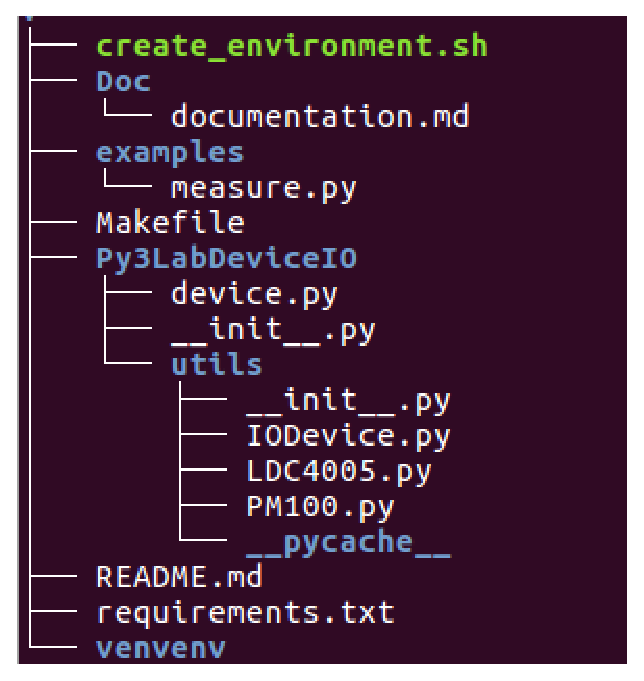
\includegraphics[scale=0.3]{tree.eps}
  \caption{Struktura programu skryptowego.}
  \label{struktura_rys_1}
\end{figure}
\section{Wersja okienkowa programu do pomiarów}
Na rysunku \ref{gui_rys} przedstawiony jest okienkowy program do wykonywania charakterystyk. Program napisany jest w języku
Python 2.7 z wykorzystaniem bibliotek PyQt5, matplotlib
\begin{figure}[h]
\center
  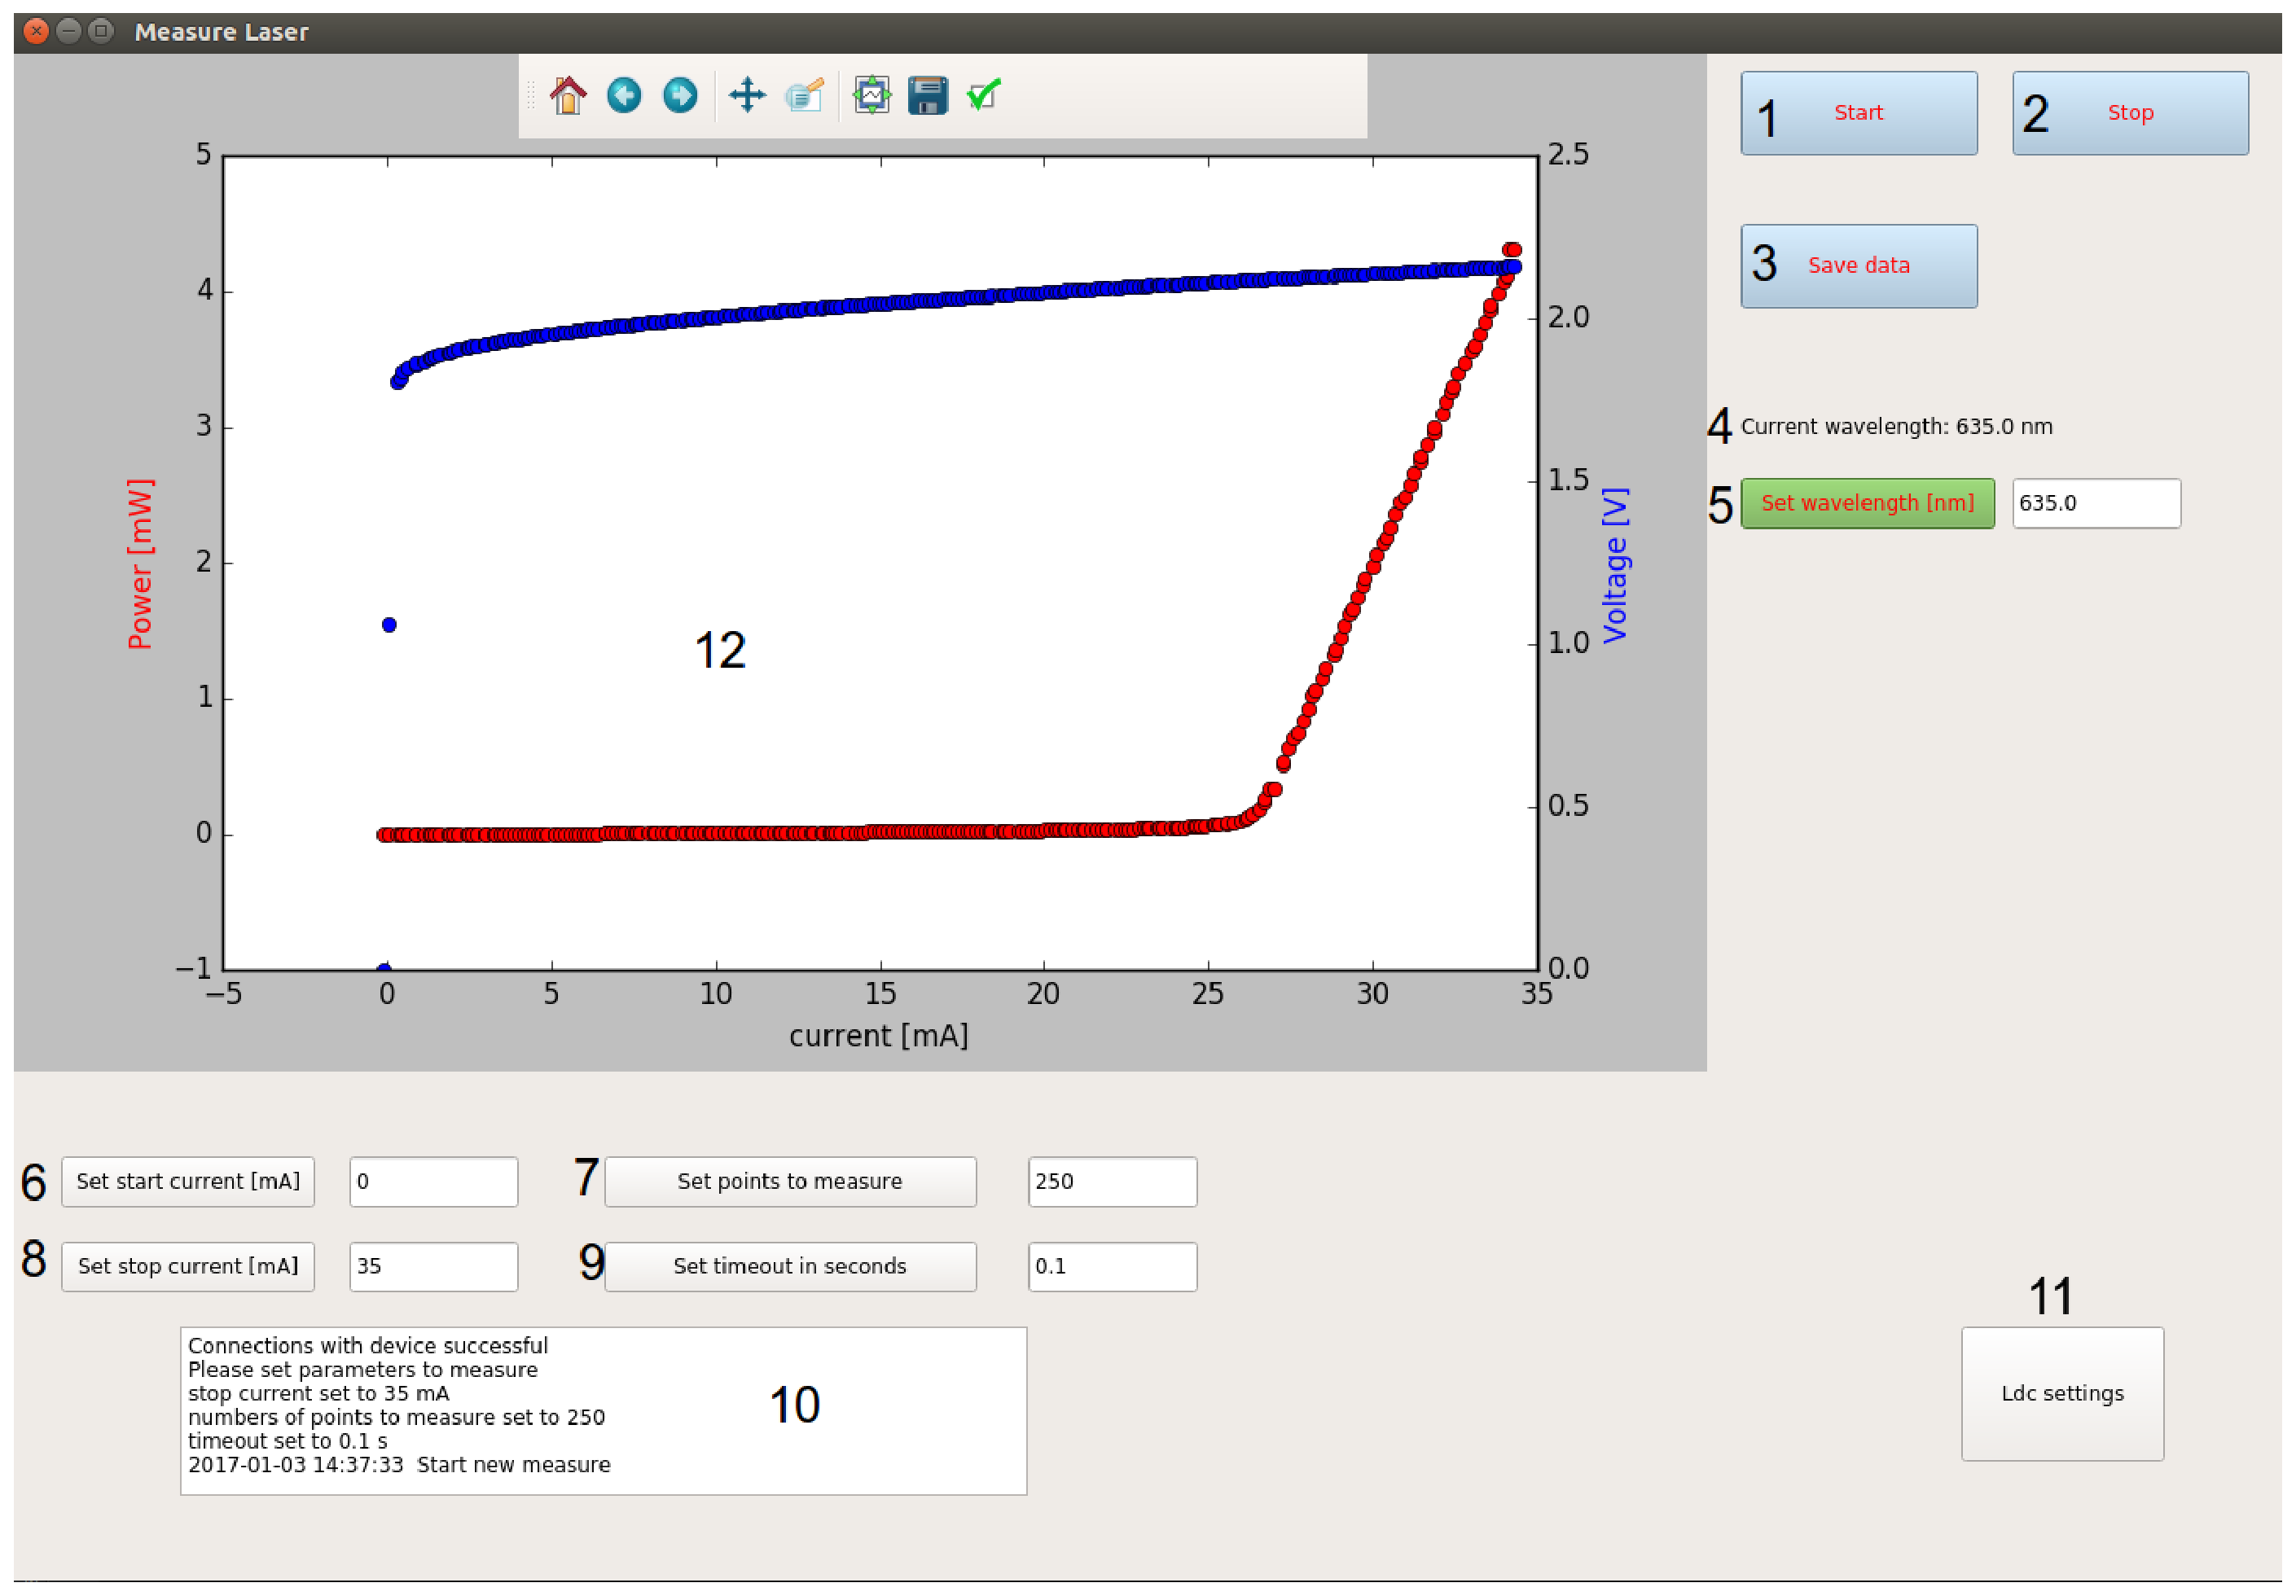
\includegraphics[scale=0.35]{gui.eps}
  \label{gui_rys}
  \caption{1 --- rozpoczecie pomiarów, 2 --- zatrzymanie pomiarów, 3 --- zapisanie danych pomiarowych, 4 --- pokazuje długość fali detektora,
   5 --- zmiana długości fali detektora 6 --- ustawia prąd początkowy do pomiarów, 7 ---  ustawia ilość punktów do pomiaru,
   8 --- ustawia prąd końcowy do pomiarów, 9 --- ustawia długość pauzy pomiędzy pomiarami, 10 --- wyświetla ważne informacje o ustawieniach,
   11 --- ustawienie zasilacza, 12 --- pokazuje charakterystykę.}
\end{figure}
\newpage
\begin{itemize}
\item Przycisk ,,Start" [1] służący do rozpoczęcia pomiarów. Po jego wciśnięciu nastąpi wykonanie charakterystyki lasera na podstawie ustawionych parametrów.
\item Przycisk ,,Stop" [2] służący do zatrzymania pomiarów. Po jego wciśnięciu nastąpi wyłączenie zasilacza.
\item Przycisk ,,Save data" [3] służący do zapisania zebranych danych. Po wciśnięciu należy wybrać ścieżkę. Zapis dokonywany jest w formacie txt.
\item Wyświetlacz długości fali wybranej na detektorze [4]. Długość fali wyświetlana jest w nanometrach.
\item Przycisk służący do zmiany długości fali na detektorze [5]. Wartość należy wprowadzić w nanometrach i zatwierdzić.
\item Przycisk ,,Set start current" [6] --- służy do wybrania prądu, od jakiego ma się zacząć pomiar w mA.
\item Przycisk ,,Set points to measure" [7] --- służy do wybrania ilości punktów do charakterystyki.
\item Przycisk ,,Set stop current" [8] --- służy do wybrania granicy prądu, do jakiego ma się odbyć pomiar w mA.
\item Przycisk ,,Set timeout in seconds" [9] --- służy do ustawienie długości pauzy między zadaniem prądu do zasilacza, a wykonaniem pomiaru.
\item Okienko informacyjne [10] --- wyświetla informacje o pomiarze.
\item Przycisk "Ldc settings" [11] --- ustawia najważniejsze parametry zasilacza diod takie jako wartość maksymalna prądu.
\item Ekran główny [12] --- pokazuje w czasie rzeczywistym zależność napięcia na laserze oraz mocy wyjściowej w funkcji
prądu wejściowego.
\end{itemize}
\newpage
\chapter{Lasery półprzewodnikowe}
\section{Teoria}
\subsection{Teoria pasmowa}
Działanie laserów półprzewodnikowcyh opiera się na prawach, które opisuje teoria pasmowa.
Podstatowe przewidywanie teori pasmowej mówi, że ciało stałe składa się z szeregu pasm rozdzielonych od siebie
 przerwami energetycznymi o skończonych szerokościach wyrażanych w eV. Najważniejszą przerwą, która ma wpływ na właściwości elektryczne ciała jest
 przerwa pomiędzy pasmem walencyjnym, a pasmem przewodnictwa tzw. przerwa energii wzbronione $E_g$. Ze względu na szerokość przerwy
  wyrózniamy ~\cite{laser_book}:
\begin{itemize}
\item izolatory: $E_g > 3$\,eV
\item półprzewodniki: $E_g =$ 0.1\,eV--2.5\,eV
\item przewodniki: $E_g<$0.1\,eV
\end{itemize}
Wartość przewy energetycznej maleje z temperaturą według zależności ~\cite{laser_book}:
\begin{equation}
E_g(T) = E_{g0} - \frac{\alpha T^2}{\beta + T}
\end{equation}
gdzie: $E_{g0}$ --- wartooś przerwy energetycznej w temperaturze $T=0$\,K, \\ $\alpha = 4.5 \cdot 10^{-4}$\,eV/K.
Wartość paramentru $\beta$ jest dodatnia i zależny od rodzaja półprzewodnika, więc im wyższa temperatura tym wartość przerwy mniejsza.
\subsection{Lasery półprzewodnikowe}
Lasery półprzewodnikowe są ważną oraz dynamicznie rozwijączą się gałęzią optoelektroniki. Cały czas są one udoskonalane dzięki
 czemu obejmują corasz szerszy zakres częstości widma oraz potrafią generować promieniowanie o dużych mocach.
 Aby móc udoskonalać  potrzebne są prace zarowno teoretyczne, jak i doświadczarne. Praca ta skupia się na części doświadczarnej.
 Lasery półprzewodnikowe znajduje zastosowanie w telekomunikacji, zapisie informacji.
 Zalety laserów półprzewodnikowych:
 \begin{itemize}
 \item małe wymiary
 \item łatwość modulacji emitowanego promieniowania
 \item niezawodność pracy
 \item proste zasilanie
 \end{itemize}
 \newpage
Lasery półprzewodnikowe inaczej nazywane kwantowe generatory optyczne są laserami złączowymi. Lasery te są źródłem
monochromatycznego oraz skolimowanego promieniowania spójnego. W tego typu laserach ośrodkiem aktywnym jest półprzewodnik.
Obszar czynny zazwyczaj orgraniczony jest do wąskiego paska oraz położony jest w płaszczyźnie złącza p-n.
Pompowanie uzyskiwane jest przez wstrzykiwanie mniejszościowych nośników ładunku do obszaru p-n, które spolaryzowane jest w kierunku przewodzenia.
Rezonator jest zazwyczaj w kształcie prostopadłościanu o wymiarach ułamków milimetra, zazwyczaj wykonany także w materiałe półprzewodnikowym~\cite{publikcja_nakwaski}.
Spreżenie optyczne uzykiwane jest przez zastosowanie pary zwierciadeł prostopadłych do płaszczyzny obszary czynnego lub
za pomocą pofardownaje specjalnie powierzchni która jest równoległa do tego obszaru (DFB - Distributed Feed Back).
Aby zaszła akcja laserowa, prąd zasilający musi przekroczyć pewną wartośc progową zwaną prądem progowym $I_{\mathrm{th}}$, który w dalszej cześci jest
opisywany bardziej szczególowo.
Podstawowym zjawiskiem fizycznym na których swe działanie opierają lasery półprzewodnikowe jest przejście promieniste
czyli proces rekombinacji elektronu i dziury w wyniku którego następuje emisja promieniowania. Gdy prąd osiągnie wystarczająco
dużą wartość dochodzi do inwersji obsadzeń, czyli stanu w którym liczba cząstek o wyszej energi jest większa niż cząsrek o energiach niszych.
Zajście inwersji obsadzeń pozwala wywołać akcję laserową. Emitowana wiążka światła charakteryzuje się niewielką rozbieżnością kątową (kilku stopni). Wśród laserów półprzewodnikowych
wyrozniamy: lasery VCSEL oraz lasery o emisji krawędziowej.
\subsection{Laser VCSEL}
Lasery VCSEL (ang. \textit{Vertical Cavity Surface Emitting Laser}) jest to laser z emisją powierzchniową o pionowej wnęce rezonansowej.
W laserach VCSEL promieniowanie rozchodzi się  w kierunku prostopadłym do krawędzi obszaru czynnego oraz wzmacniane jest jedynie
wewnątrz tego obszaru ~\cite{publikcja_nakwaski}.
\subsection{Laser o emisji krawędziowej}
Laser krawędziowy są to laser z wnęka w  płaszczyźnie warstwy aktywnej. Charakteryzują się większą wartością prądu prowego
oraz większą sprawnością niż laser VCSEL. Te cechy laserów są tematem moich badań.
\subsection{Prąd progowy}
Charakterystyka wyjściowa lasera przedstawia zależność napięcia na laserze oraz mocy wyjściowej w funckji aplikowanego prądu.
Ważnym parametrem laserów półprzewodnikowych jest prąd progowy (z ang. \textit{threshold
current}) który określa wartość prądu, przy którym zaczyna zachodzić akcja laserowa, czyli
rośnie gwałtownie natężenie promieniowania i maleje szerokość linii emisyjnej. W celu wyznaczenia prądu progowego należy
sporządzić wykres zależności mocy wyjściowej lasera od prądu zasilającego. Następnie dla prądu gdzie zaczyna się akcja
laserowa dla odcinka liniowego należy metodą najmniejszych kwadratów przy użyciu wielomianu pierwszego stopnia(\ref{eq:fit_i_th})
 znaleźć parametry prostej o parametrach $a$ i $b$.
 Dla wyznaczonej krzywej należy znaleźć miejsce zerowe, które będzie wyznaczonym prądem progowym $I_{\mathrm{th}}$(\ref{eg:i_th}).
\begin{equation}
\label{eq:fit_i_th}
P = a \cdot I + b
\end{equation}
\begin{equation}
\label{eg:i_th}
I_{\mathrm{th}} = -\frac{b}{a}
\end{equation}
\begin{equation}
\Delta I_{\mathrm{th}} = \left\lvert \frac{\partial I_{th}}{\partial a} \right\rvert \cdot \Delta a + \left\lvert \frac{\partial I_{th}}{\partial b} \right\rvert \cdot \Delta b
\end{equation}
\begin{equation}
\Delta I_{\mathrm{th}} = \left\lvert -\frac{b}{a^2} \right\rvert \cdot \Delta a + \left\lvert -\frac{1}{a} \right\rvert \cdot \Delta b
\end{equation}
Dla laserów krawędziowych prąd progowy rośnie wraz z temperaturą, co może być scharakteryzowane za pomocą parametru
$T_{0}$ wyrażonego w kelwinach tzw. temperatury charakterystycznej~\cite{opto_book}.
Dla laserów krawędziowych zależności prądu progowego $I_{th}$ od temperatury $T$ wyrażamy w postaci równania:
\begin{equation}
\label{eq:i_th}
I_{\mathrm{th}} = I_0 \exp \left( \frac{T}{T_0} \right)
\end{equation}
Przez zlogarytmowanie wartości prądu oraz podstawienie otrzymujemy:
\begin{equation}
\ln(I_{\mathrm{th}}) =    \frac{T}{T_0}  + \ln(I_0)
\end{equation}
Wartości parametrów $I_0$ oraz $T_0$ możemy wyznaczyć na podstawie charakterystyk
emisyjnych lasera w różnych temperaturach $T$. \\
Mając wartości prądu progowego w danej temperaturze  można do nich dopasować funkcje liniową w postaci:
\begin{equation}
y = a \cdot T + b
\end{equation}
Gdzie:
\begin{equation}
y = \ln(I_{\mathrm{th}})
\end{equation}
\begin{equation}
a = \frac{1}{T_0}
\end{equation}
\begin{equation}
b = \ln(I_0)
\end{equation}
Na tej podstawie możemy znaleźć poszukiwane parametry $I_0$ oraz $T_0$:
\begin{equation}
I_0 = \mathrm{e}^b
\end{equation}
\begin{equation}
T_0 = \frac{1}{a}
\end{equation}
Korzystając z metody różniczki zupełnej można obliczyć wartości błędów wyznaczonych wartości:
\begin{equation}
\Delta I_0 = \left\lvert \frac{\partial I_{0}}{\partial b} \right\rvert \cdot \Delta b = | \mathrm{e}^b | \cdot \Delta b
\end{equation}
\begin{equation}
\Delta T_0 = \left\lvert \frac{\partial T_{0}}{\partial a} \right\rvert \cdot \Delta a = \left\lvert -\frac{1}{a^2} \right\rvert \cdot \Delta a
\end{equation}
Dla laserów VCSEL nie można zastować powyszej zależności (\ref{eq:fit_i_th}).
\subsection{Sprawność}
Innym ważnym parametrem, którym możemy scharakteryzować lasery półprzewodnikowe jest ich sprawność. Można wyróżnić następujące rodzaje sprawności:
\begin{itemize}
\item Sprawność różniczkowa (ang. \textit{slope efficiency}) --- jest zdefiniowana jako nachylenie krzywej uzyskanej przez wykreślenie zależności
mocy wyjściowej z lasera versus energii dostarczonej do lasera w postaci natężenie prądu $I$ lub moc dostarczonej $P$. Sposób wyznaczanie sprawności
przedstawiony jest na rysunku~\ref{fig:teoria_rys_2}
Moc dostarczoną definujemy jako:
\begin{equation}
P = U \cdot I
\end{equation}
gdzie: $U$ --- napięcie na laserze.
\item Sprawność całkowita (ang. \textit{wall-plug-efficiency}) --- jest zdefiniowana jako stosunek mocy wyjściowej do całkowitej mocy wejściowej lasera.
\end{itemize}
\subsection{Funkcja Fermiego}
Na sprawność laserów półprzewodnikowych duży wpływ ma funkcja rozkładu Fermiego-Diraca przedstawiony na rysunku~\ref{fig:teoria_rys_3},
. Funkcja Fermiego-Diraca opisuje prawdopodobieństwo obsadzenia przez elektron poziomu
energetynczego $E$ przy temperaturze $T$
\begin{equation}
f(E) = \frac{1}{e^{(E-E_F)/kT} + 1}
\end{equation}
gdzie: $E_f$ --- energia fermiego. \\
Wraz z wzrostem temperatury rośnie prawdopodobieństwo obszadzenia wyższego stanu energetynczego przez elektron. Ma to
wpływ na sprawność różniczkową lasera półprzewodnikowego. Wraz z wzrostem temperatury spraność maleje, spowodowane jest to ostrzeniem
widma wzmocnienia, gdy rozkład fermiego się zweżą(narrowing)~\cite{publikacja_1}.
%Poziom fermiego reprezentuje średnią pracę którą należy wykonać aby usunąć elektron z materiału.
\begin{figure}[H]
\center
  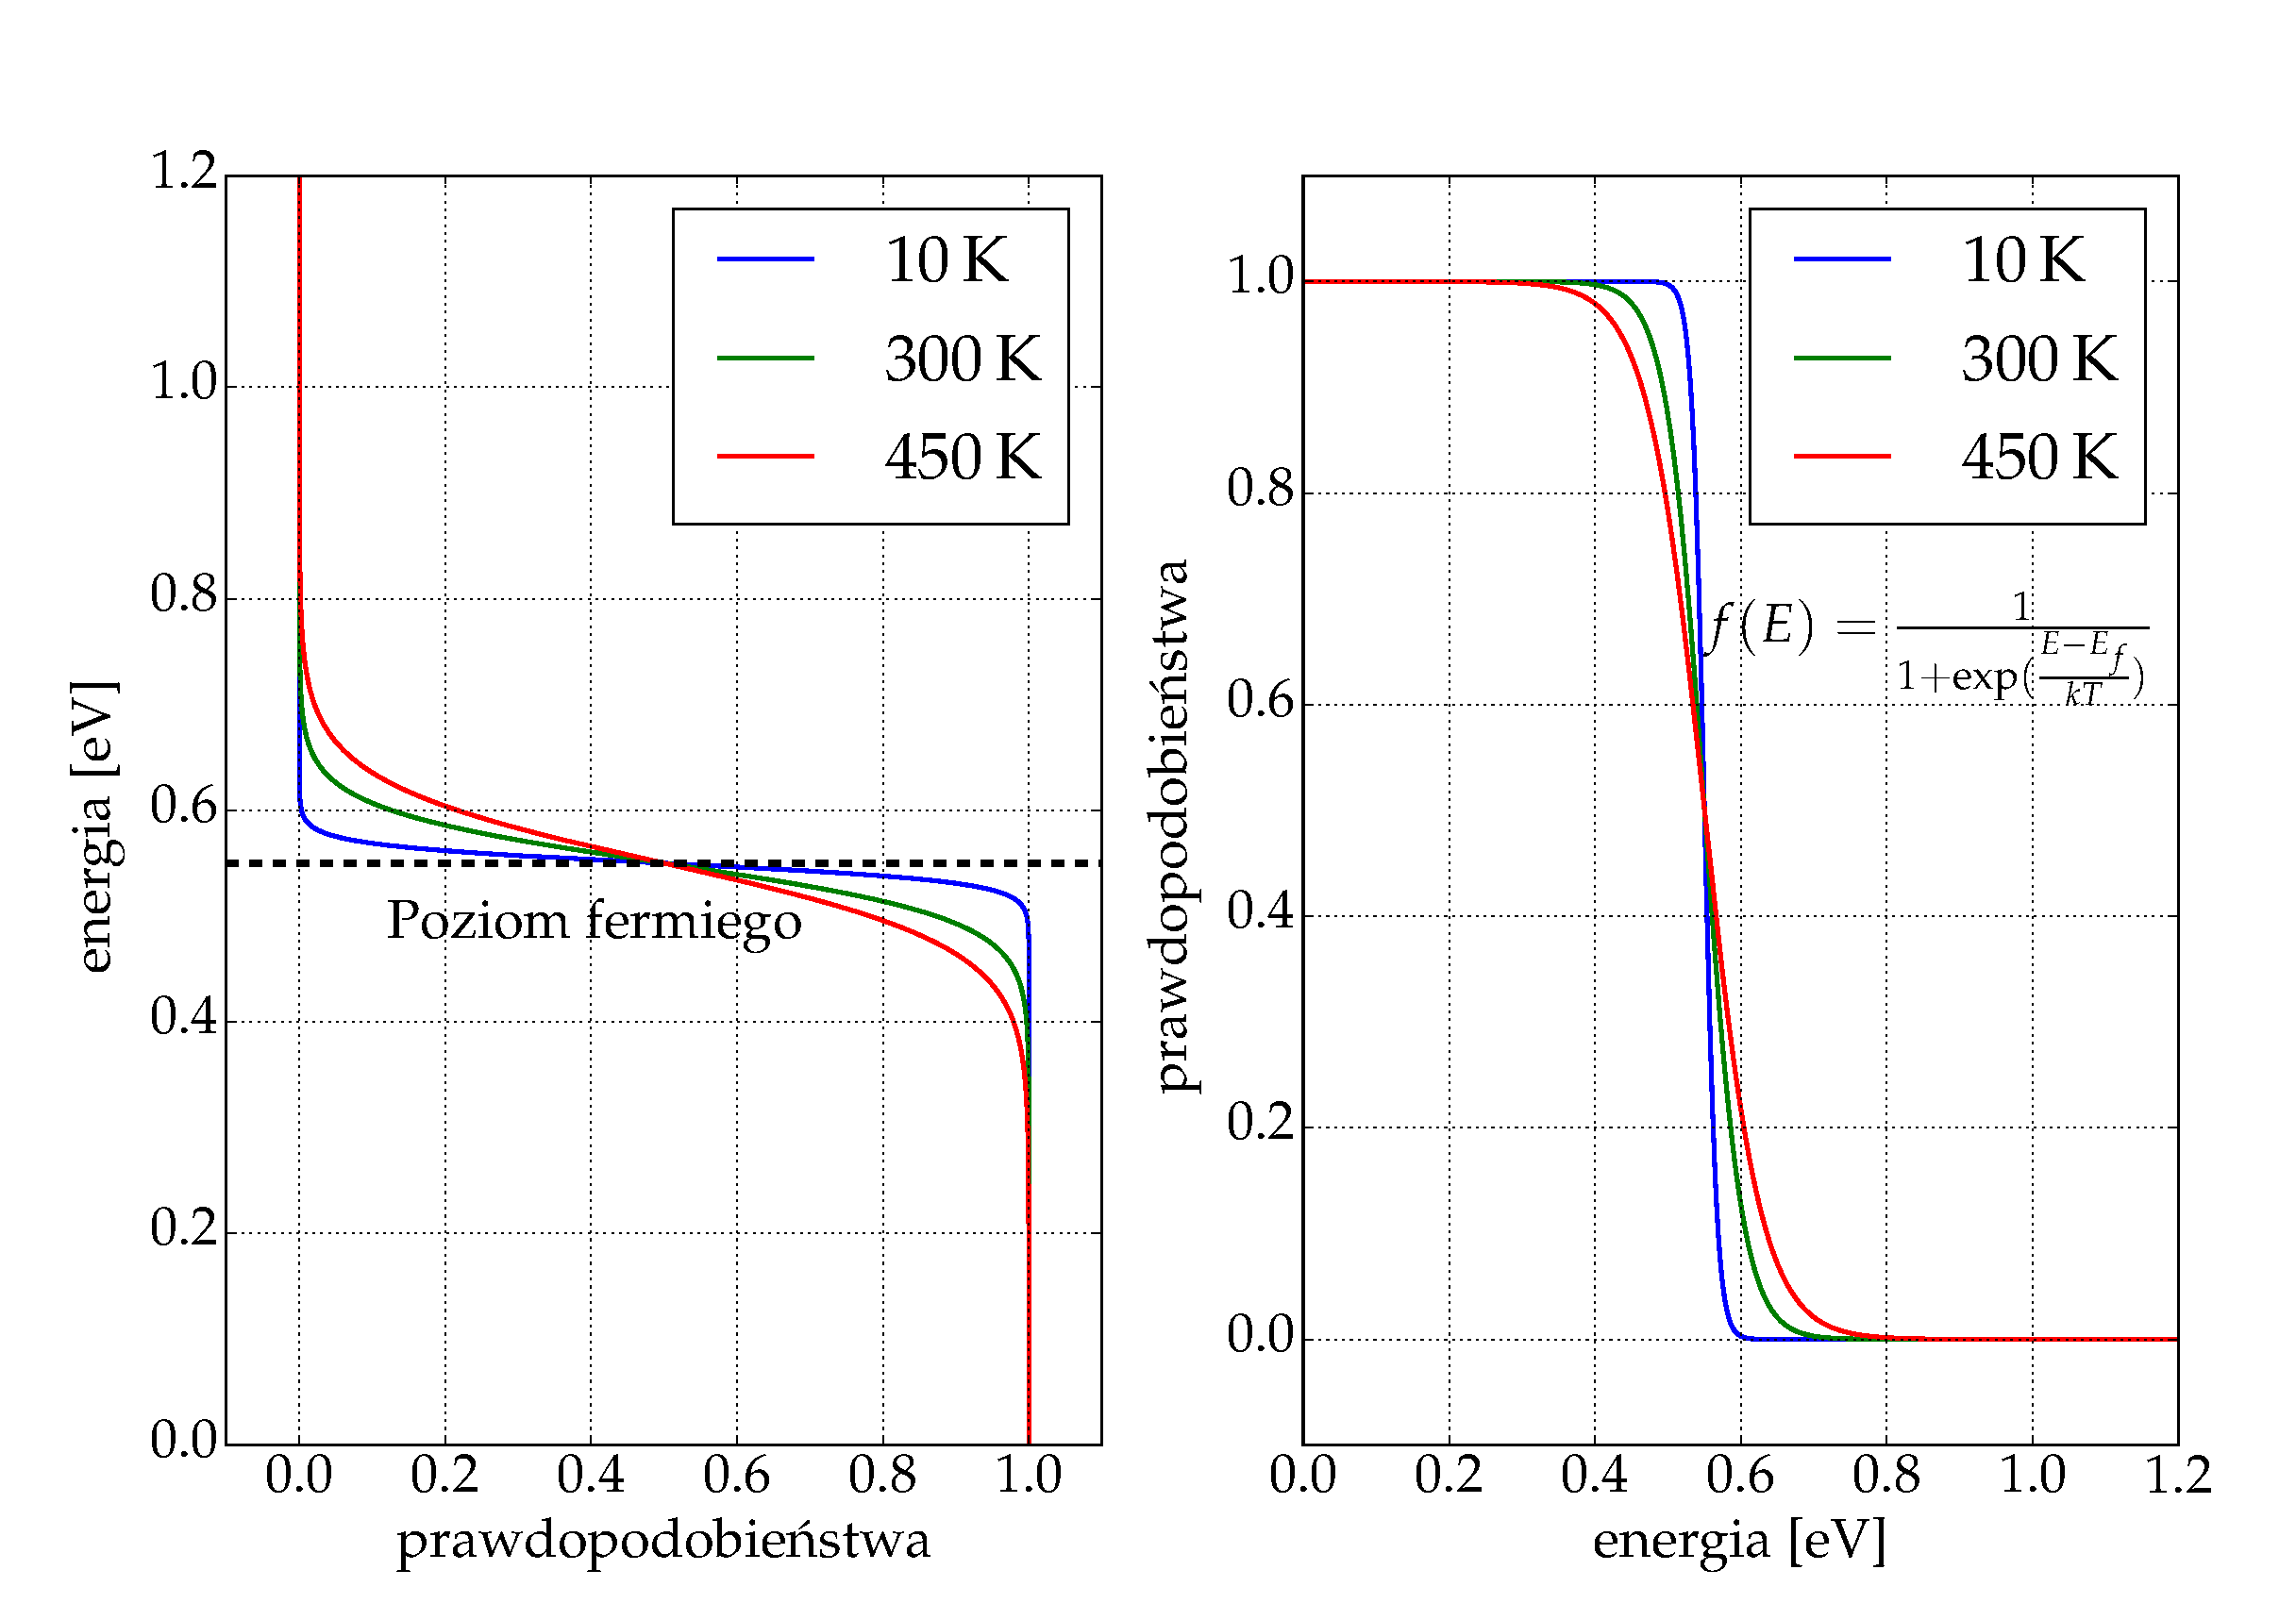
\includegraphics[scale=0.30]{fermi.eps}
  \caption{Rozkład fermiego dla różnych temperatur $T$.}
  \label{fig:teoria_rys_3}
\end{figure}
\newpage
\subsection{Wpływ temperatury chłodnicy lasera na jego paramentry}
Wraz ze wzrostem temperatury wartość prądu progowego $I_{\mathrm{th}}$ rośnie, natomiast sprawność różniczkowa $\eta$ maleje. Jest to spowodowane przez:
\begin{itemize}
\item W wyższych temperaturach funkcja Fermiego-Diraca, która opisuje prawdopodobieństwo zajmowania stanów energetycznych staje się bardziej "rozmarzana".
 Przez co obrządzenie poziomów energetycznych jest bliższe powłoce przewodzenia dla elektronów oraz bliższe powłoce walencyjnej dla dziur.
  Dzięki temu możliwość wzmocnienia promieniowania lasera na długości fali emitowanej jest zredukowane.
\item Dodatkowo w podwójnym aktywnym regionie heterostruktury, rozkład energii elektronów i dziur w wyższych temperaturach jest przesunięty dalej od krawędzi pasma, przez co zwiększa się prawdopodobieństwo pobytu ładunków w aktywnym regionie, co powoduje obniżenie sprawności $\eta$
\item Wraz ze wzrostem temperatury rośnie współczynnik Auger, obniżając wydajność i czas życia ładunku podczas przejścia promienistego, co zwiększa wartość prądu progowego $I_{\mathrm{th}}$.
\end{itemize}
%Sprawność różniczkowa zarówno dla laserów VCSEL i krawędziowych zwiększa się wraz z spadkiem temperatury chłodnicy lasera.
%Jest to spodowane wyostrzaniem(ang. sharpening) się widma wzmocnienia na skutek zwężania się funkcji rozkładu Fermiego.

\newpage
\chapter{Opis eksperymentu}
\section{Układ pomiarowy}
Układ pomiarowt składał się z:
\begin{itemize}
\item Komputera z systemem Linux (Ubuntu) --- wymagane jest, aby na komputerze zainstalowany był język Python wraz z bibliotekami:
matplotlib, numpy, PyQt5. Do sterowania sprzętem przy pomocy programów opisanych w 3 rozdziale wymagane są uprawnienia administratora.
\item Zasilacza diod laserowych firmy Thorlabs model LDC4005~\cite{Ldc_book}--- zapewnia stabilne zasilanie prądowe lasera prądem do 5\,A.
Możliwe jest zasilanie ciągłe i impulsowe. Posiada interfejsem SCPI~\cite{Ldc_book_prog}, umożliwiający sterowanie za pomocą komputera przez USB.
\item Miernik mocy firmy Thorlas firmy Thorlabs model PM100~\cite{Pm100_book} --- stworzony do mierzenia mocy wyjściowej z lasera. Pozwala operować na
długościach fali od 400\,nm do 1100\,nm. Posiada interfejsem SCPI~\cite{Pm100_book}, umożliwiający sterowanie za pomocą komputera przez USB.
\item Kontroler temperatury diod laserowych firmy Thorlabs--- precyzyjny kontroler temperatury pozwalający na zmiany temperatury
chłodniczy lasera podczas operowania prądami do 2\,A.
\end{itemize}
\subsection{Przebieg pomiarów}
Laser był umieszczony w mocowaniu stabilizującym temperaturę diod laserowych połączony z zasilaczem diod laserowych oraz kontrolerem temperatury.
Na wyjściu lasera umieszczony był miernik mocy. Komunikacja z zasilaczem oraz miernikiem odbywała się za pomocą standardu
komend SCPI przez połączenie USB przez wykorzystanie programów opisanych w rozdziale 3.
Temperatura była zmieniana manualnie na kontrolerze temperatury.
Charakterystyki wyjściowe (czyli wartości prądu zasilania, napięcia na laserze oraz mocy wyjściowej)
mierzone były przy pomocy zasilania ciągłego. Wyniki zapisywane były w pliku tekstowym. Schematyczny rysunek układu pomiarowego przedstawiony jest
na rysunku 5.1.
\begin{figure}
\center
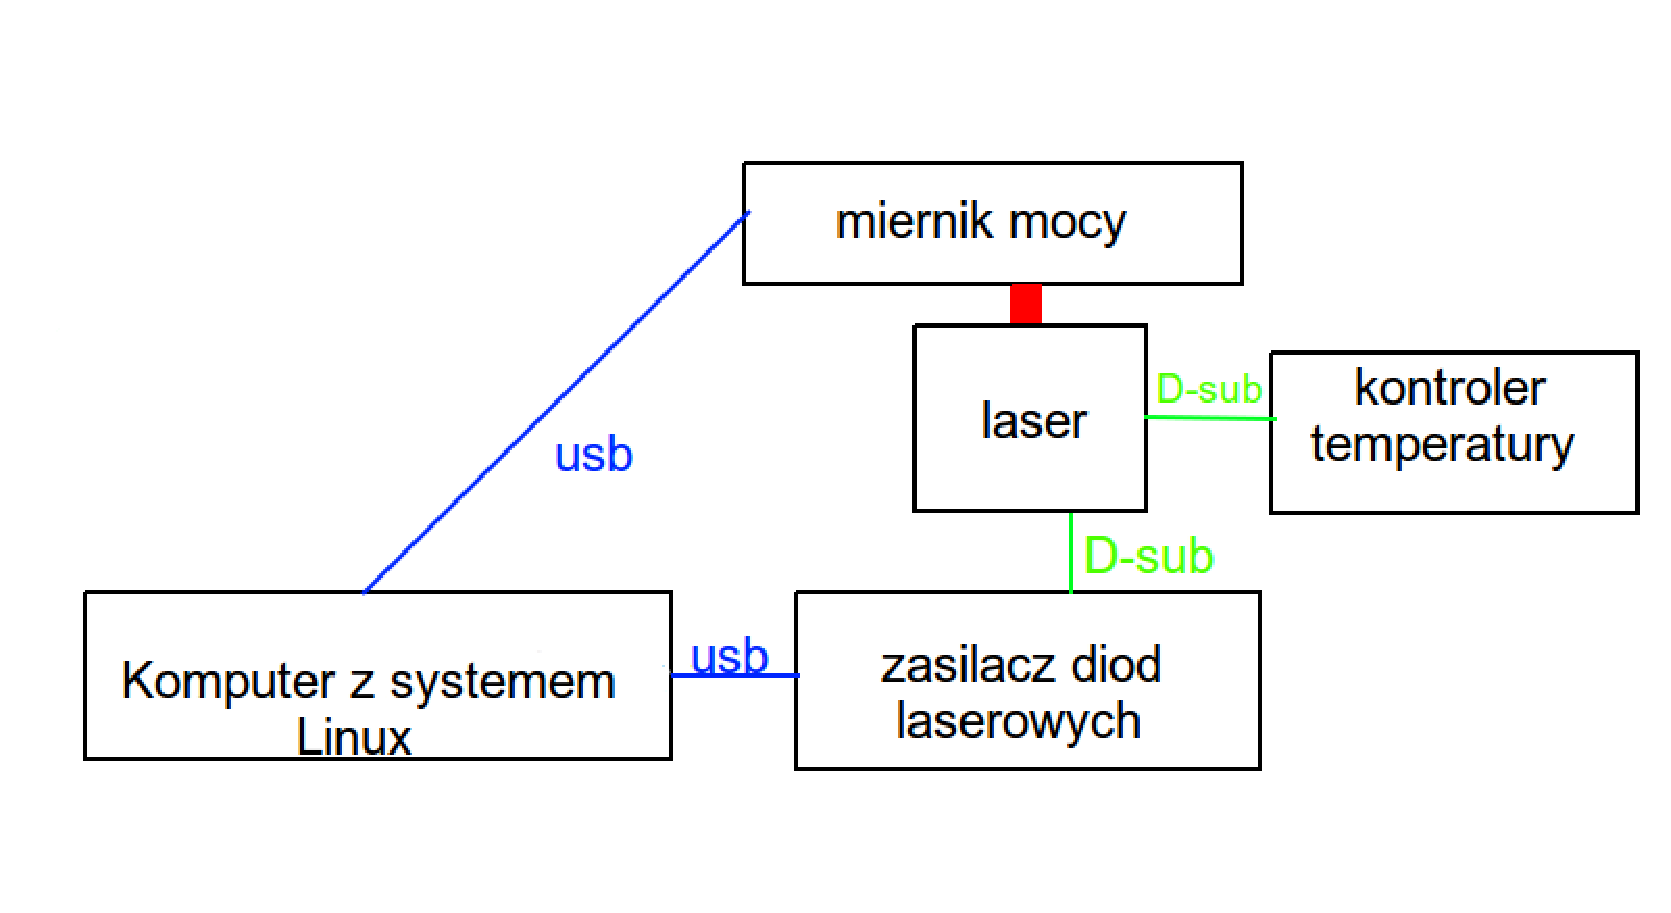
\includegraphics[scale=0.35]{schemat.eps}
\label{fig:sch_pom}
\caption{Schemat układu pomiarowego.}
\end{figure}
\newpage
\section{Laser 635\,nm}
\begin{table}
\begin{center}
\caption{ Wyznaczone wartośc prądu progowego $I_{\mathrm{th}}$ w różnych temperaturach $T$ dla lasera krawędziowego 635\,nm. }
\begin{tabular}{ | C{1.5cm}|  C{1.5cm} | C{1.5cm} | C{1.5cm}| C{1.5cm} | C{1.5cm}| C{1.5cm}| C{2.0cm}| C{2.0cm}|}
\hline
$T$ [K] 	&   278 & 283  	& 288 & 293 & 298 & 303 & 308 \\ \hline
$I_{\mathrm{th}}$ [mA]  &	19.1 $\pm$ 0.2  & 20.7 $\pm$ 0.2 & 22.6 $\pm$ 0.2 &
25.0 $\pm$ 0.2  & 27.9 $\pm$ 0.3 & 31.4 $\pm$ 0.5 & 36 $\pm$ 2	\\ \hline
\end{tabular}
\end{center}
\end{table}
%\begin{figure}
%\center
%  \includegraphics[scale=0.30]{plot635/plot_ivl_4.eps}
%  \label{rys1}
%  \caption{Wykres napięcia i mocy od prądu dla lasera krawędziowego 635\,nm.}
%\end{figure}
\begin{figure}
\center
  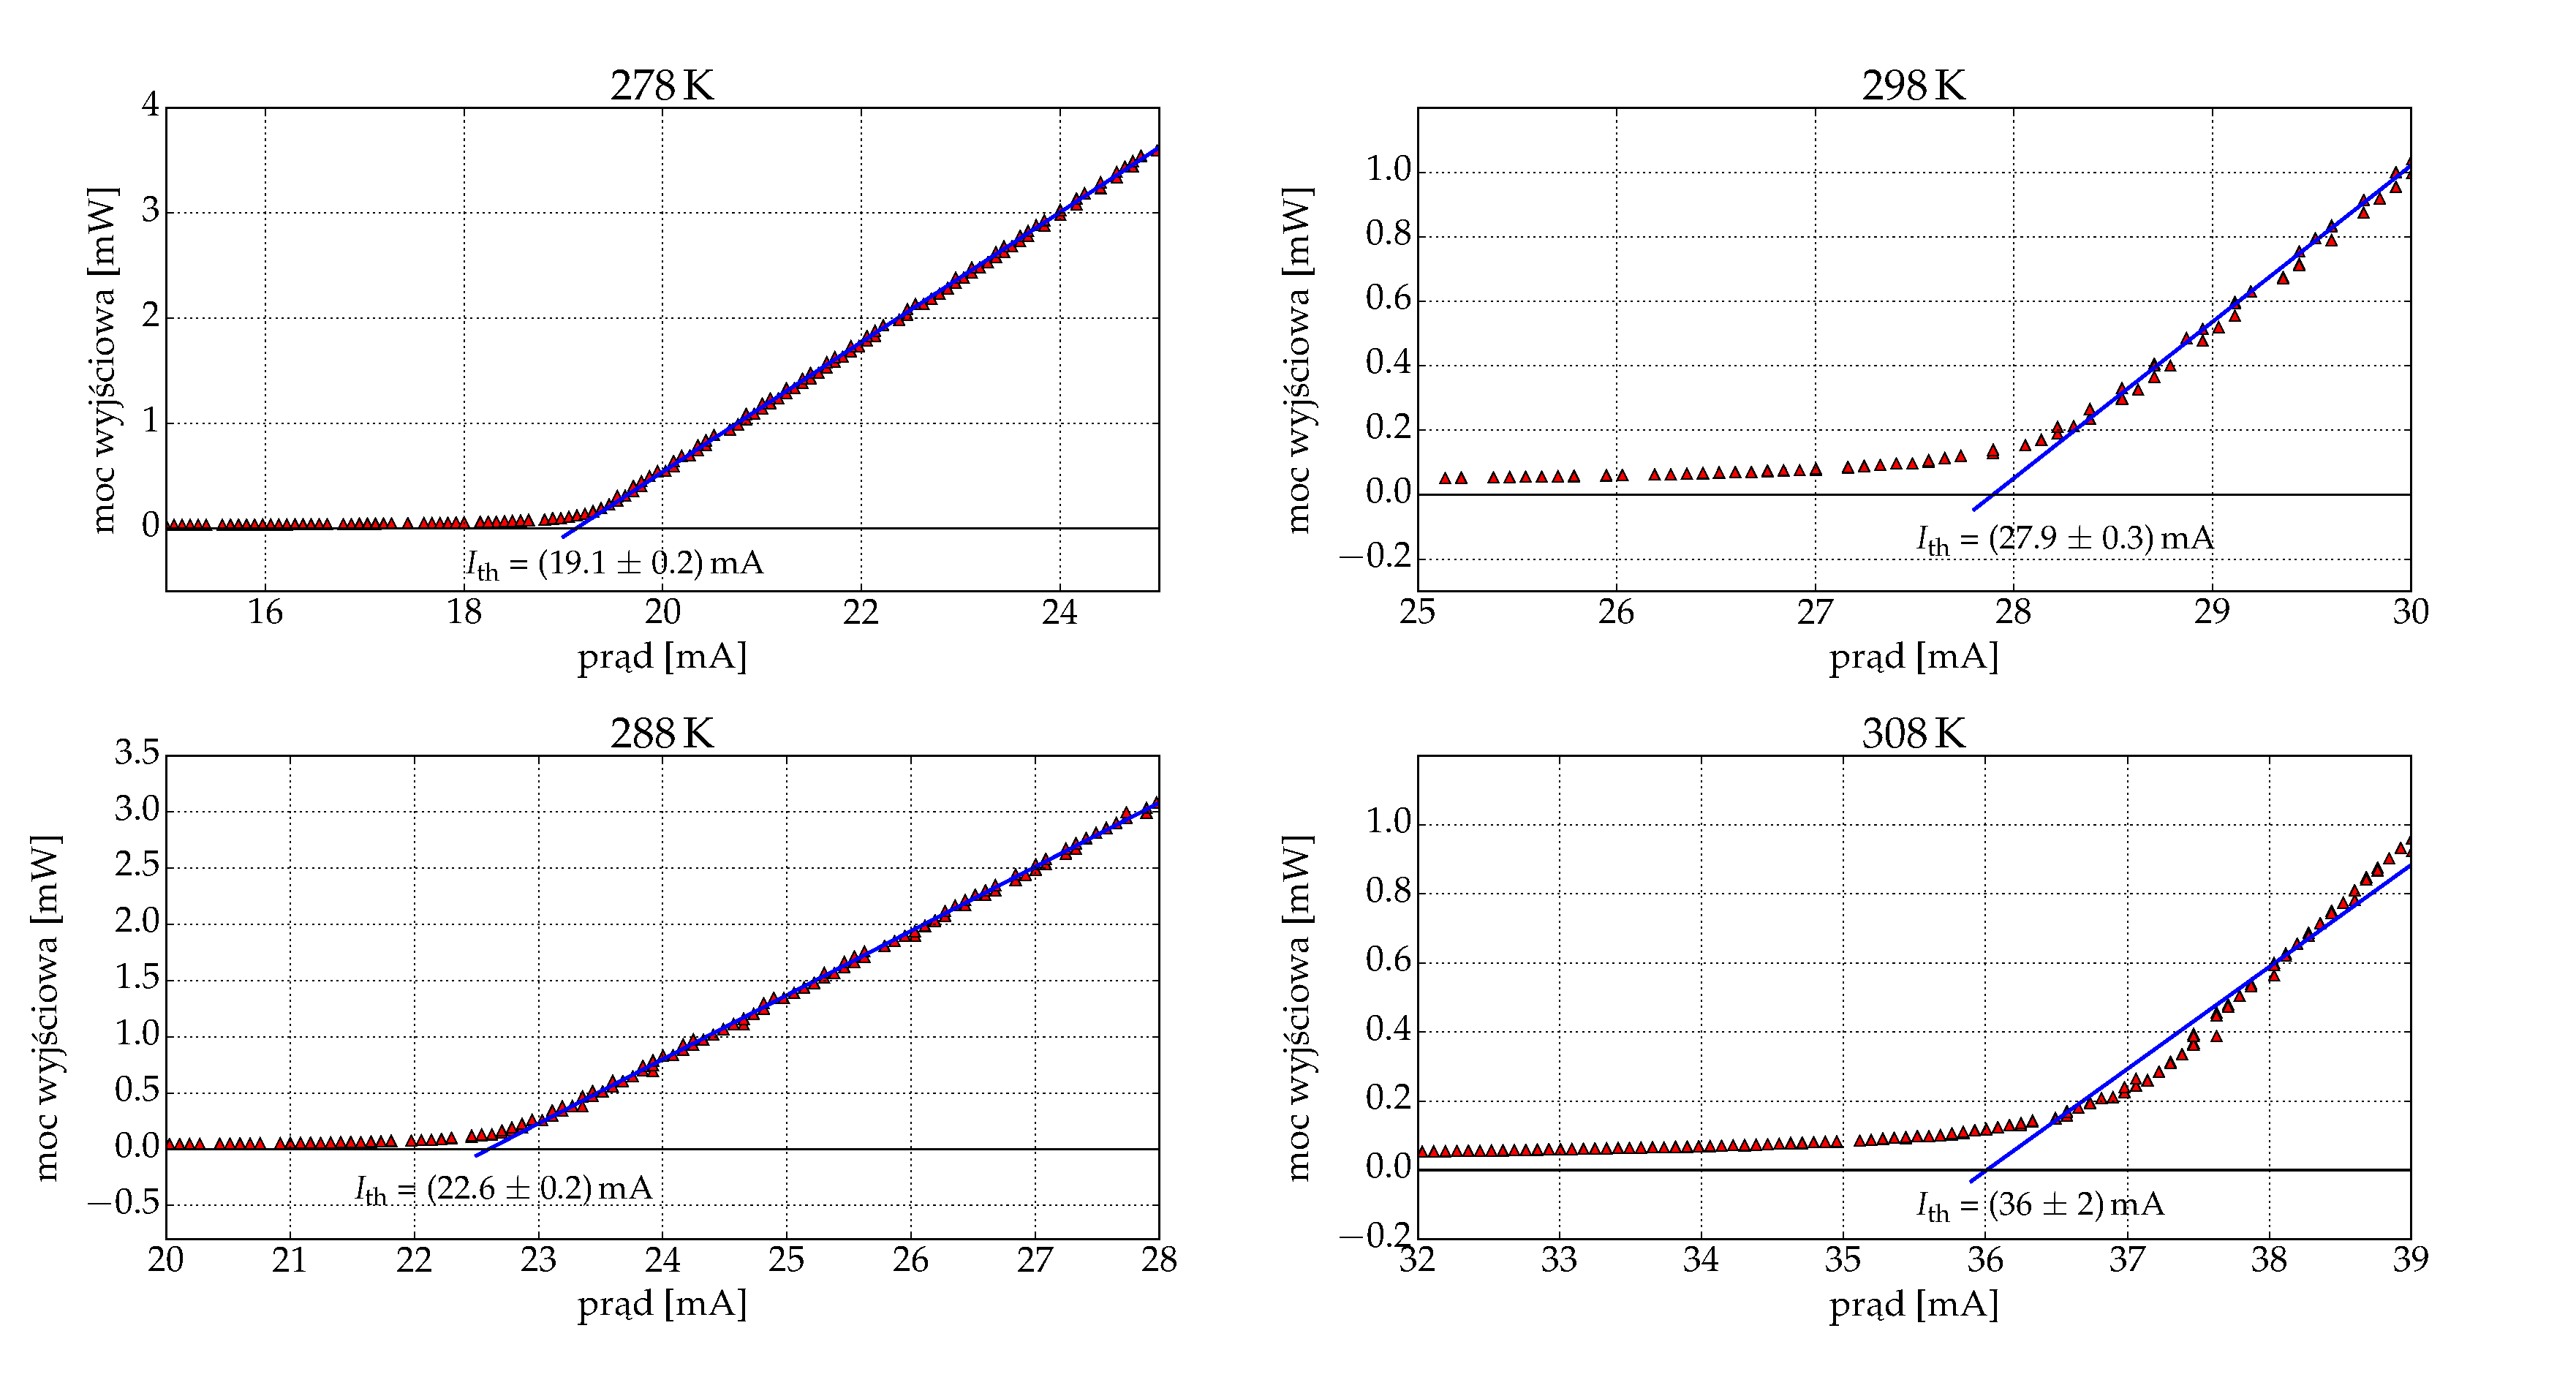
\includegraphics[scale=0.30]{plot635/plot_i_th_4.eps}
  \label{rys2}
  \caption{Wykres prądu progowego dla lasera krawędziowego 635\,nm.}
\end{figure}
\begin{figure}
\center
  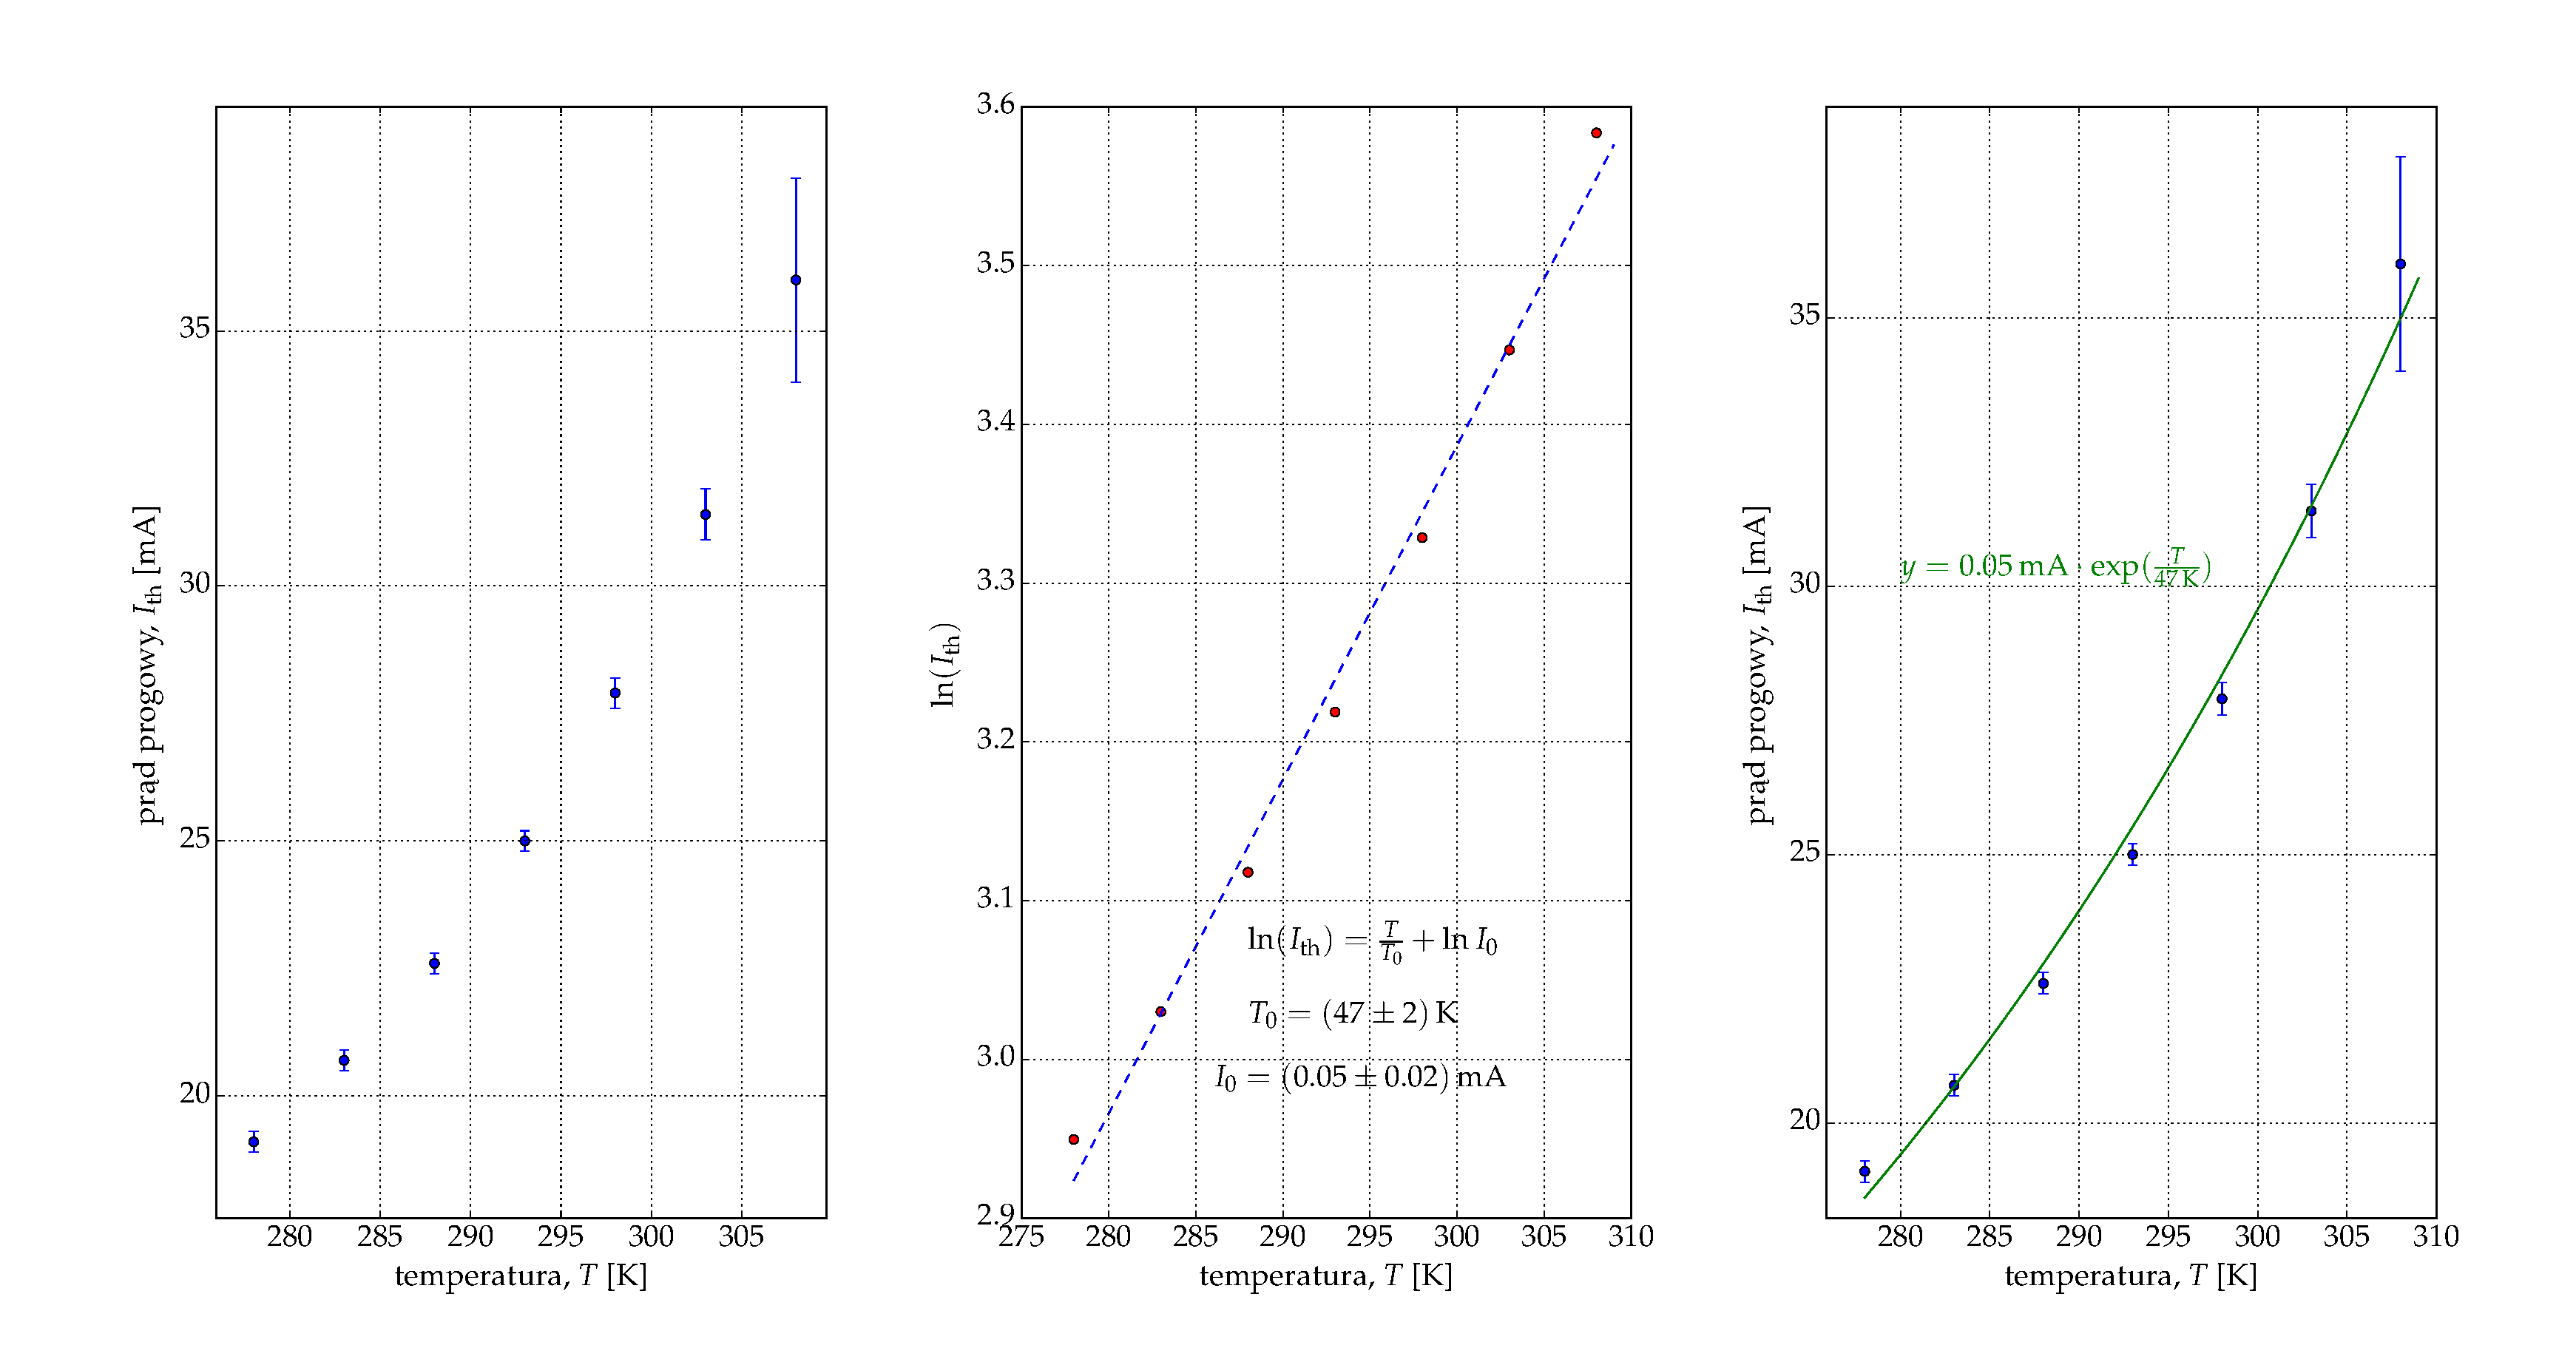
\includegraphics[scale=0.30]{plot635/plot_fit.eps}
  \label{rys2}
  \caption{Wykres prądu progowego z dopasowanymi wartościami $I_{0}$ i $T_{0}$ dla lasera krawędziowego 635\,nm.}
\end{figure}
\begin{figure}
\center
  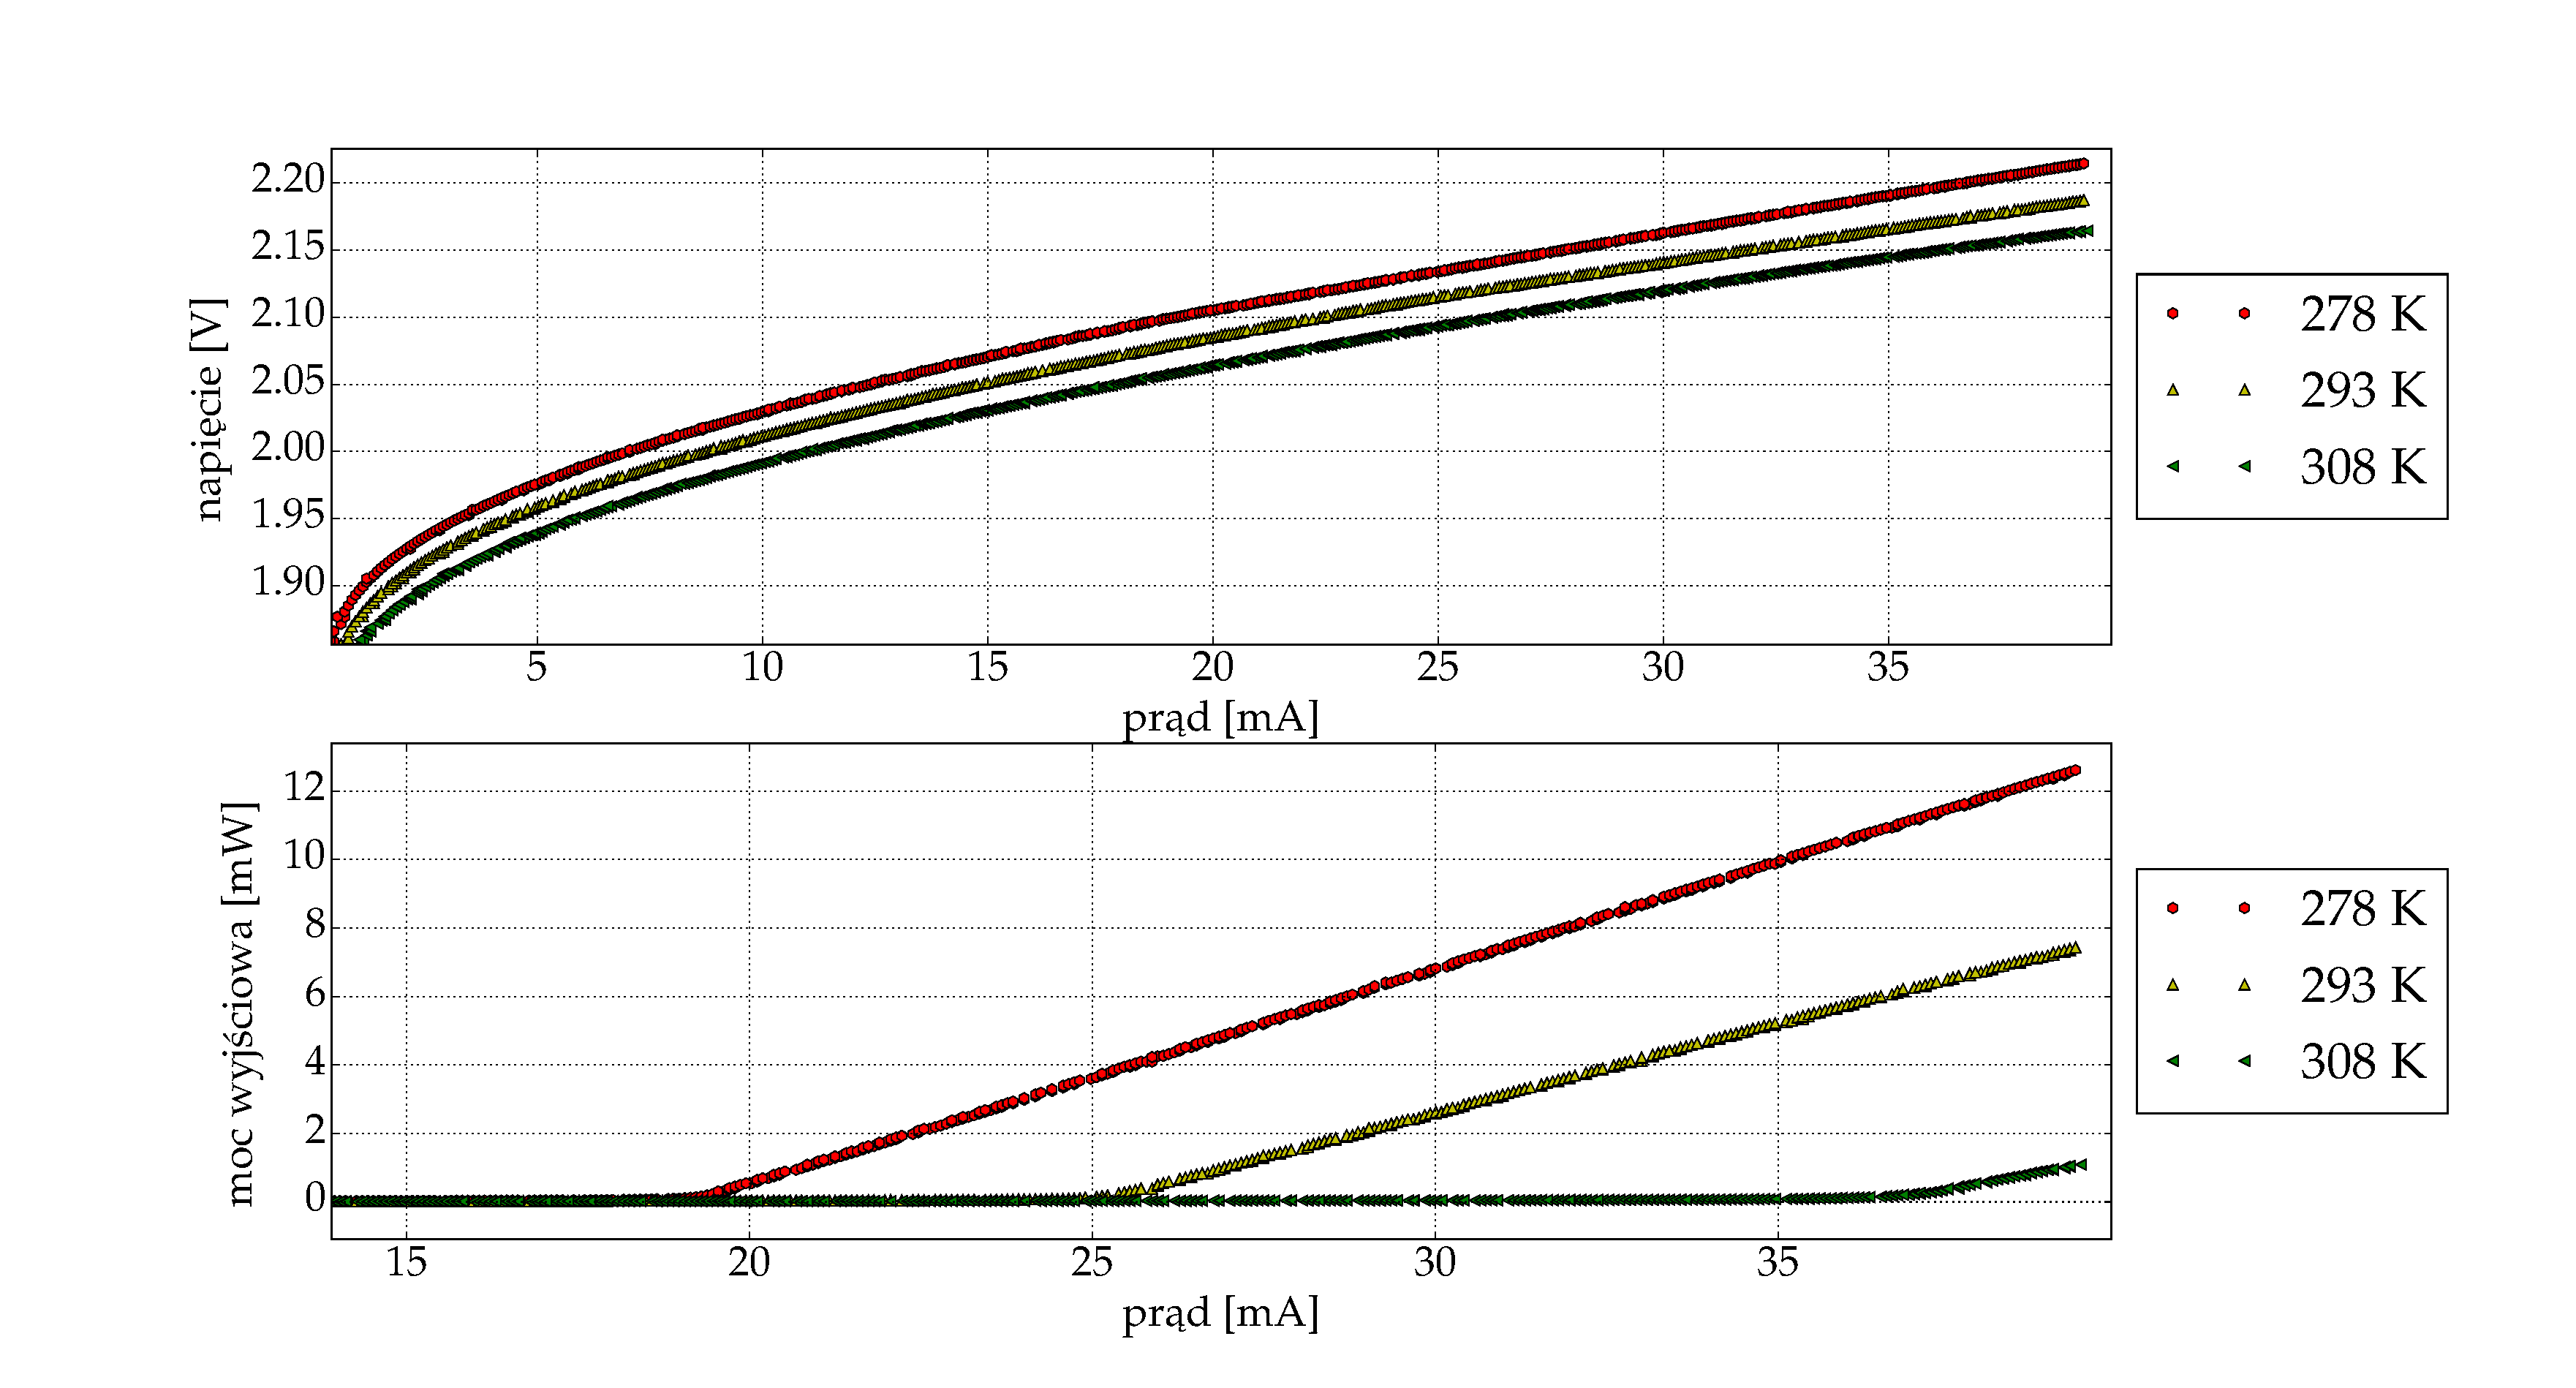
\includegraphics[scale=0.30]{plot635/plot_voltage_power.eps}
  \label{rys3}
  \caption{Wykres napięcia na laserze oraz mocy w funkcji prądu dla lasera krawędziowego 635\,nm.}
\end{figure}
\begin{figure}
\center
  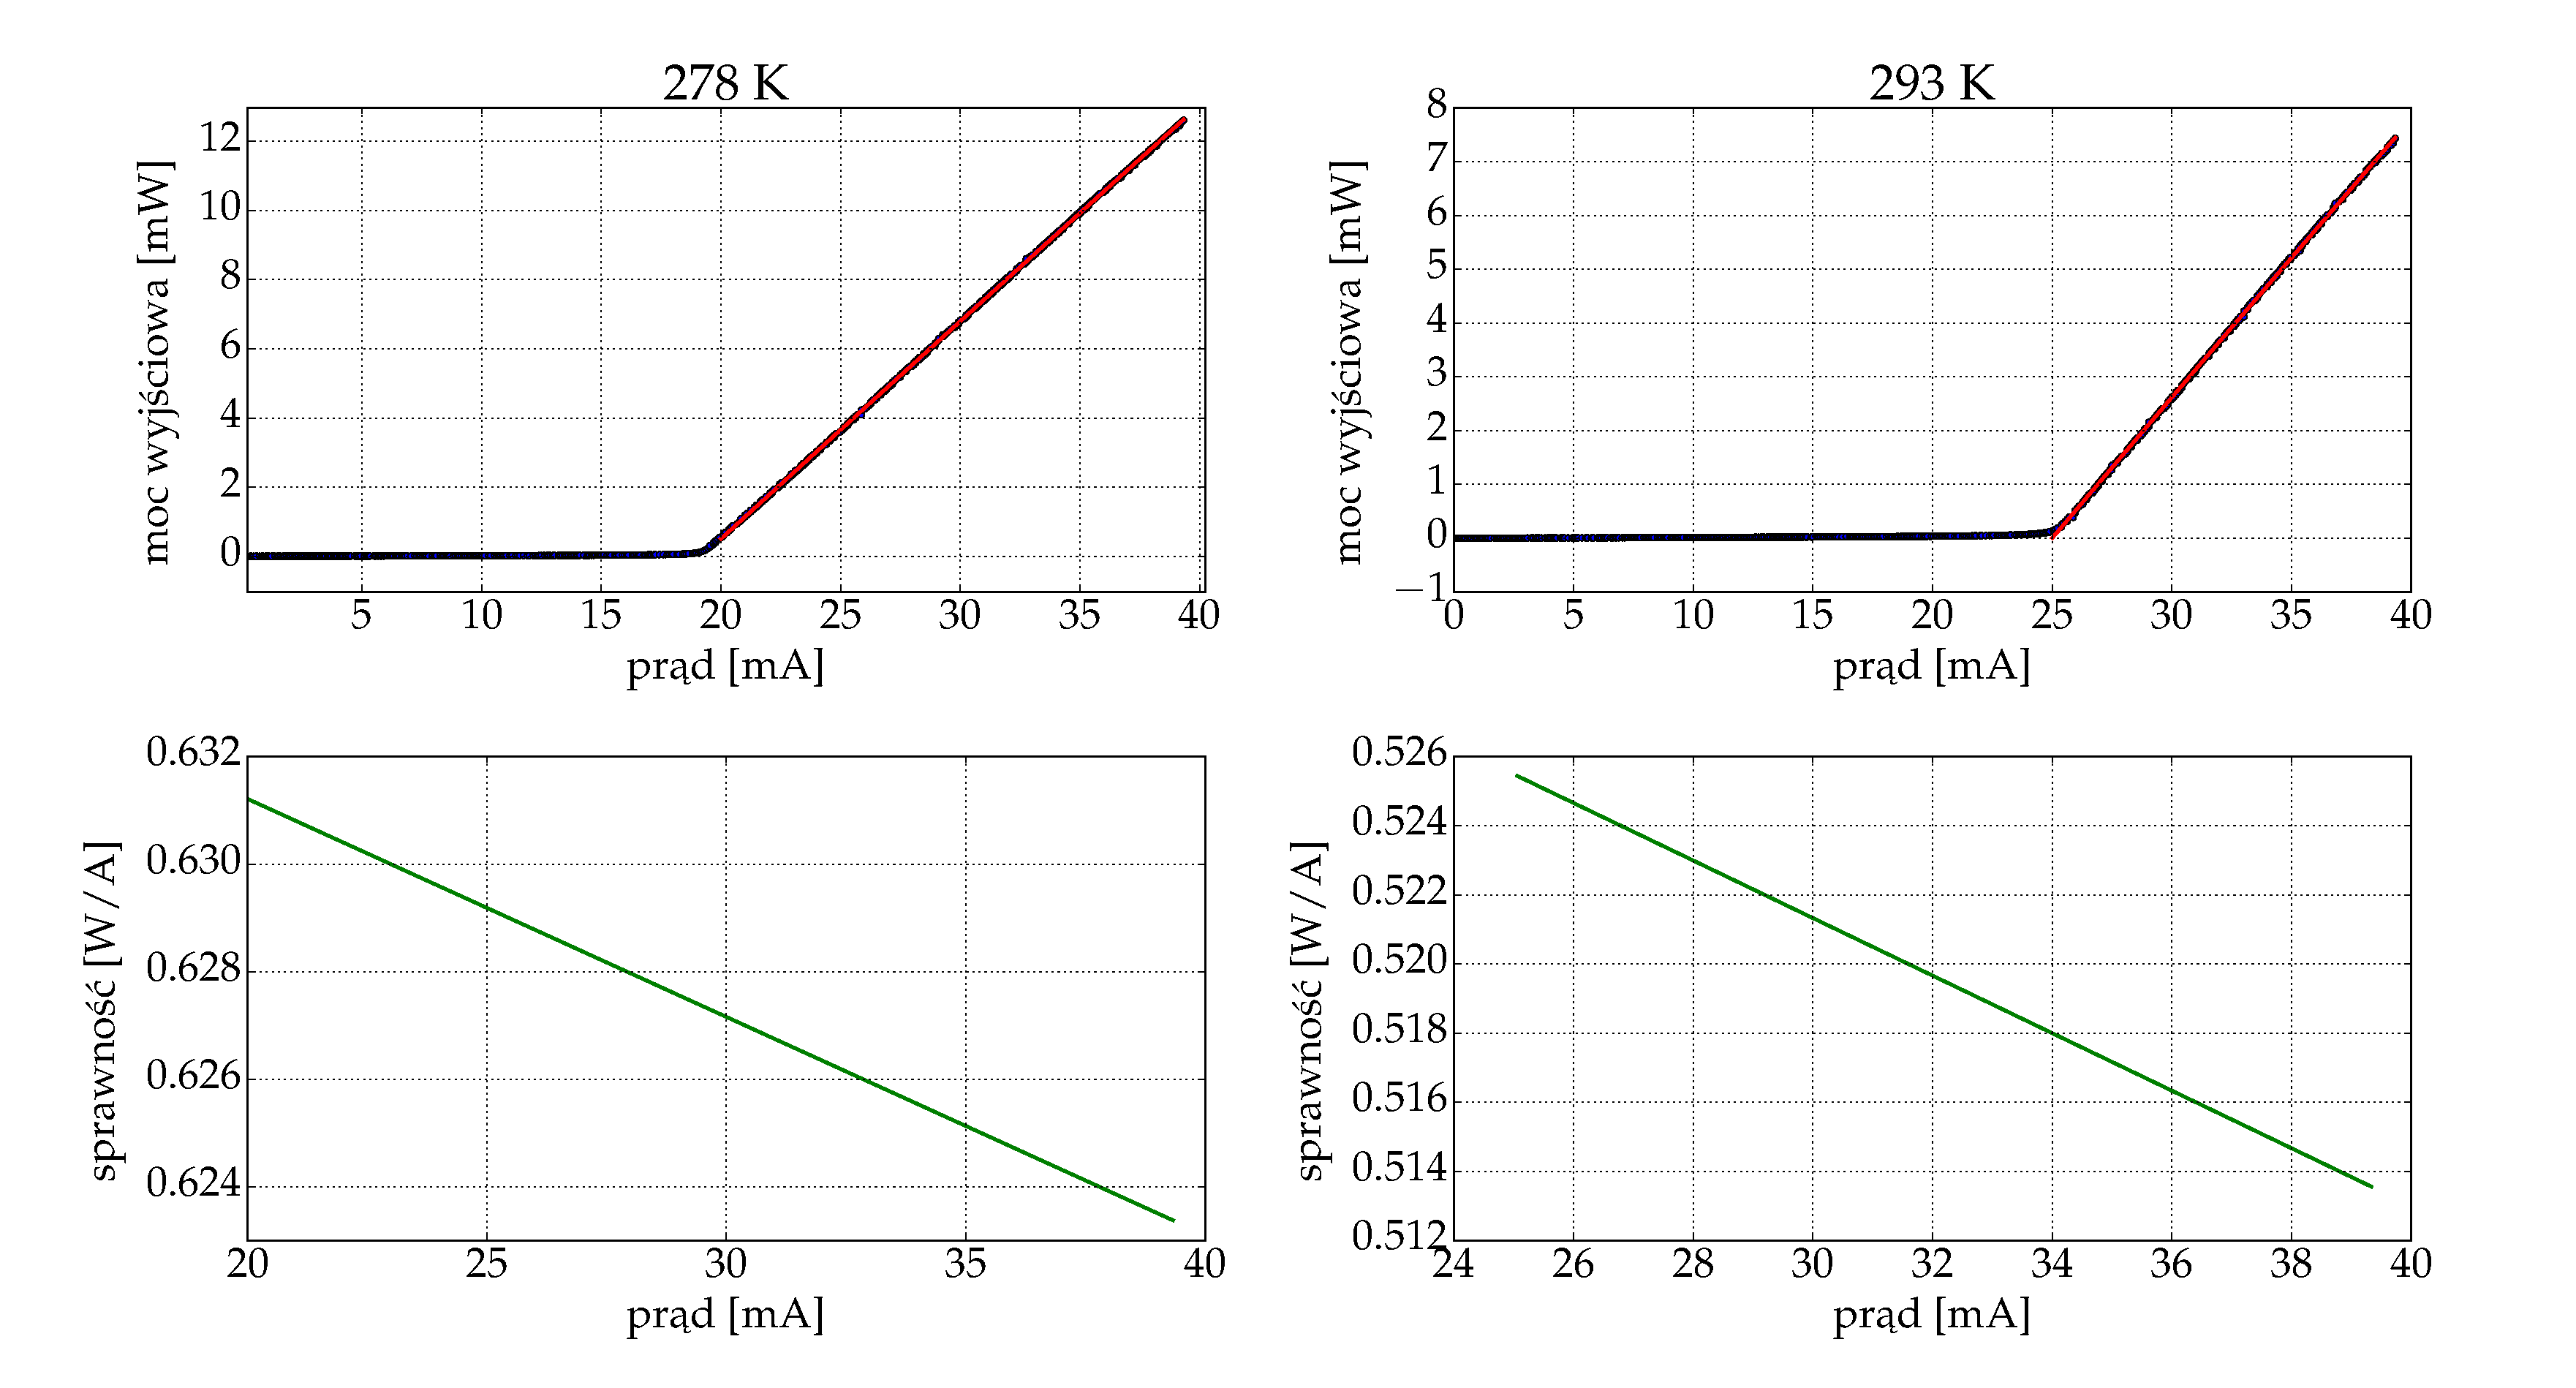
\includegraphics[scale=0.30]{plot635/plot_eff_via_current4.eps}
  \label{rys3}
  \caption{Wykres sprawności różniczkowej dla lasera krawędziowego 635\,nm dla dwóch temperatur.}
\end{figure}
\begin{figure}
\center
  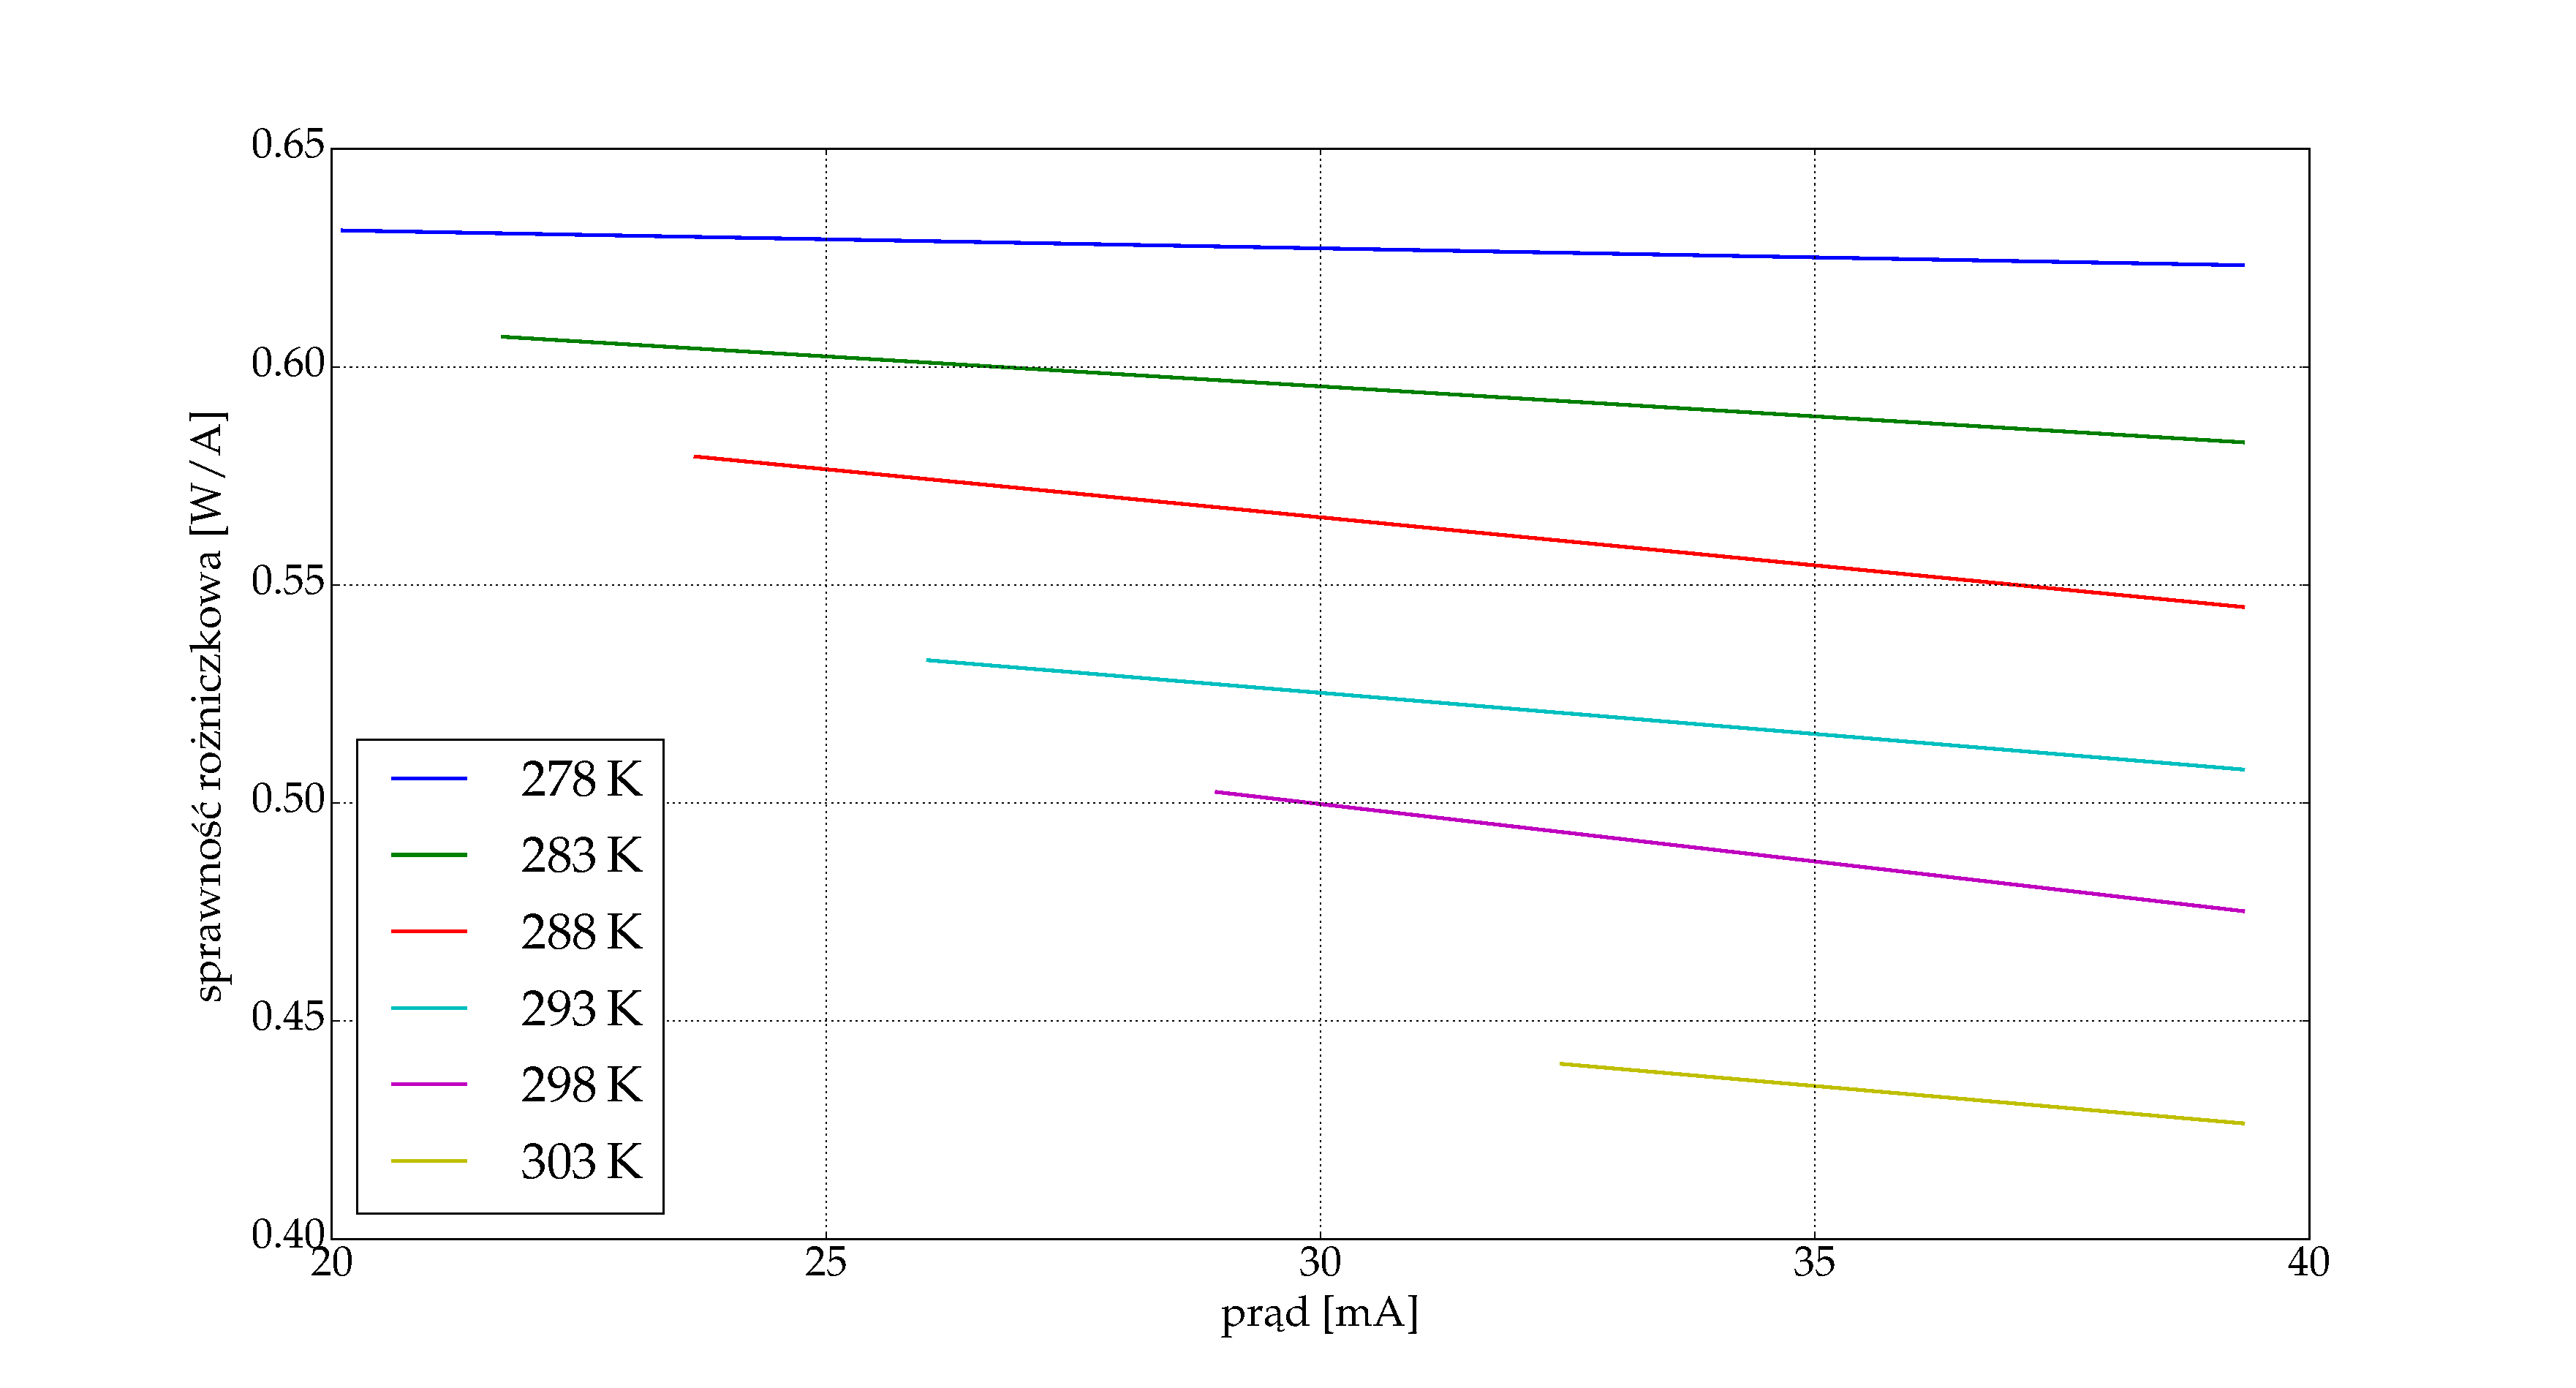
\includegraphics[scale=0.30]{plot635/plot_eff_via_current_all.eps}
  \label{rys3}
  \caption{Wykres sprawności w funkcji prądu dla lasera krawędziowego 635\,nm.}
\end{figure}
\newpage
\subsection{Laser krawędziowy 850\,nm (L850P010)--- omówienie wyników}
Pomiar przeprowadzany był w temperaturach chłodnicy od 283\,K do 353\,K z krokiem co 5\,K. Wartości wyznaczonego prądu progowego
znajdują się w tabeli~(\ref{tab:tabela850}). Rysunki od~(\ref{fig:plot_i_th4_850}) do~(\ref{fig:plot_wall_eff_850}) dotyczą lasera
krawędziowego 850\,nm.
\begin{itemize}
\item Wykres na rysunku~(\ref{fig:plot_i_th4_850}) przedstawia sposób, w jaki wyznaczana była wartość prądu progowego. Następnie na podstawie
wyznaczonych wartości w danej temperaturze sporządziłem wykres prądu progowego w zależności od temperatury
przedstawiony na rysunku~(\ref{fig:plot_fit_850}). Do wykreślonych wartości punktów dopasowałem funkcję~(\ref{eq:i_th}) w wyniku czego otrzymałem
temperaturę charakterystyczną, $T_0$, która wynosiła ($157 \pm 4$)\,K oraz parametr $I_0$, którego wartość wynosiła (1.7 $\pm$ 0.1)\,mA.
Porównująć wyznaczone wartości $T_0$ oraz $I_0$ dla lasera krawędziowego 850\,nm z wartościami dla lasera krawędziowego 635\,nm, należy
zauważyć, że wartości te są większe.
\item Analizując wykres napięcia na laserze od prądu wejściowego przedstawiony na rysunku~(\ref{fig:plot_i_v_i_l_850})
można zauważyć, że wraz ze wzrostem temperatury na chłodnicy
maleje opór lasera. Wraz ze wzrostem temperaturą chłodnicy maleje także moc wyjściowa lasera.
\item Wykres na rysunku~(\ref{fig:eff_via_current4_850}) przedstawia sprawność różniczkową lasera w funkcji prądu wejściowego
w różnych temperaturach chłodnicy. W górnej części rysunku pokazana jest zależność mocy wyjściowej od prądu, do której dopasowałem
funkcje kwadratową dla punktów leżących powyżej wartości prądu progowego. Dopasowana funkcja zbliżona jest do funkcji liniowej, przez co sprawność różniczkowa jest
prawie stała w funkcji prądu, jednakże jak wynika z wykresu im wyższa temperatura, tym sprawność różniczkowa lasera jest mniejsza, chodź zmiany na
są małe około 0.014\,W/A dla temperatury 353\,K przy zakresie prądu od 16.6\,mA do 80\,mA oraz 0.017\,W/A dla temperatury 293\,K
przy zakresie prądu od 11.1\,mA do 80\,mA.
\item Wykres na rysunku~(\ref{fig:plot_eff_via_current_all_850}) przedstawia, jak zmienia się sprawność lasera od temperatury chłodnicy.
Funkcje, które przedstawiają sprawność zostały wyznaczone analogicznie jak te przedstawione na rysunku~(\ref{fig:eff_via_current4_850}).
Analizując ten wykres, dochodzę do wniosku, że wraz z wyższą temperaturą sprawność różniczkowa lasera maleje dla prądu wejściowego powyżej
30\,mA. Dla mniejszych wartości prądu dla temperatur 323\,K oraz 333\,K jest inaczej, różnica ta jest niewielka i może być spowodowana błędem
wynikającym z metody najmniejszych kwadratów podczas dopasowywania funkcji~(\ref{eq:fit_i_th}).
\item Wykres na rysunku~(\ref{fig:plot_wall_eff_850}) przedstawia sprawność całkowitą lasera w funkcji prądu. Jak widzimy,
wraz ze wzrostem temperatury sprawność całkowita spada, choć spadek nie jest tak duży jak w przypadku lasera krawędziowego 635\,nm.
\end{itemize}
\begin{table}[H]
\begin{center}
\caption{ Wyznaczone wartości prądu progowego $I_{\mathrm{th}}$ w różnych temperaturach $T$ dla lasera krawędziowego 850\,nm.}
\begin{tabular}{ | C{1.5cm}|  C{3.0cm} | C{1.5cm} | C{3.0cm}| C{1.5cm} | C{3.0cm}|}
\hline
$T$ [K] &   $I_{\mathrm{th}}$ [mA]  &  $T$ [K] &   $I_{\mathrm{th}}$ [mA]  &  $T$ [K] &   $I_{\mathrm{th}}$ [mA] 	\\ \hline
283      &   10.48 $\pm$ 0.09  & 288      &   10.9 $\pm$ 0.1       & 293		 &   11.1 $\pm$ 0.1  \\ \hline
298		 &   11.33 $\pm$ 0.05  & 303		 &   11.65 $\pm$ 0.06  & 308		 &   11.98 $\pm$ 0.07  \\ \hline
313		 &   12.34 $\pm$ 0.07  & 318		 &   12.71 $\pm$ 0.08  & 323		 &   13.11 $\pm$ 0.09  \\ \hline
328		 &   13.57 $\pm$ 0.07  & 333		 &   14.1 $\pm$ 0.1    & 338		 &   14.6 $\pm$ 0.1  \\ \hline
343		 &   15.2 $\pm$ 0.2    & 348		 &   15.7 $\pm$ 0.2    & 353		 &   16.6 $\pm$ 0.2  \\ \hline
\end{tabular}
\label{tab:tabela850}
\end{center}
\end{table}
\begin{figure}[H]
\center
  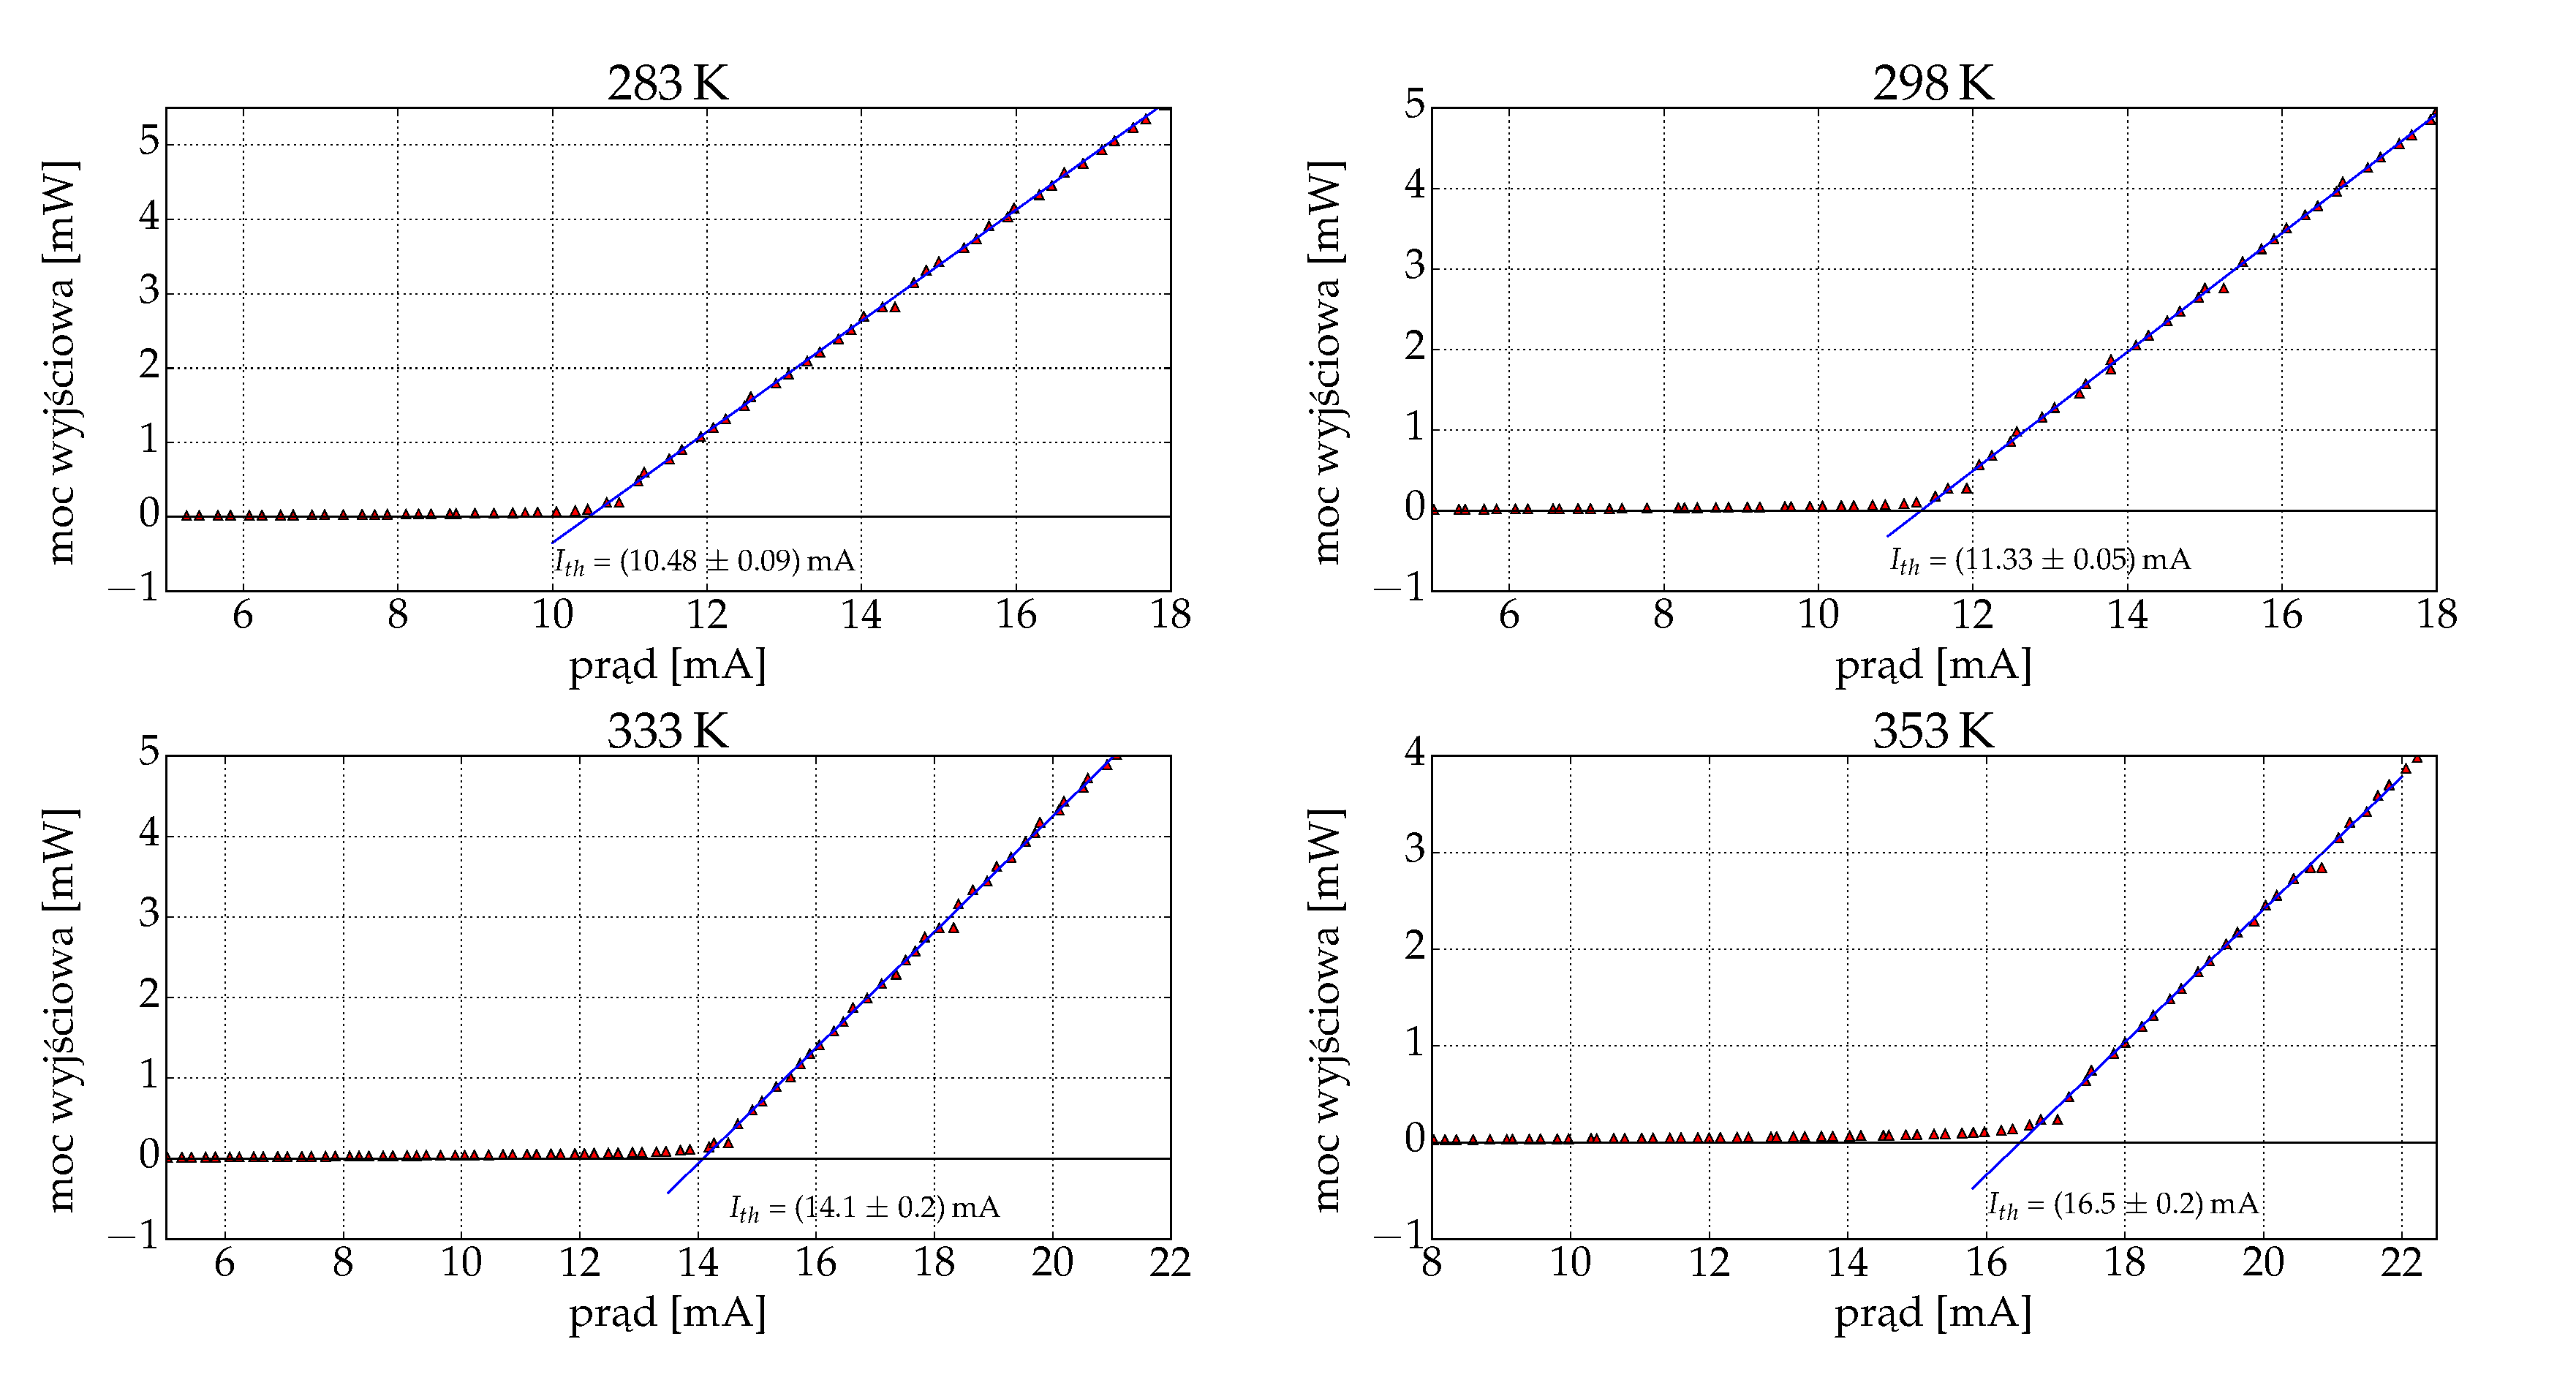
\includegraphics[scale=0.30]{plot_edge_850/plot_i_th4.eps}
  \label{rys1}
  \caption{Wykres ilustrujący wyznaczanie prądu progowego dla lasera krawędziowego 850\,nm.}
  \label{fig:plot_i_th4_850}
\end{figure}
\begin{figure}
\center
  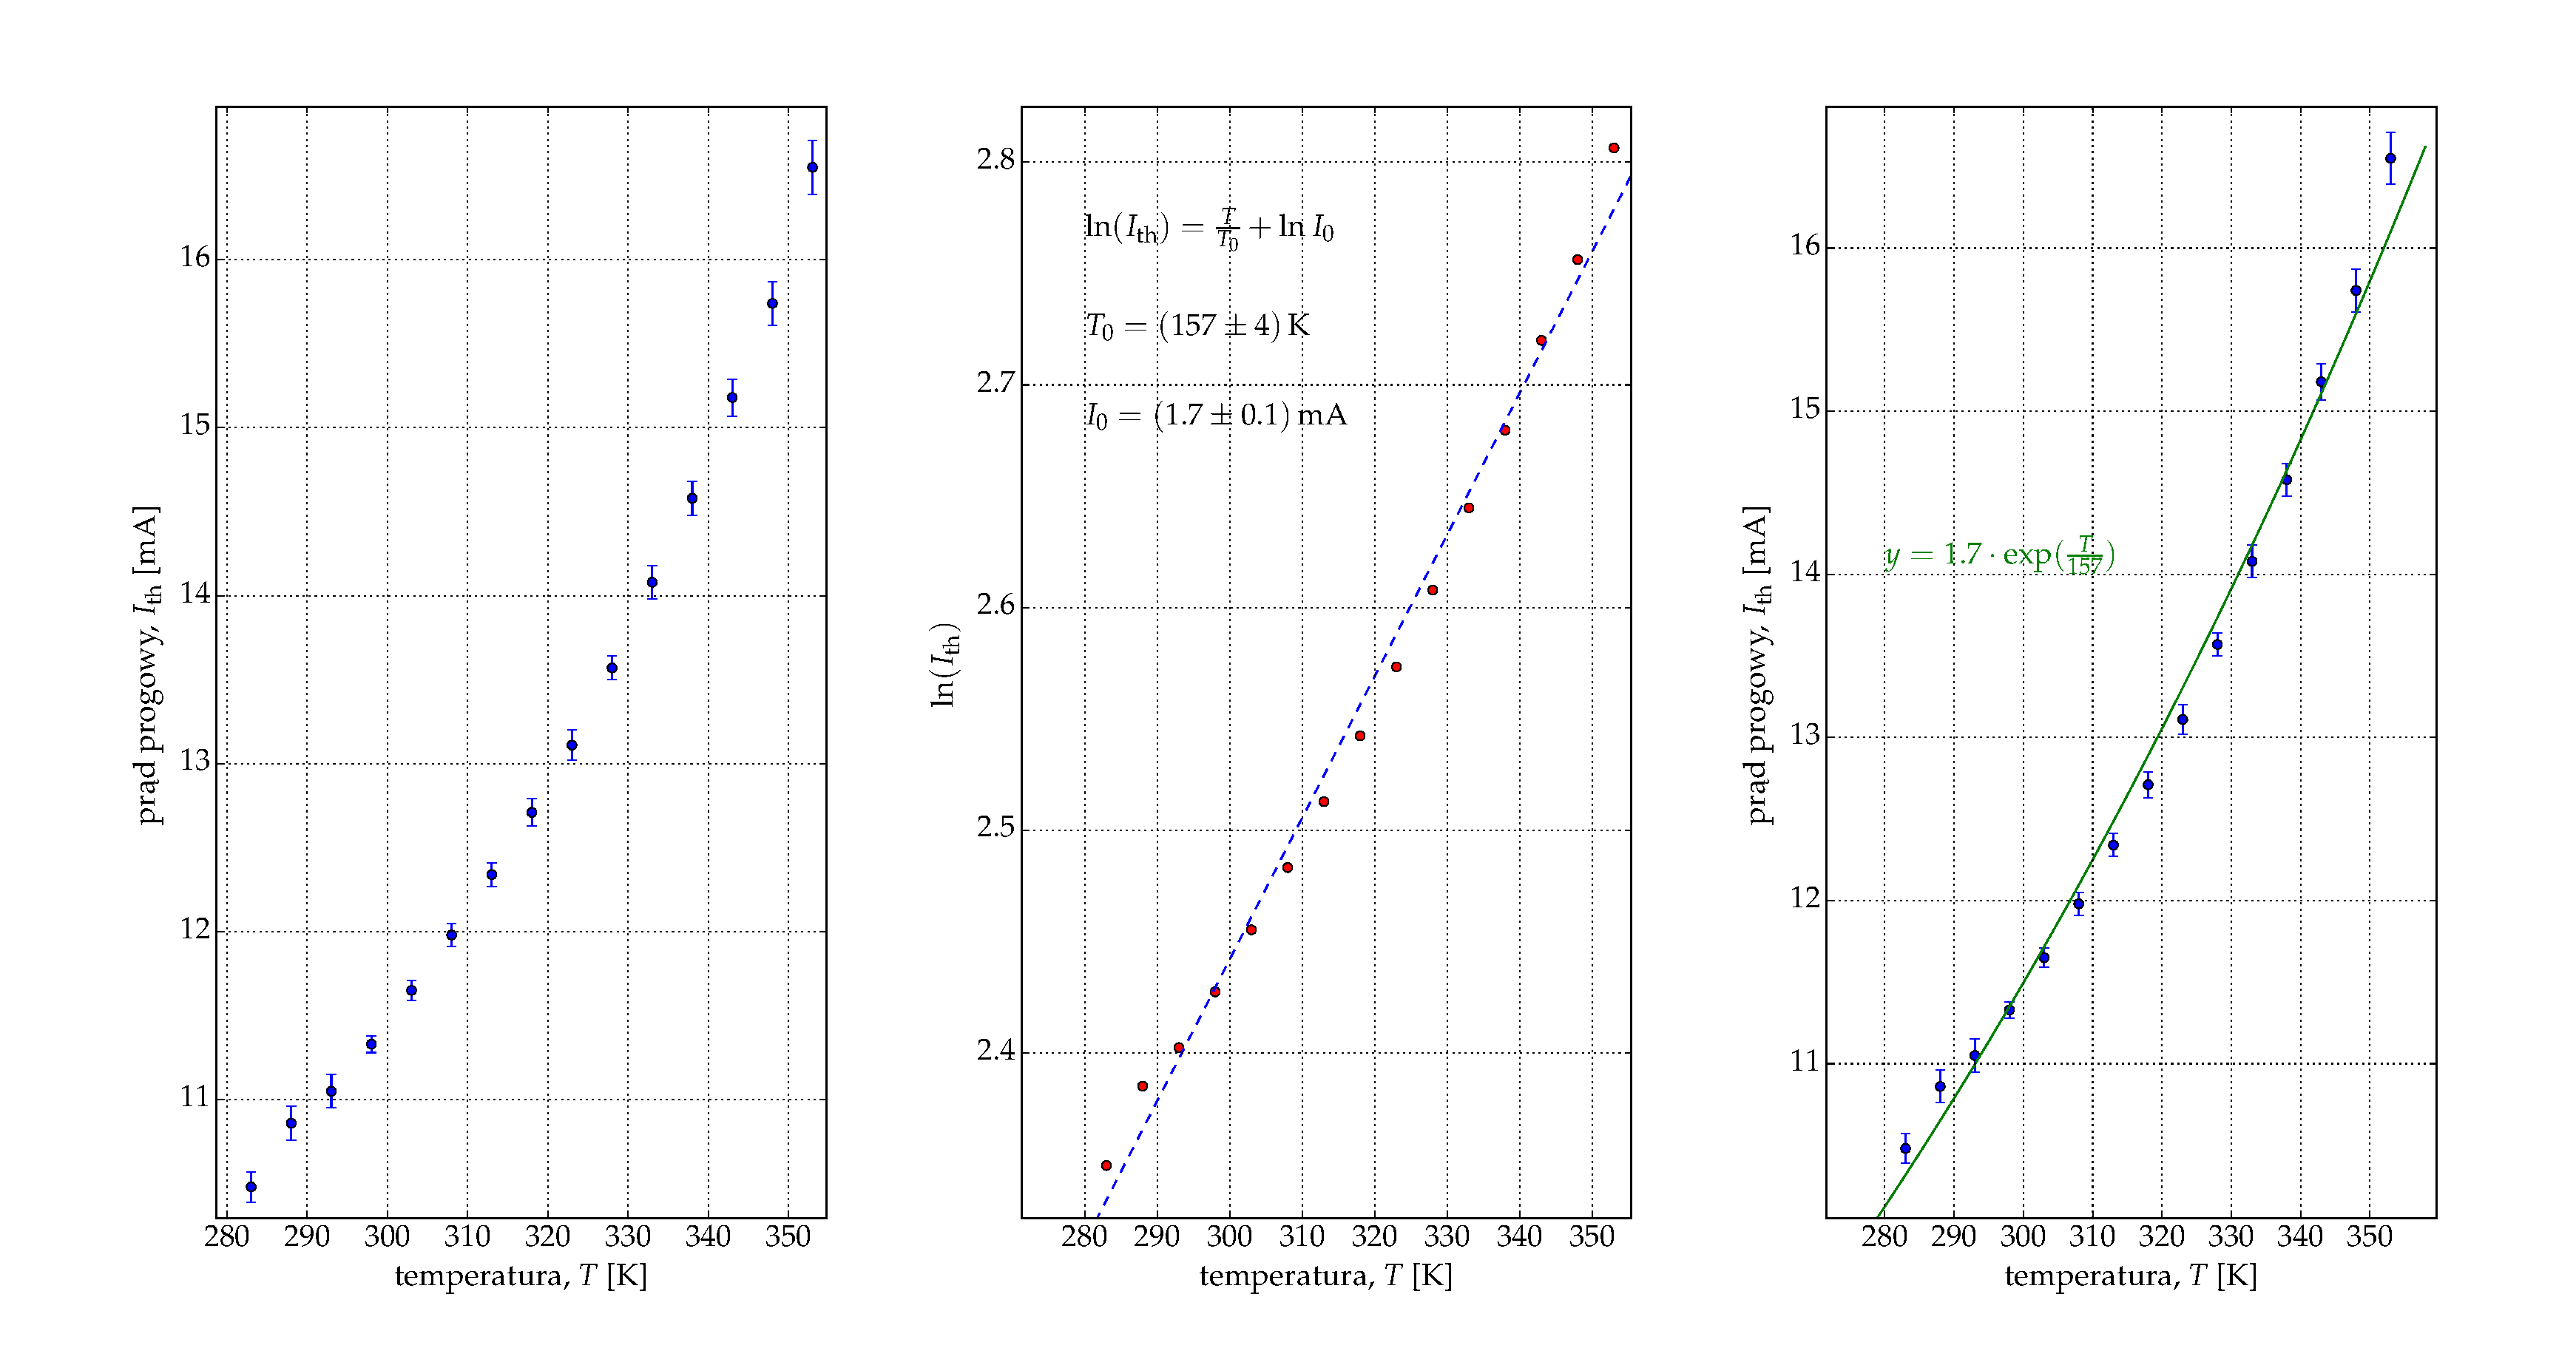
\includegraphics[scale=0.30]{plot_edge_850/plot_fit.eps}
  \label{rys1}
  \caption{Wykres prądu progowego w zależności od temperatury chłodnicy z dopasowanymi wartościami $I_{0}$ i $T_{0}$ dla lasera krawędziowego 850\,nm.}
  \label{fig:plot_fit_850}
\end{figure}
\begin{figure}
\center
  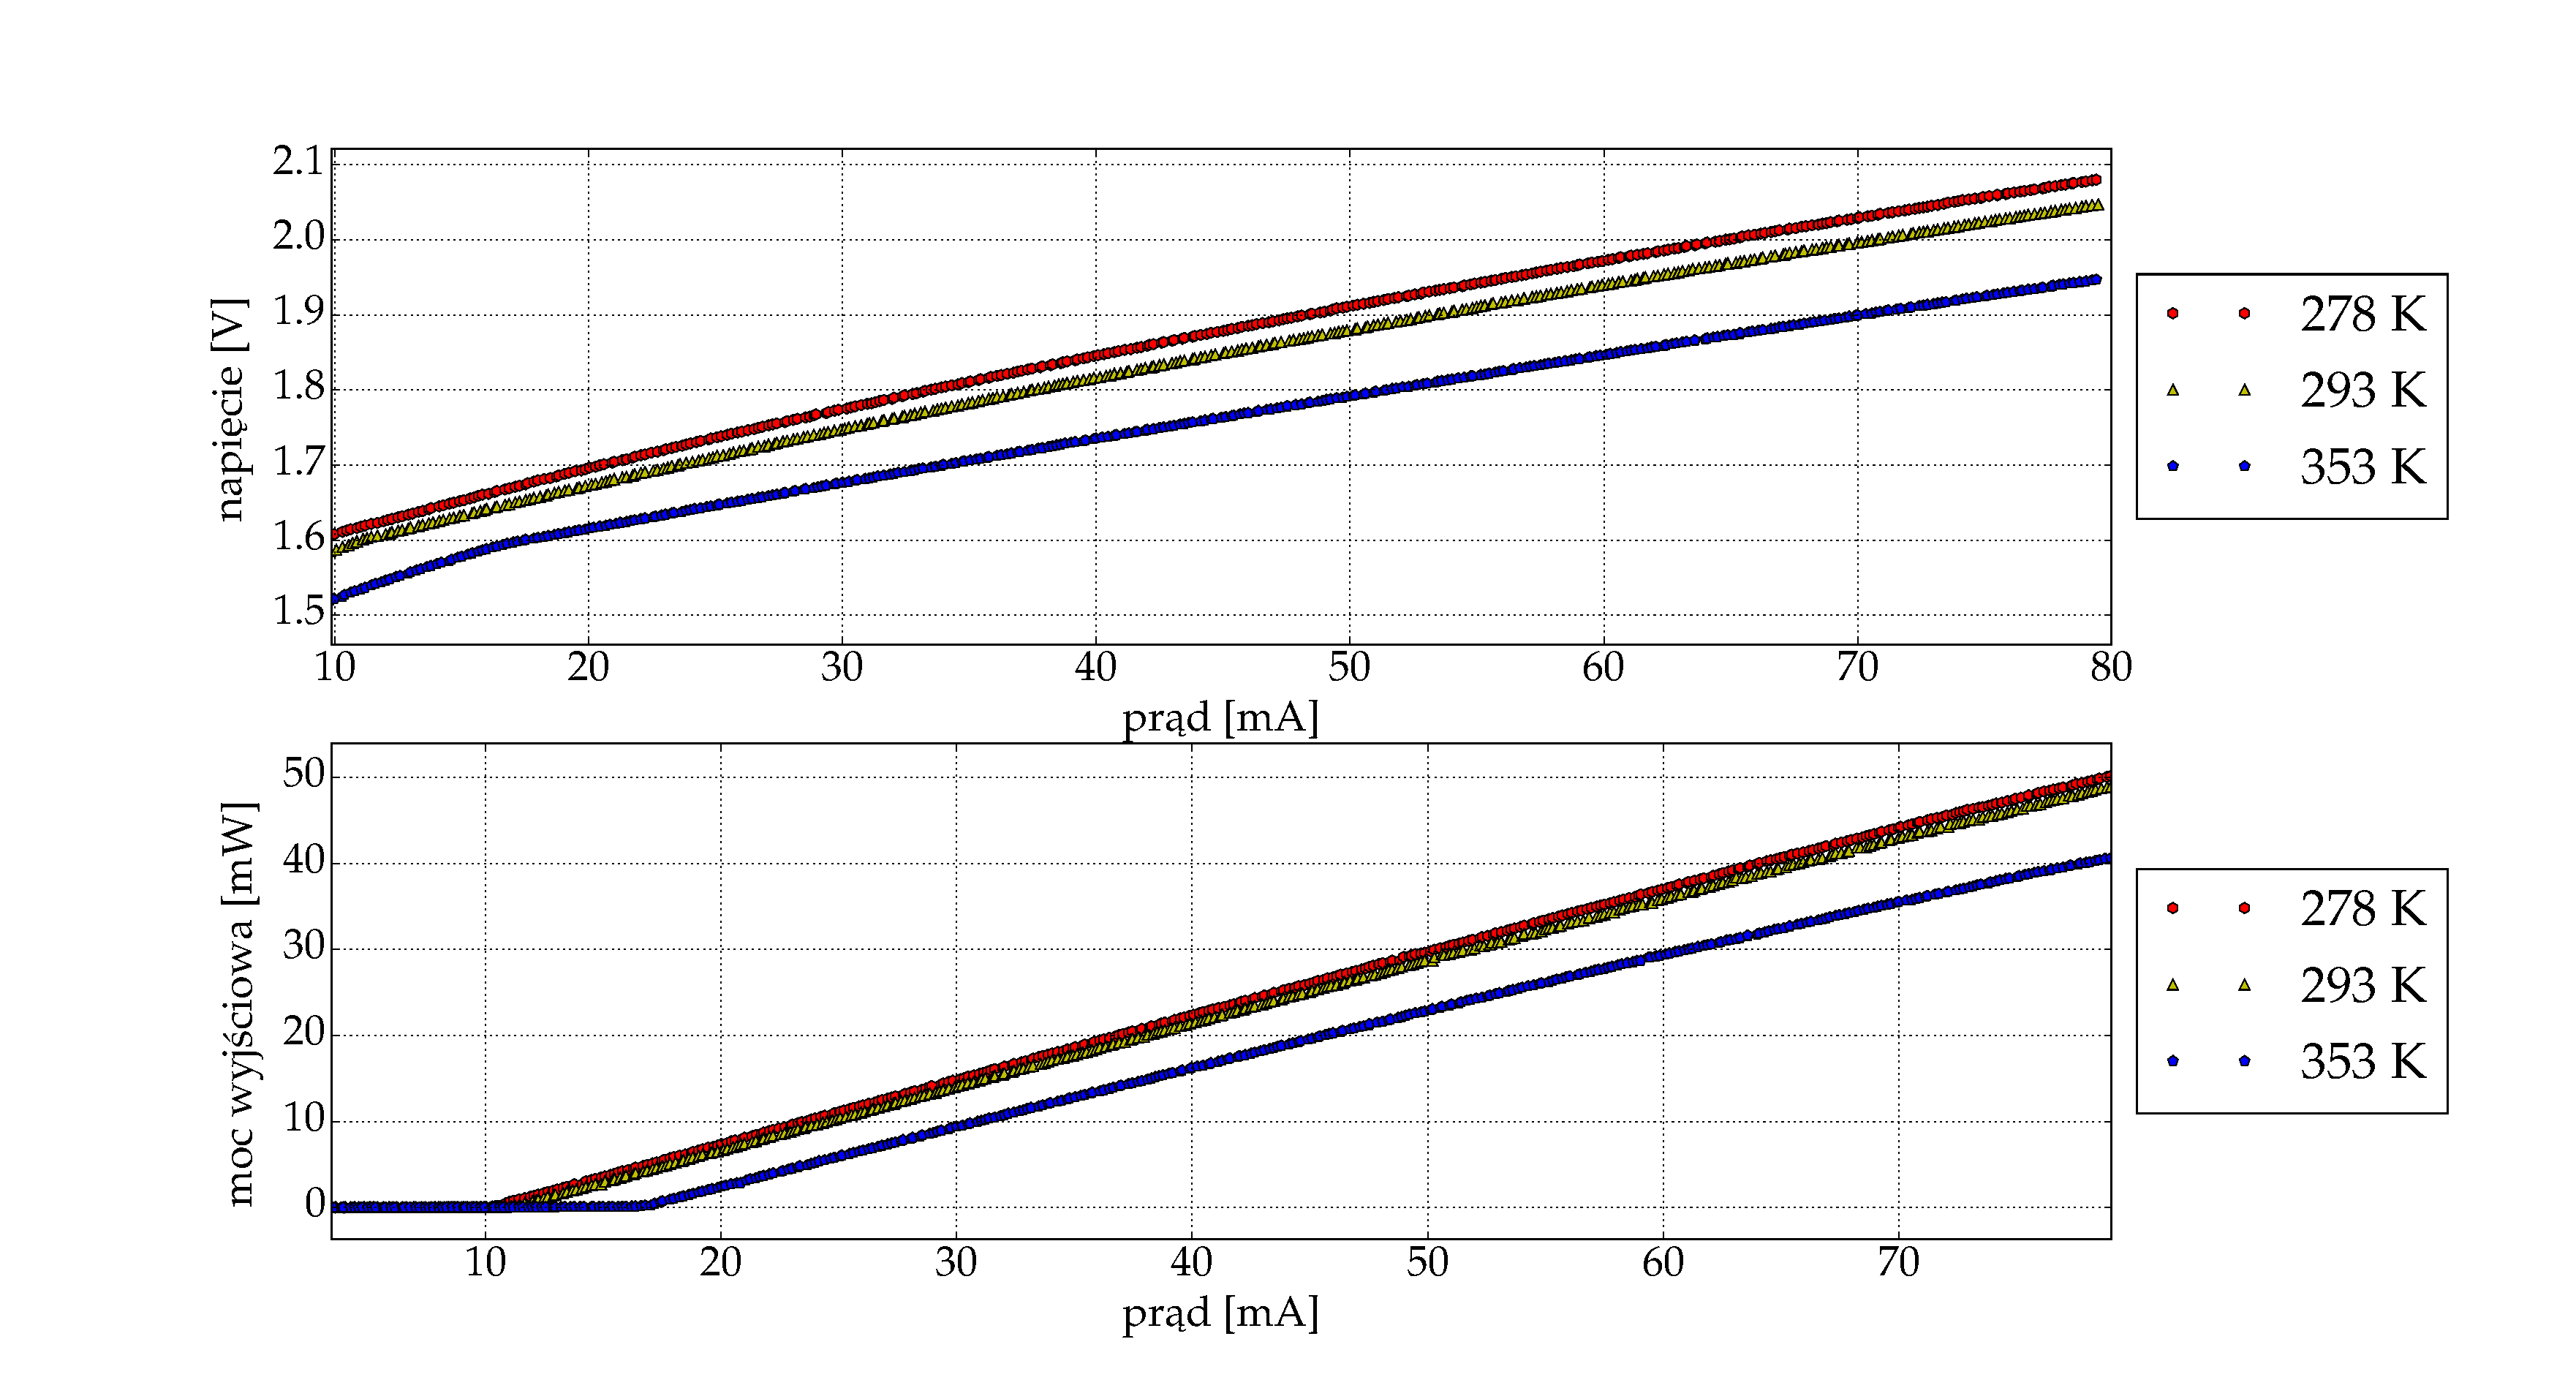
\includegraphics[scale=0.30]{plot_edge_850/plot_i_v_i_l.eps}
  \label{rys1}
  \caption{Wykres napiięcia oraz mocy wyjściowej w funkcji prądu dla lasera krawędziowego 850\,nm w różnych temperaturach.}
  \label{fig:plot_i_v_i_l_850}
\end{figure}
\begin{figure}
\center
  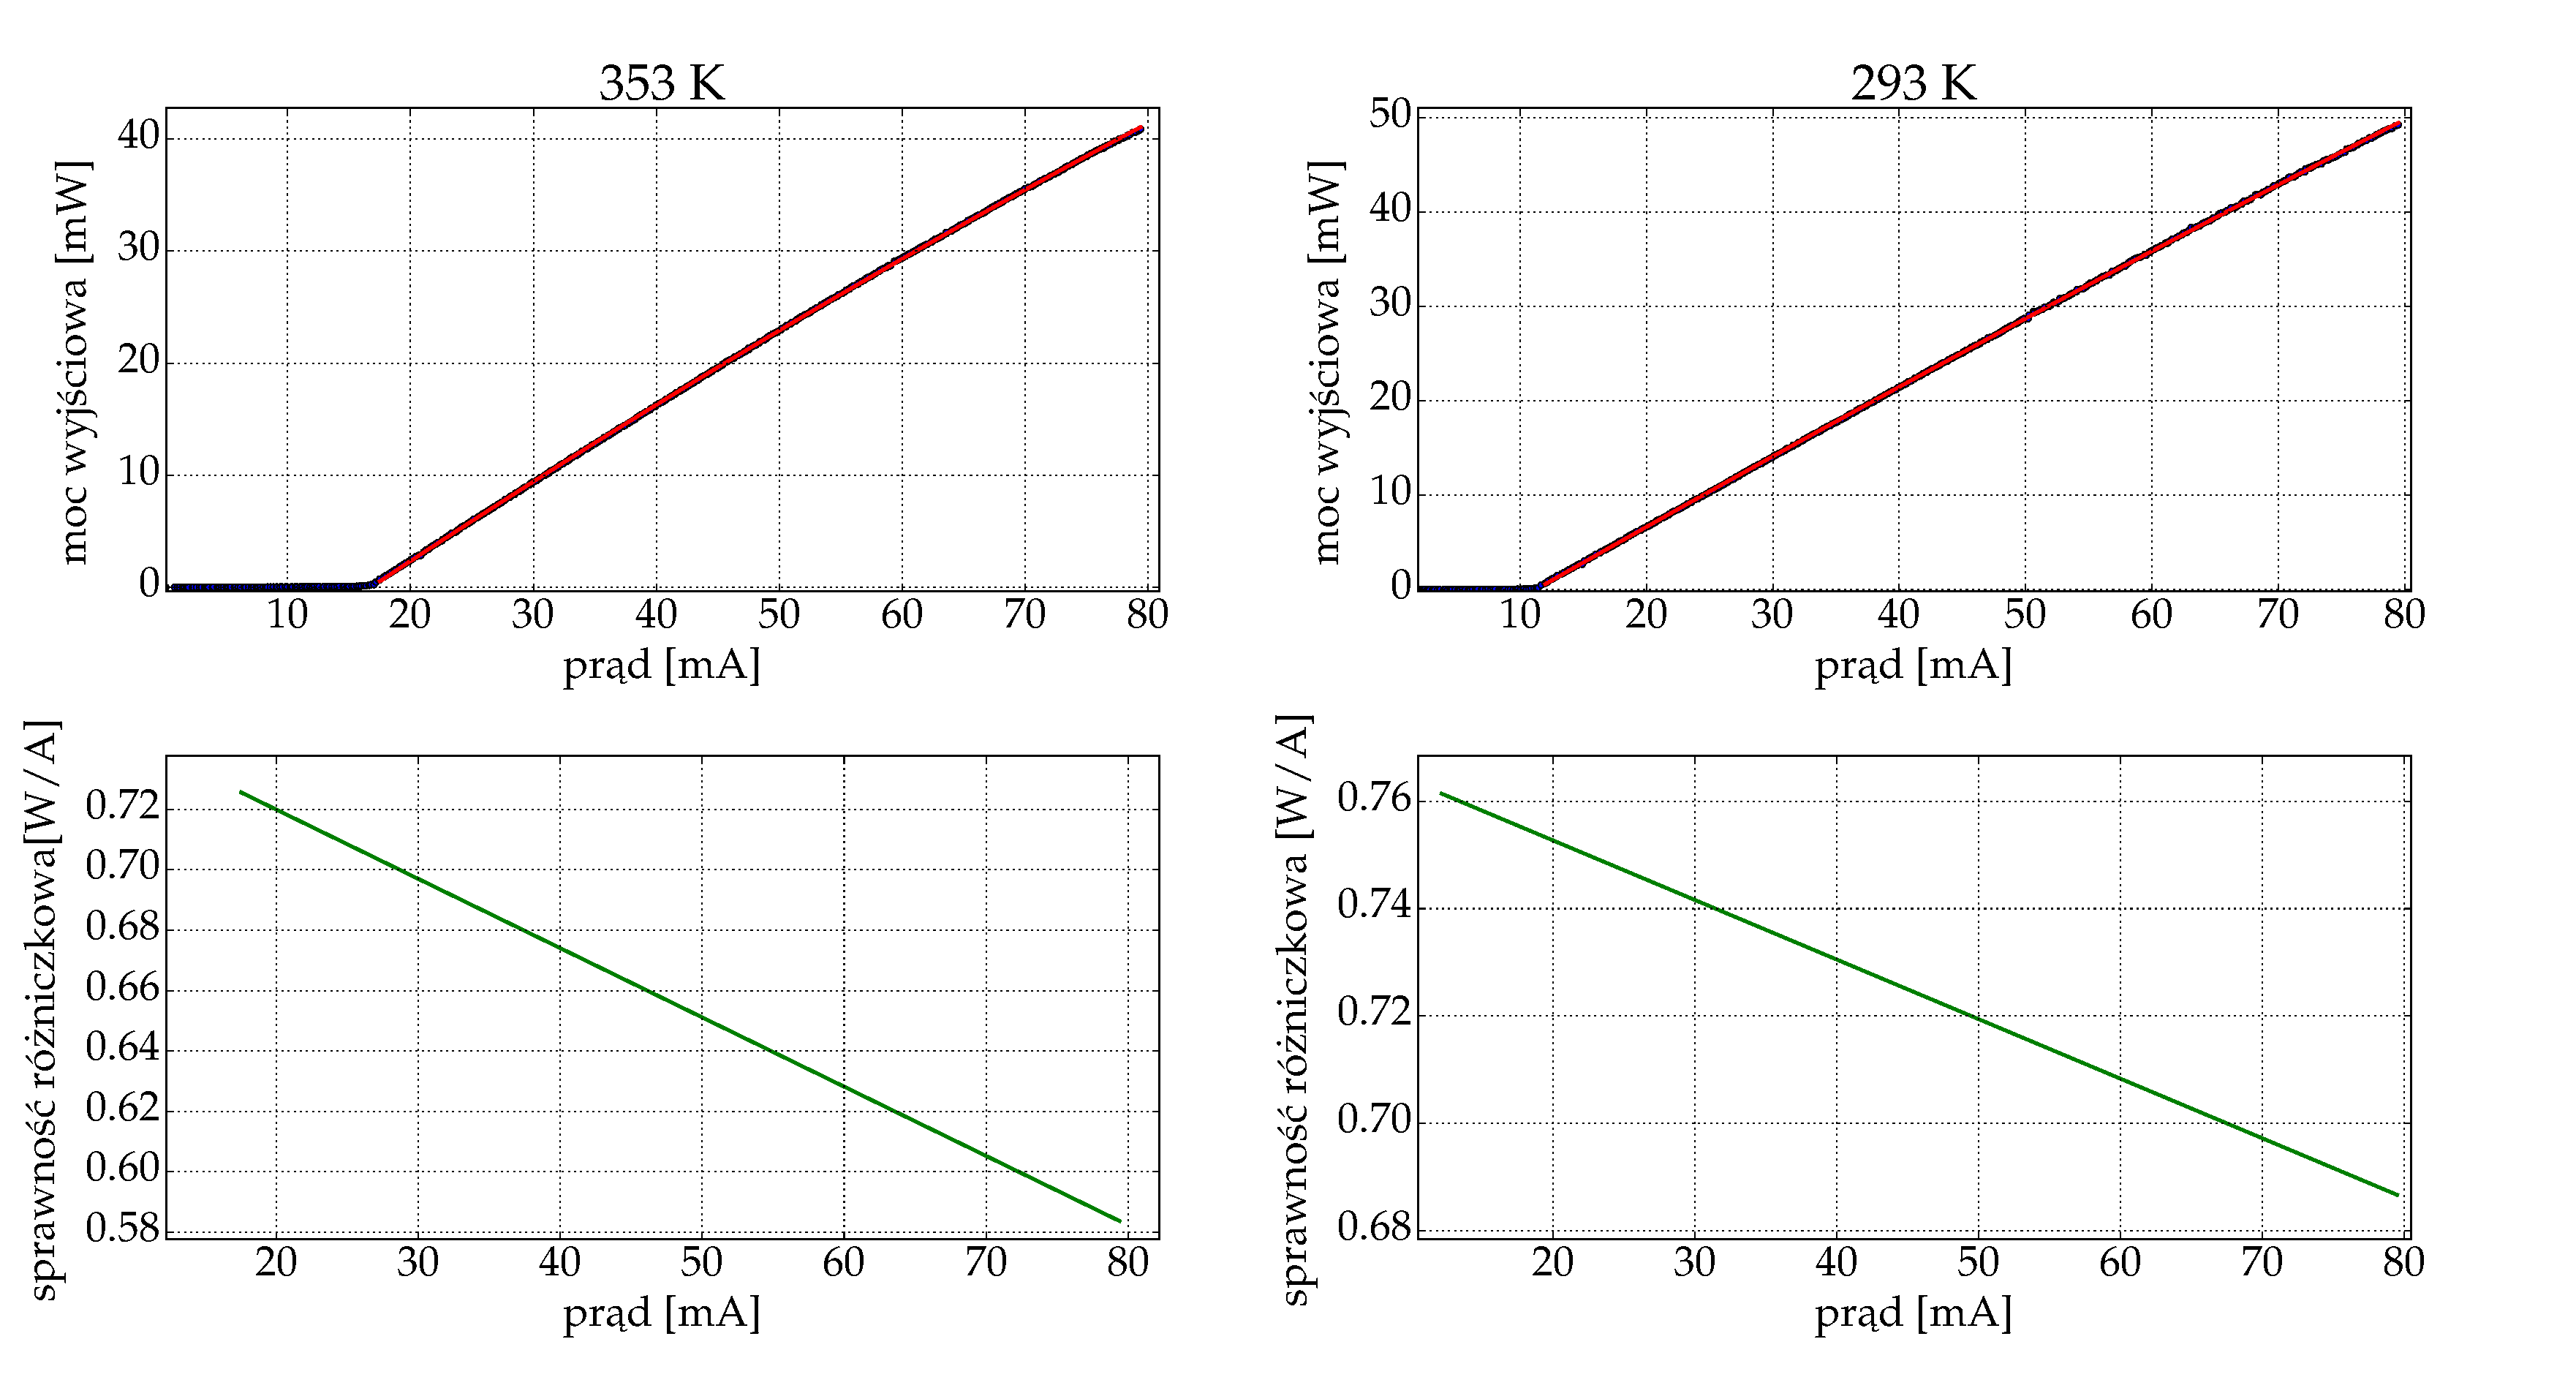
\includegraphics[scale=0.30]{plot_edge_850/eff_via_current4.eps}
  \label{rys1}
  \caption{Wykres sprawności różniczkowej dla lasera krawędziowego 850\,nm dla dwóch temperatur. U góry dopasowana funkcja,
u dołu pochodna tej funkcji reprezentująca sprawność różniczkową.}
  \label{fig:eff_via_current4_850}
\end{figure}
\begin{figure}
\center
  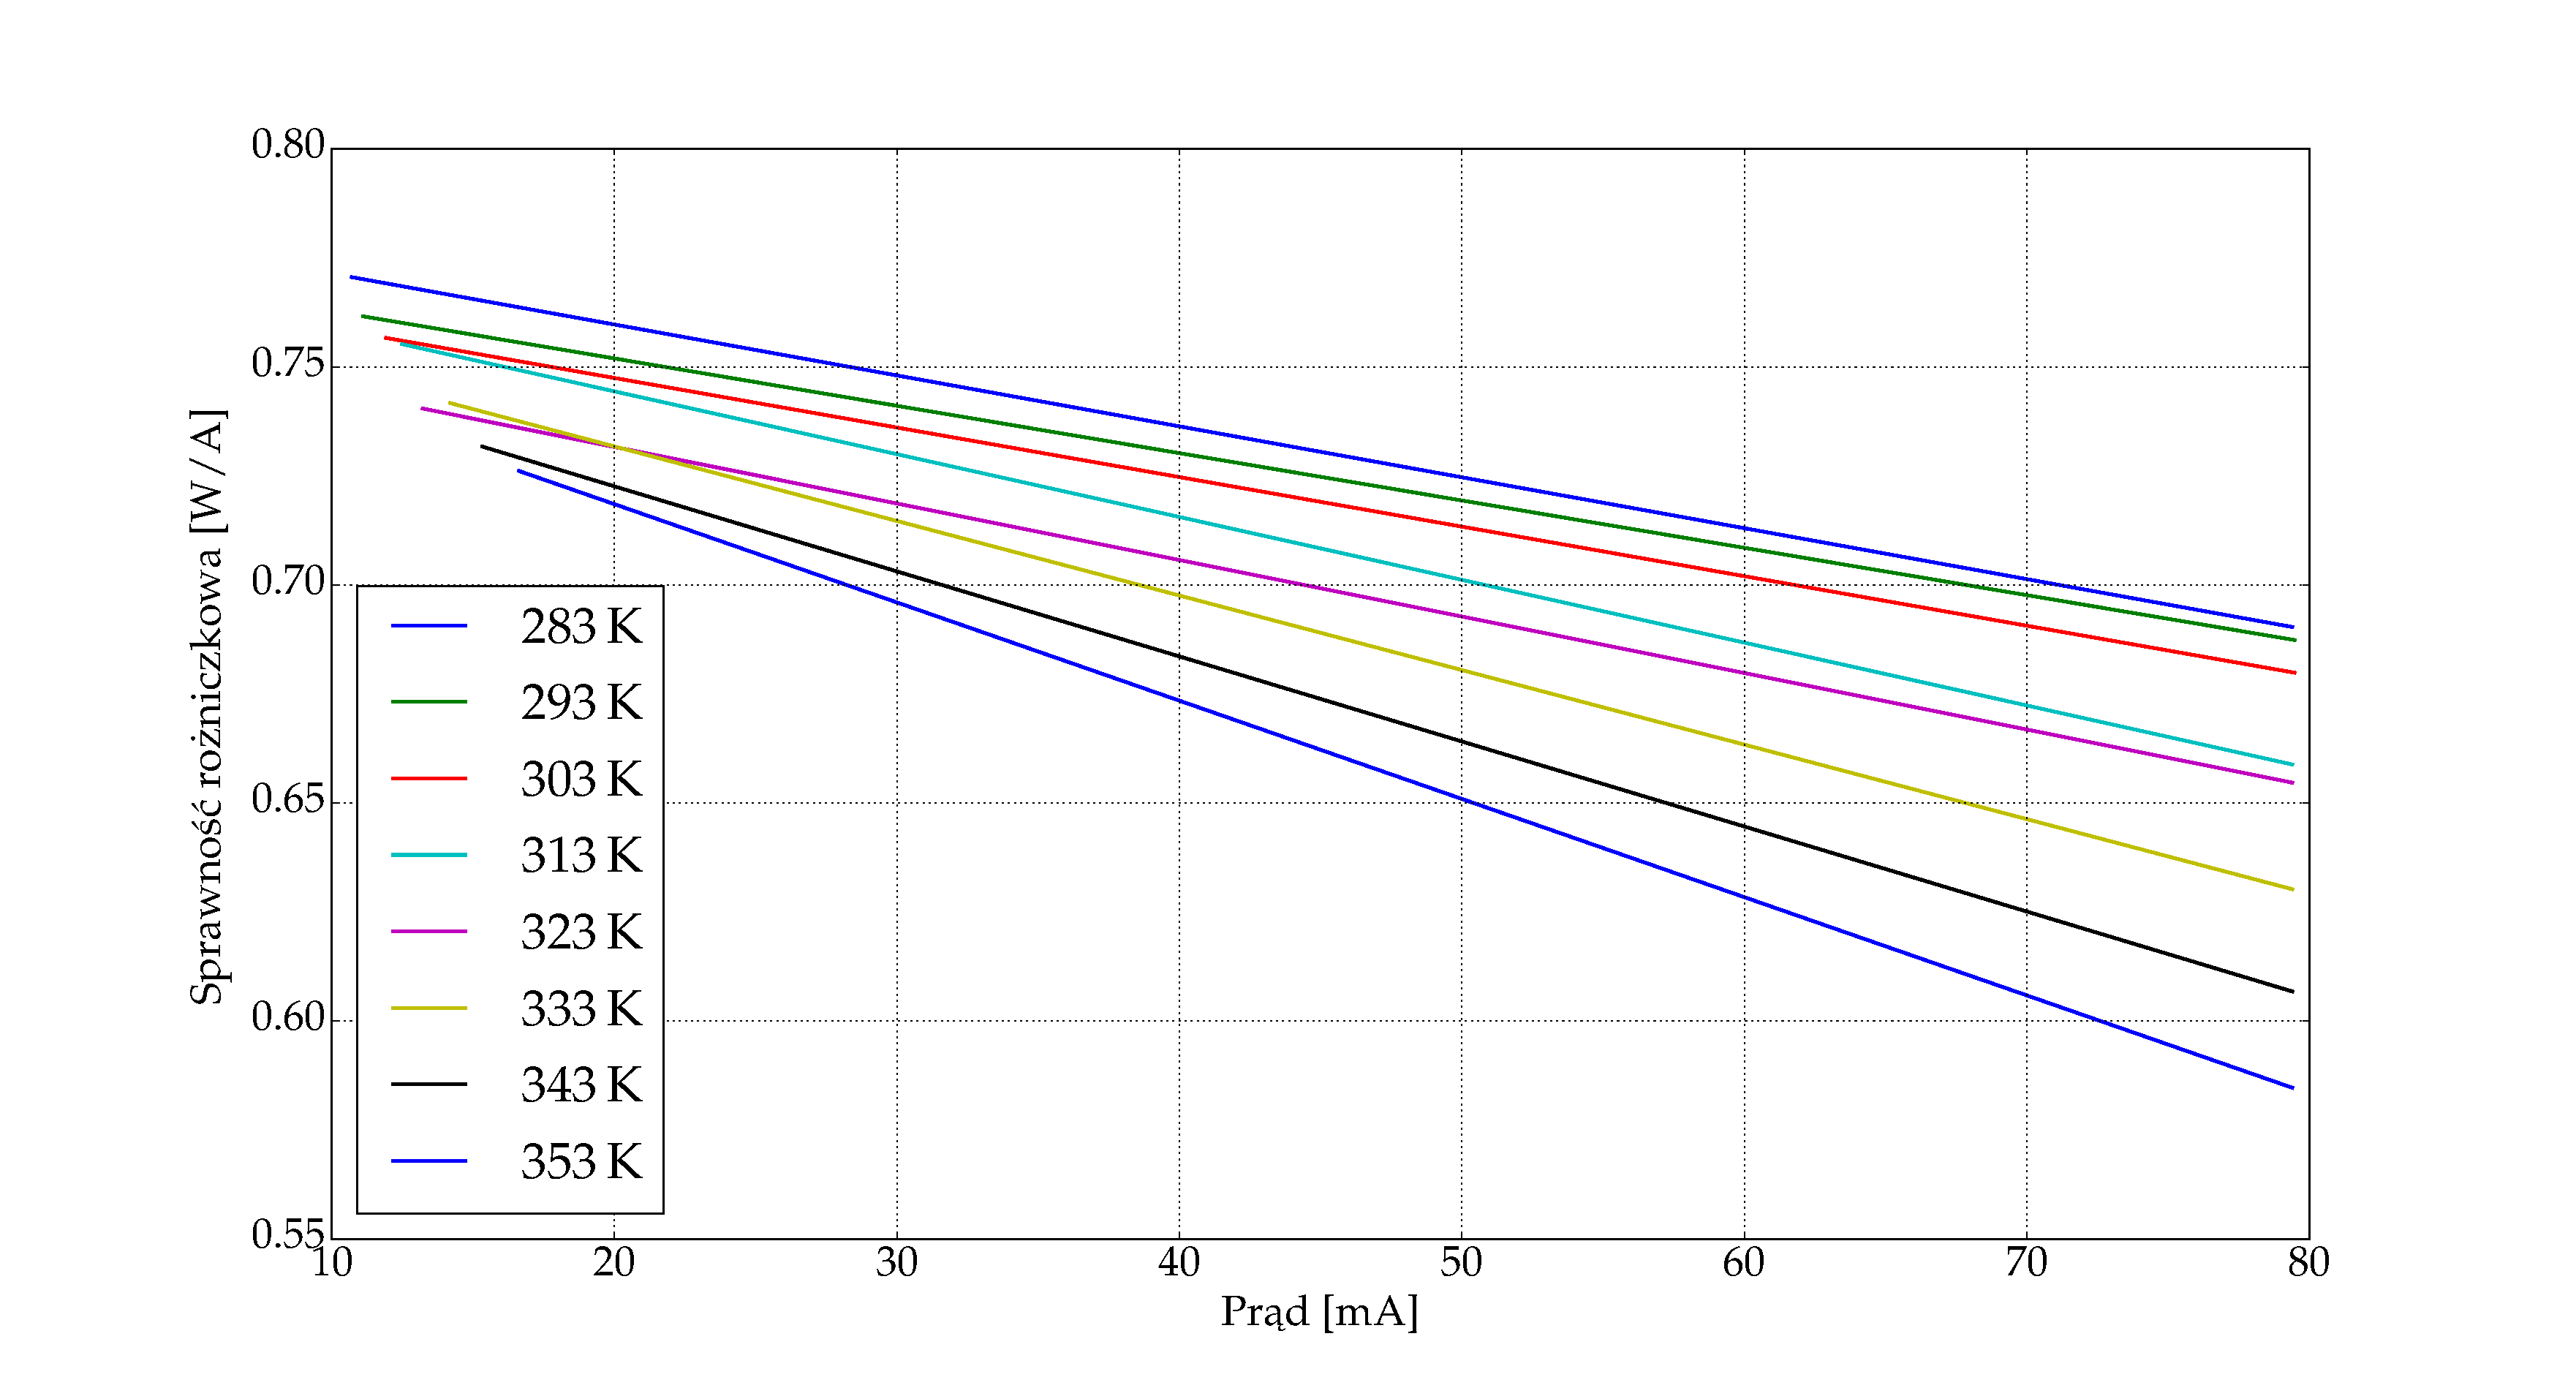
\includegraphics[scale=0.25]{plot_edge_850/plot_eff_via_current_all.eps}
  \label{rys1}
  \caption{Wykres sprawności różniczkowej dla lasera krawędziowego 850\,nm w różnych temperaturach.}
  \label{fig:plot_eff_via_current_all_850}
\end{figure}
\begin{figure}
\center
  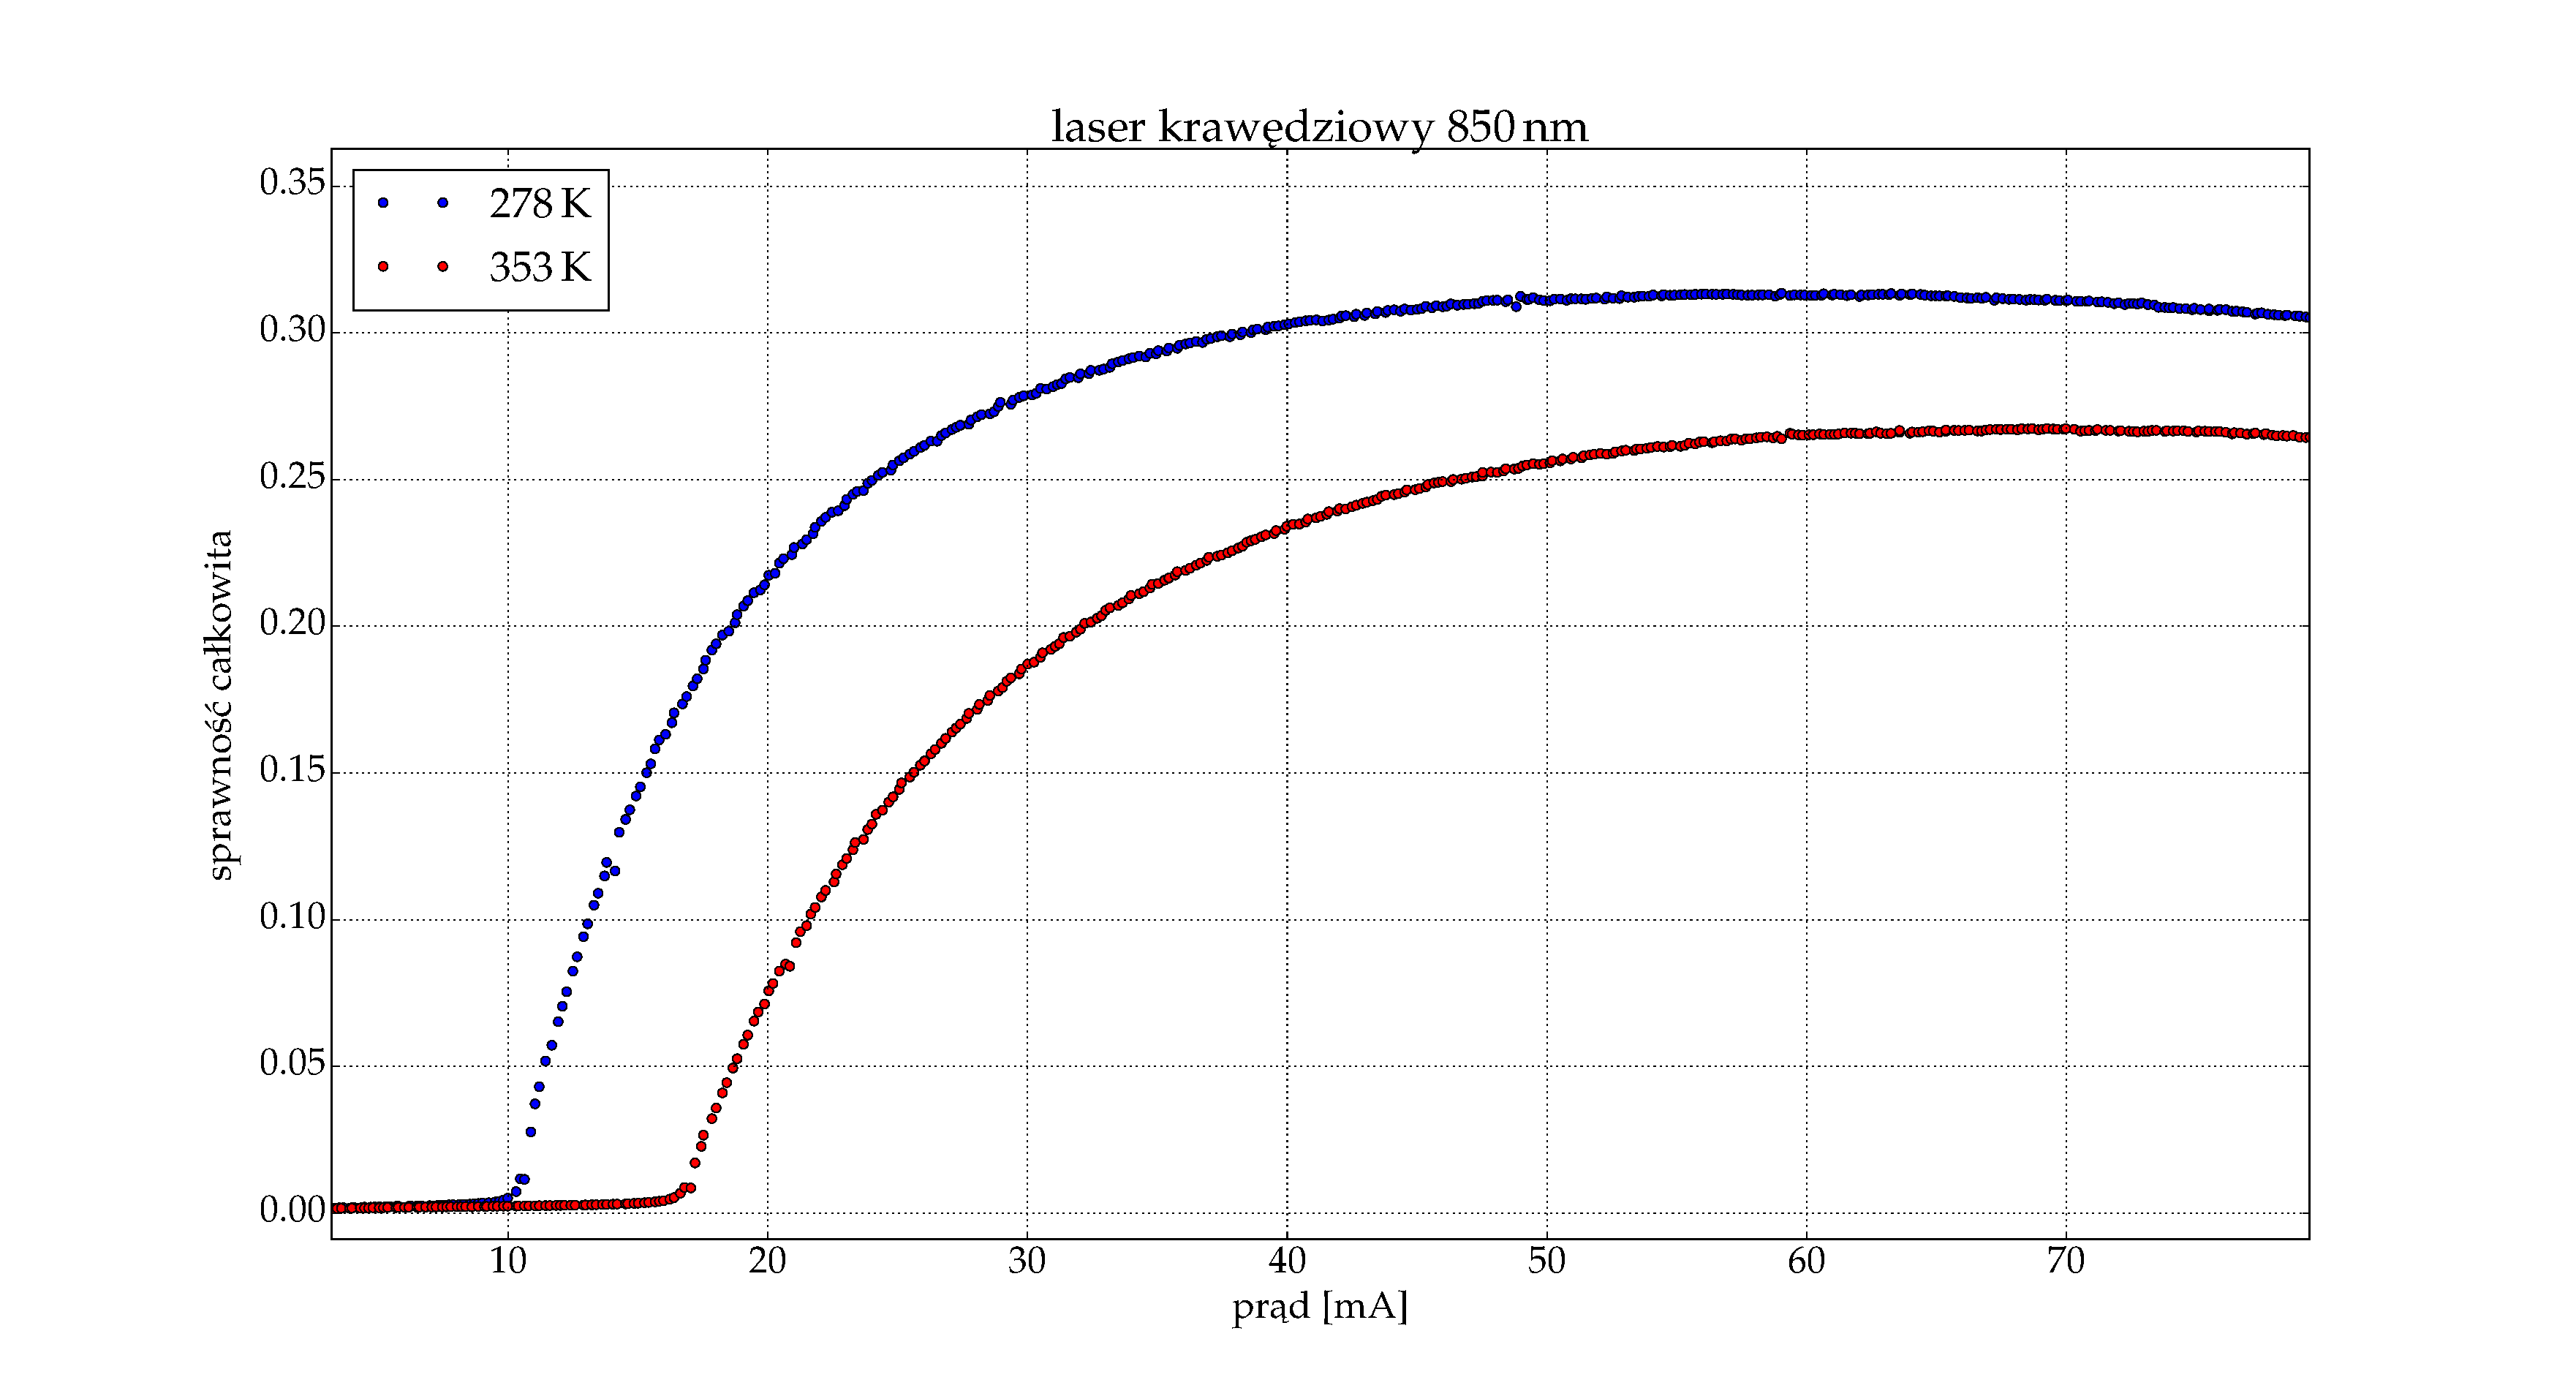
\includegraphics[scale=0.25]{plot_edge_850/plot_wall_eff.eps}
  \label{rys1}
  \caption{Wykres sprawności całkowitej w funkcji prądu dla lasera krawędziowego 850\,nm dla dwóch temperatur.}
  \label{fig:plot_wall_eff_850}
\end{figure}
\newpage
\newpage
\newpage
\subsection{Laser VCSEL 850\,nm --- omówienie wyników}
Pomiar przeprowadzany był w temperaturach chłodnicy od 283\,K do 353\,K, krokiem co 5\,K. Wartości wyznaczonego prądu progowego
znajdują się w tabeli~\ref{tab:tabela_vcsel850}. Rysunki od ~\ref{fig:plot_fit_i_th_vcsel850} do ~\ref{fig:plot_eff_all_via_current_vcsel850} dotyczą lasera
VCSEL 850\,nm.
\begin{itemize}
\item Wykres na rysunku~\ref{fig:plot_fit_i_th_vcsel850} przedstawia sposób wyznaczana wartość prądu progowego. Następnie na podstawie
wyznaczonych wartości w danej temperaturze, sporządziłem wykres prądu progowego w zależności od temperatury
przedstawiony na rysunku~\ref{fig:plot_temp_i_th_log_lin_vcsel850}. Jak widzimy, wykres ten charakteryzuje się pewnym minimum, które
osiągane jest w temperaturze 298\,K.
\item Analizując wykres napięcia na laserze od prądu wejściowego przedstawiony na rysunku~\ref{fig:plot_power_voltage_vcsel850}
można zauważyć, że wraz ze wzrostem temperatury na chłodnicy
maleje opór lasera. Wraz ze wzrostem temperatury chłodnicy maleje, także moc wyjściowa lasera.
\item Wykres na rysunku~\ref{fig:plot_eff_all_via_current2_vcsel850} przedstawia sprawność różniczkowa lasera w funkcji prądu wejściowego
od temperatury na chłodnicy. W górnej części rysunku pokazana jest zależność mocy wyjściowej od prądu, do której dopasowałem
funkcją kwadratowa dla punktów leżących powyżej wartości prądu progowego. Dopasowana funkcja zbliżona jest do funkcji kwadratowej,
przez co zmiany sprawności wraz ze wzrostem prądu jest dosyć duża.
\item Wykres na rysunku~\ref{fig:plot_eff_all_via_current_vcsel850} przedstawia jak, zmienia się sprawność lasera od temperatury chłodnicy.
Funkcje, które przedstawiają sprawność zostały wyznaczone analogicznie jak te przedstawione na rysunku~\ref{fig:plot_eff_all_via_current2_vcsel850}.
Analizując ten wykres, dochodzę do wniosku, że wraz z wyższą temperaturą sprawność lasera maleje.
\end{itemize}
\begin{table}[H]
\begin{center}
\caption{ Wyznaczone wartośc prądu progowego $I_{\mathrm{th}}$ w różnych temperaturach $T$ dla lasera VCSEL 850\,nm.}
\begin{tabular}{ | C{1.5cm}|  C{3.0cm} | C{1.5cm} | C{3.0cm}| C{1.5cm} | C{3.0cm}|}
\hline
$T$ [K] &   $I_{\mathrm{th}}$ [mA]  &  $T$ [K] &   $I_{\mathrm{th}}$ [mA]  &  $T$ [K] &   $I_{\mathrm{th}}$ [mA] 	\\ \hline
283      &   1.70 $\pm$ 0.03  & 288      &   1.67 $\pm$ 0.03   & 293		 &   1.60 $\pm$ 0.03  \\ \hline
298		 &   1.55 $\pm$ 0.04  & 303		 &   1.59 $\pm$ 0.03  & 308		 &   1.63 $\pm$ 0.03  \\ \hline
313		 &   1.65 $\pm$ 0.03  & 318		 &   1.68 $\pm$ 0.04  & 323		 &   1.73 $\pm$ 0.04  \\ \hline
328		 &   1.83 $\pm$ 0.04  & 333		 &   1.89 $\pm$ 0.04  & 338		 &   2.01 $\pm$ 0.04  \\ \hline
343		 &   2.14 $\pm$ 0.04  & 348		 &   2.24 $\pm$ 0.05  & 353		 &   2.38 $\pm$ 0.05  \\ \hline
358		 &   2.57 $\pm$ 0.05  & 363		 &   2.74 $\pm$ 0.07  \\ \cline{1-4}
\end{tabular}
\label{tab:tabela_vcsel850}
\end{center}
\end{table}
\begin{figure}[H]
\center
  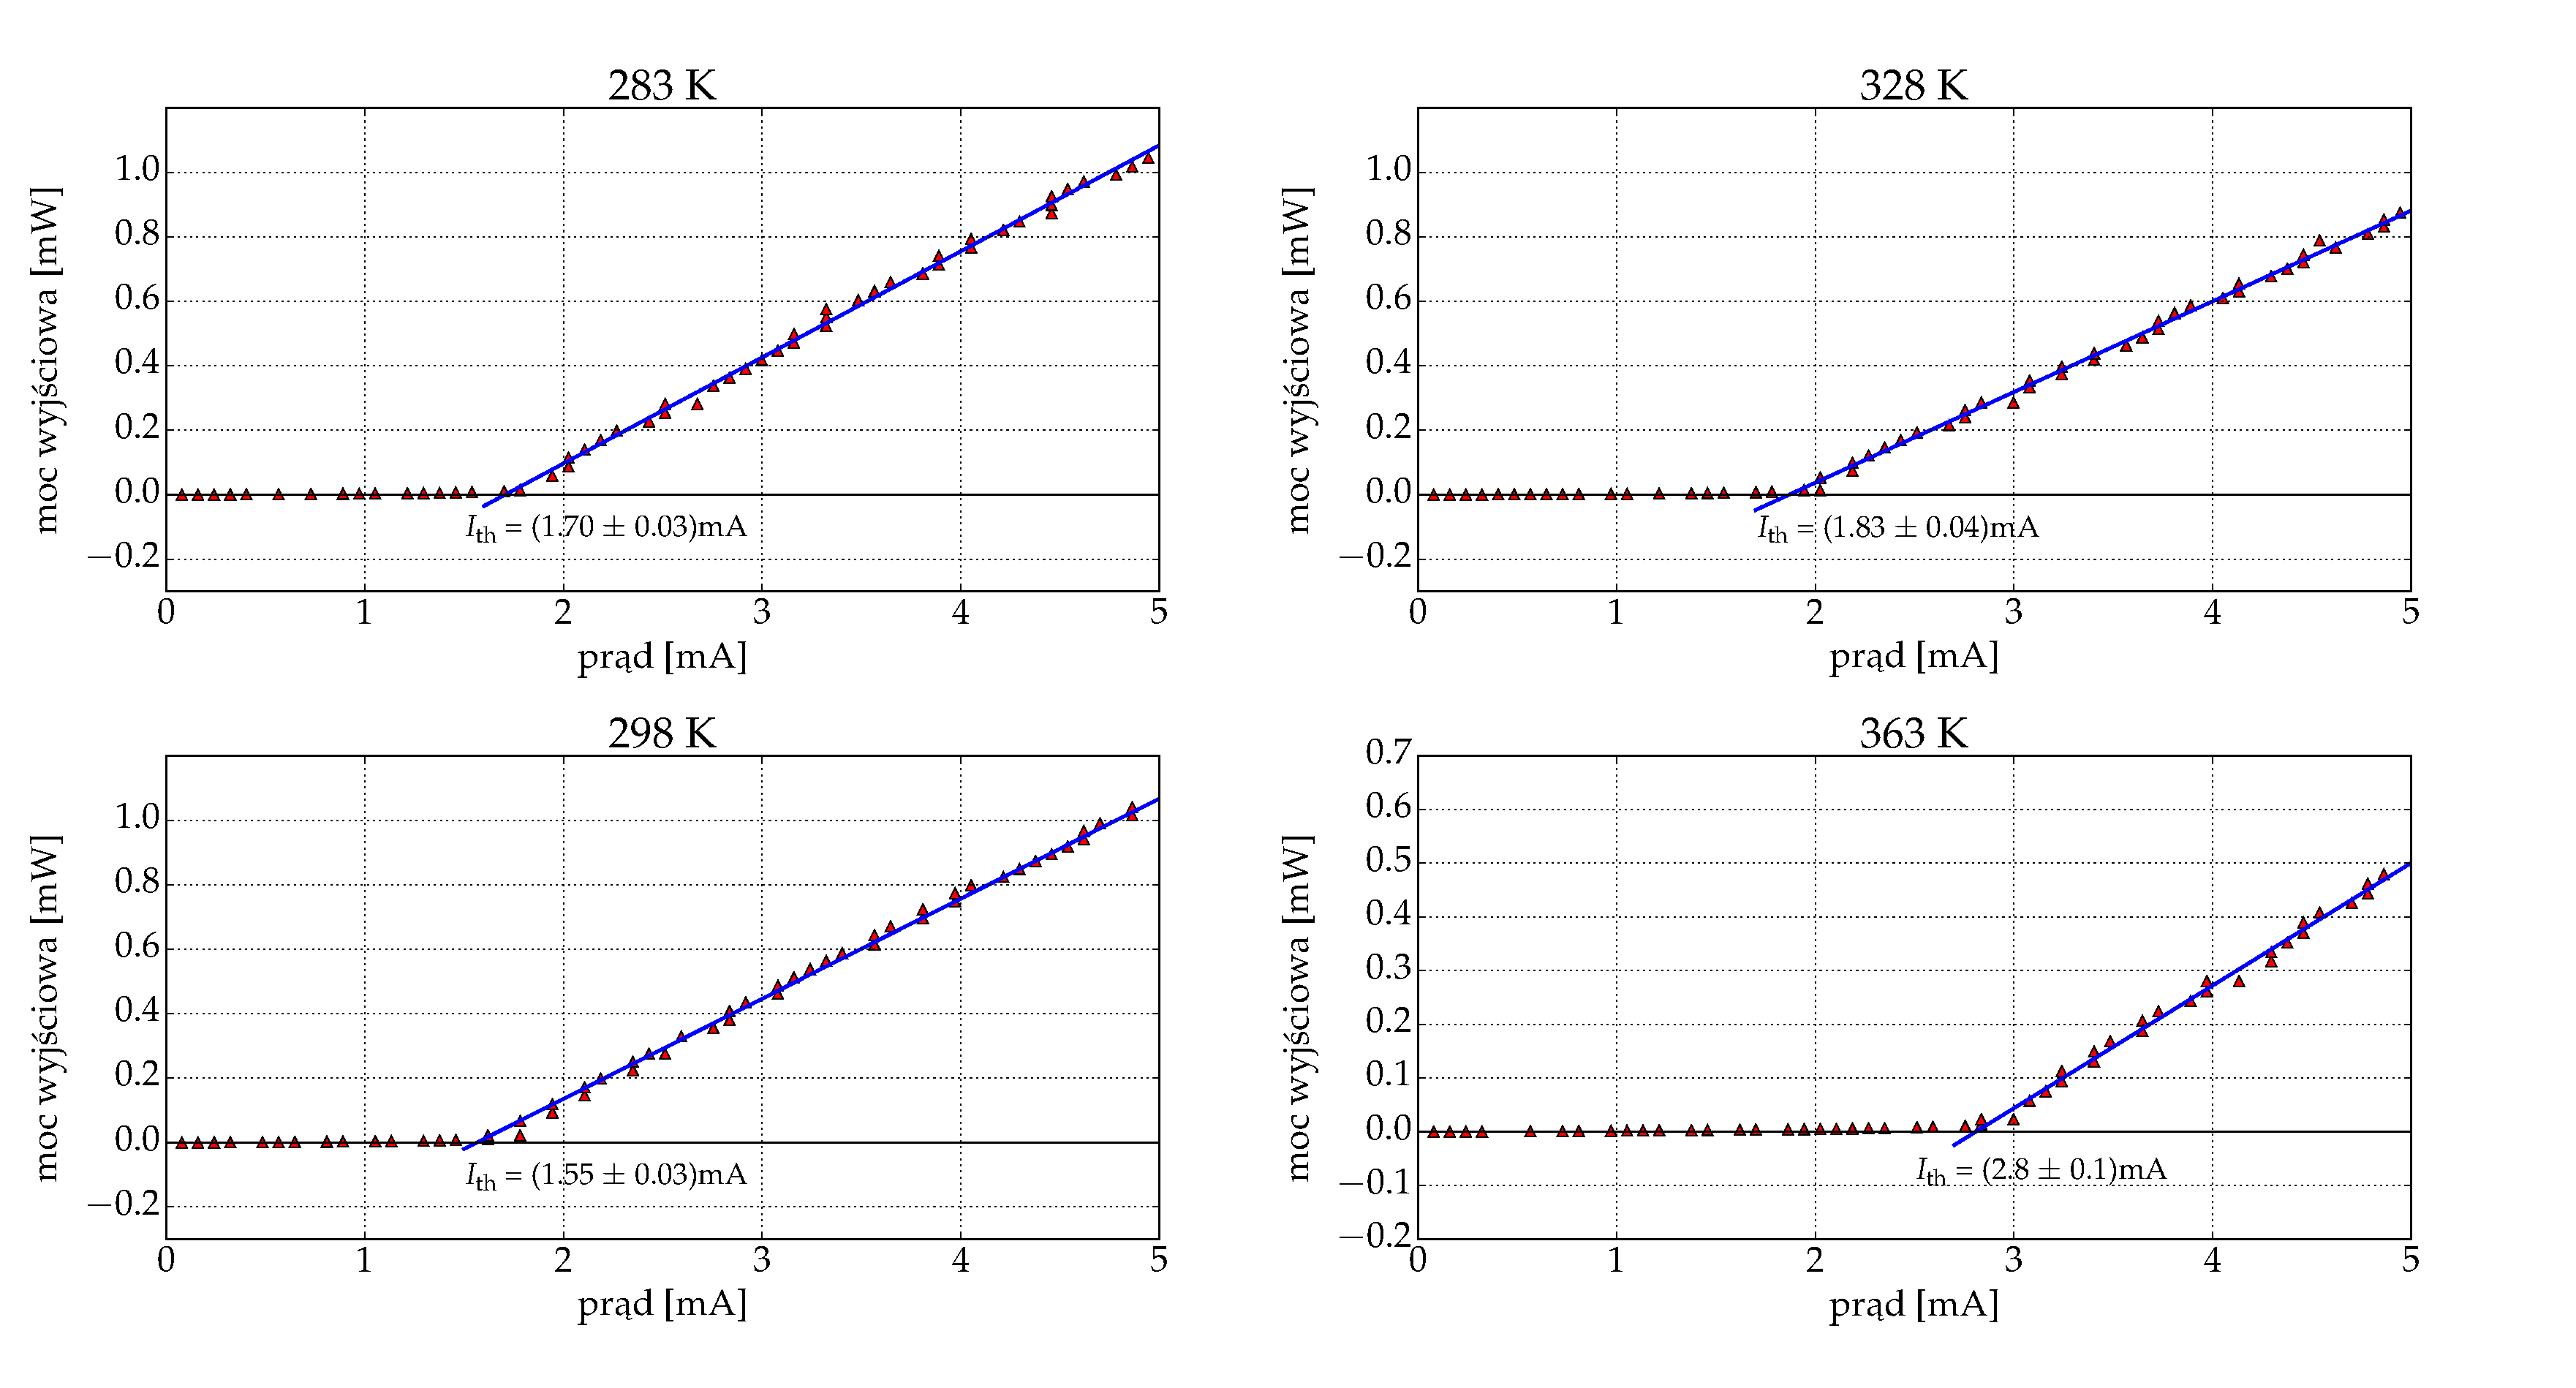
\includegraphics[scale=0.30]{plot_vcsel_850/plot_fit_i_th.eps}
  \caption{Wykres ilustrujący wyznaczanie prądu progowego dla lasera VCSEL 850\,nm.}
  \label{fig:plot_fit_i_th_vcsel850}
\end{figure}
\begin{figure}
\center
  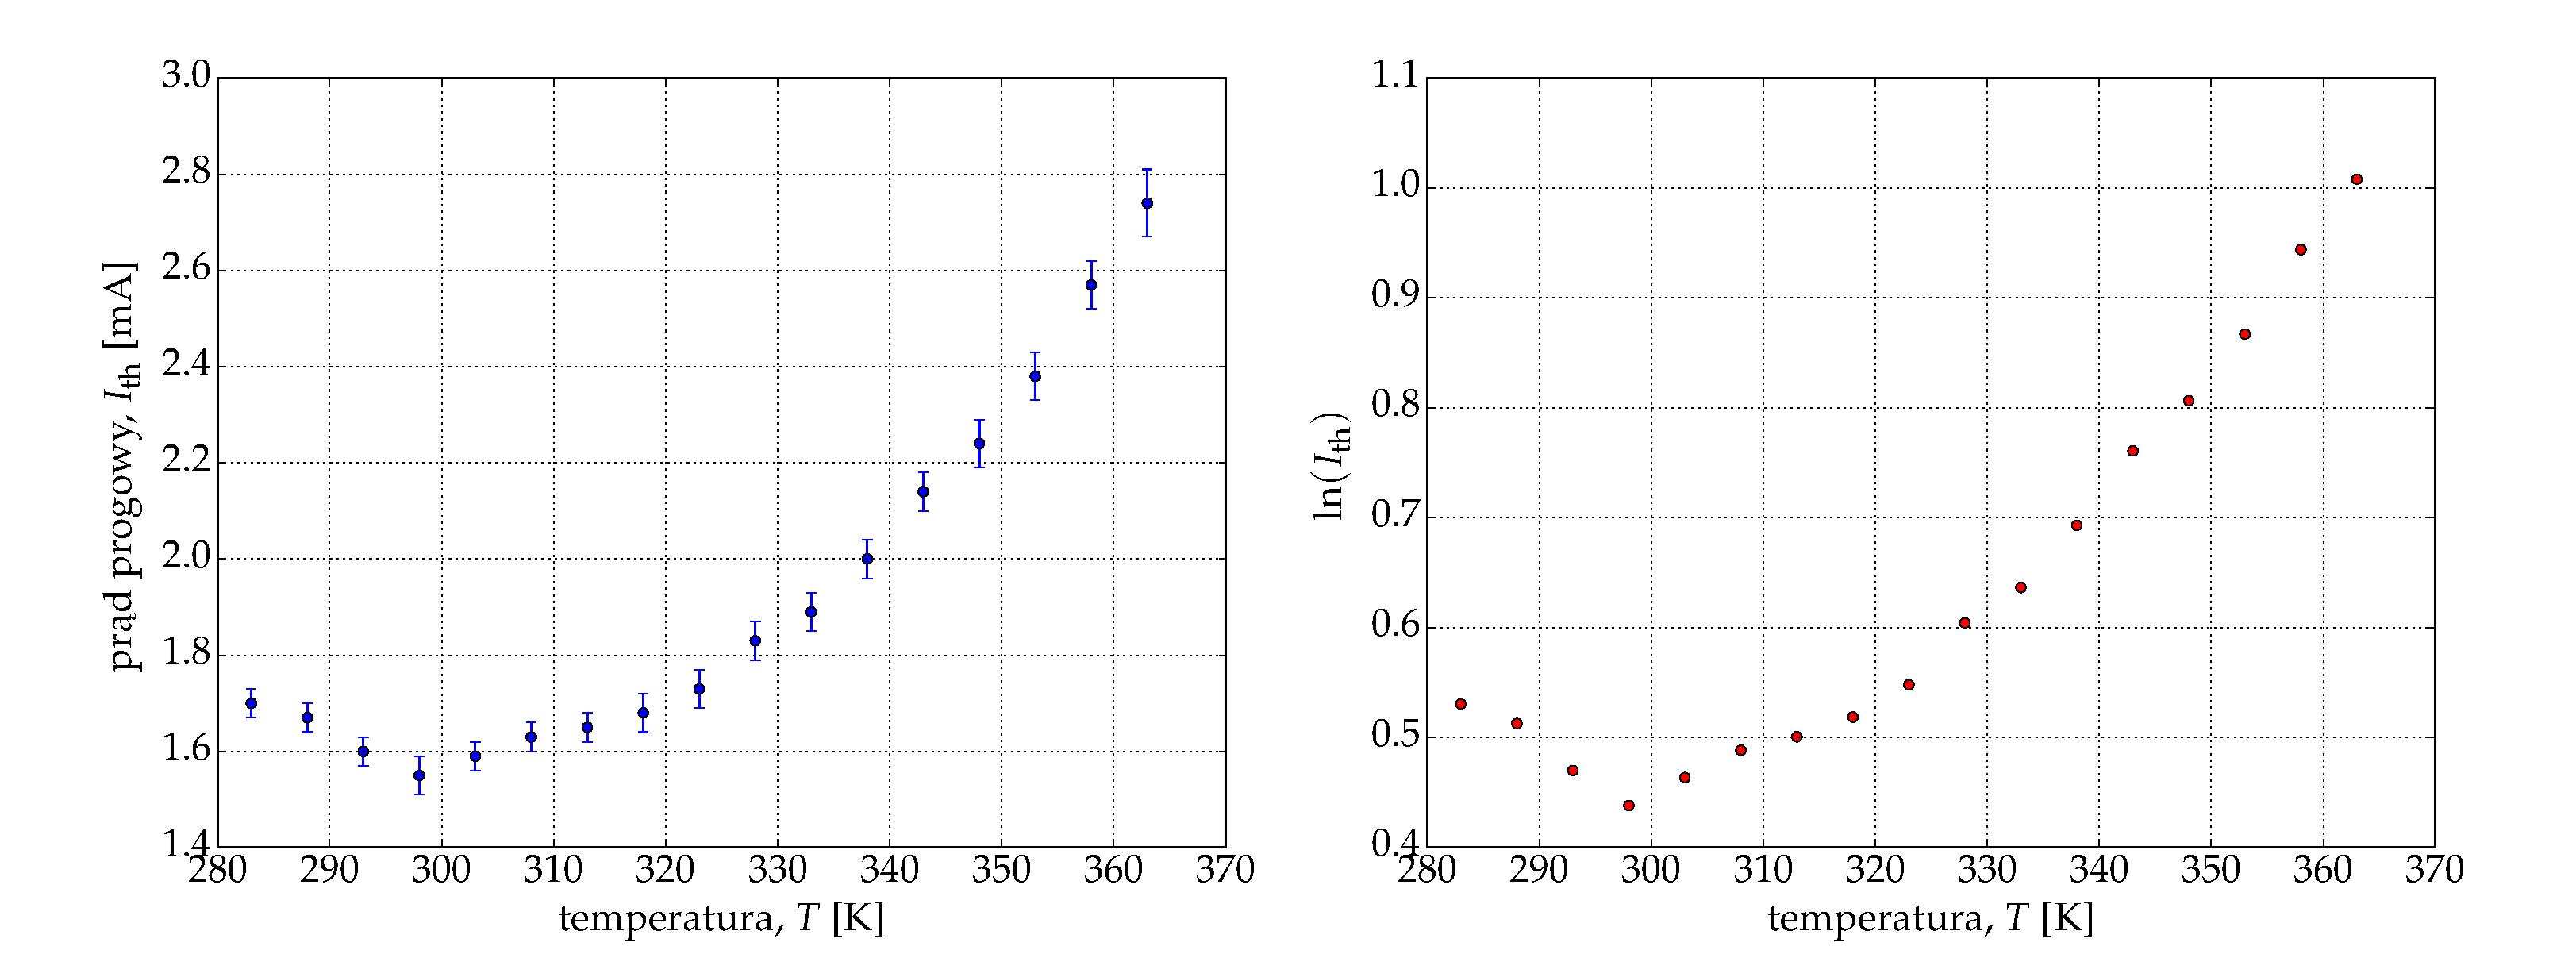
\includegraphics[scale=0.30]{plot_vcsel_850/plot_temp_i_th_log_lin.eps}
  \caption{Wykres prądu progowego od temperatury dla lasera VCSEL 850\,nm.}
  \label{fig:plot_temp_i_th_log_lin_vcsel850}
\end{figure}
%\begin{figure}
%\center
%  \includegraphics[scale=0.30]{plot_vcsel_850/plot_ivl_4.eps}
%  \caption{Sprawność VCSEL 850.}
%  \label{vcsel_850_rys_1}
%\end{figure}
\begin{figure}
\center
  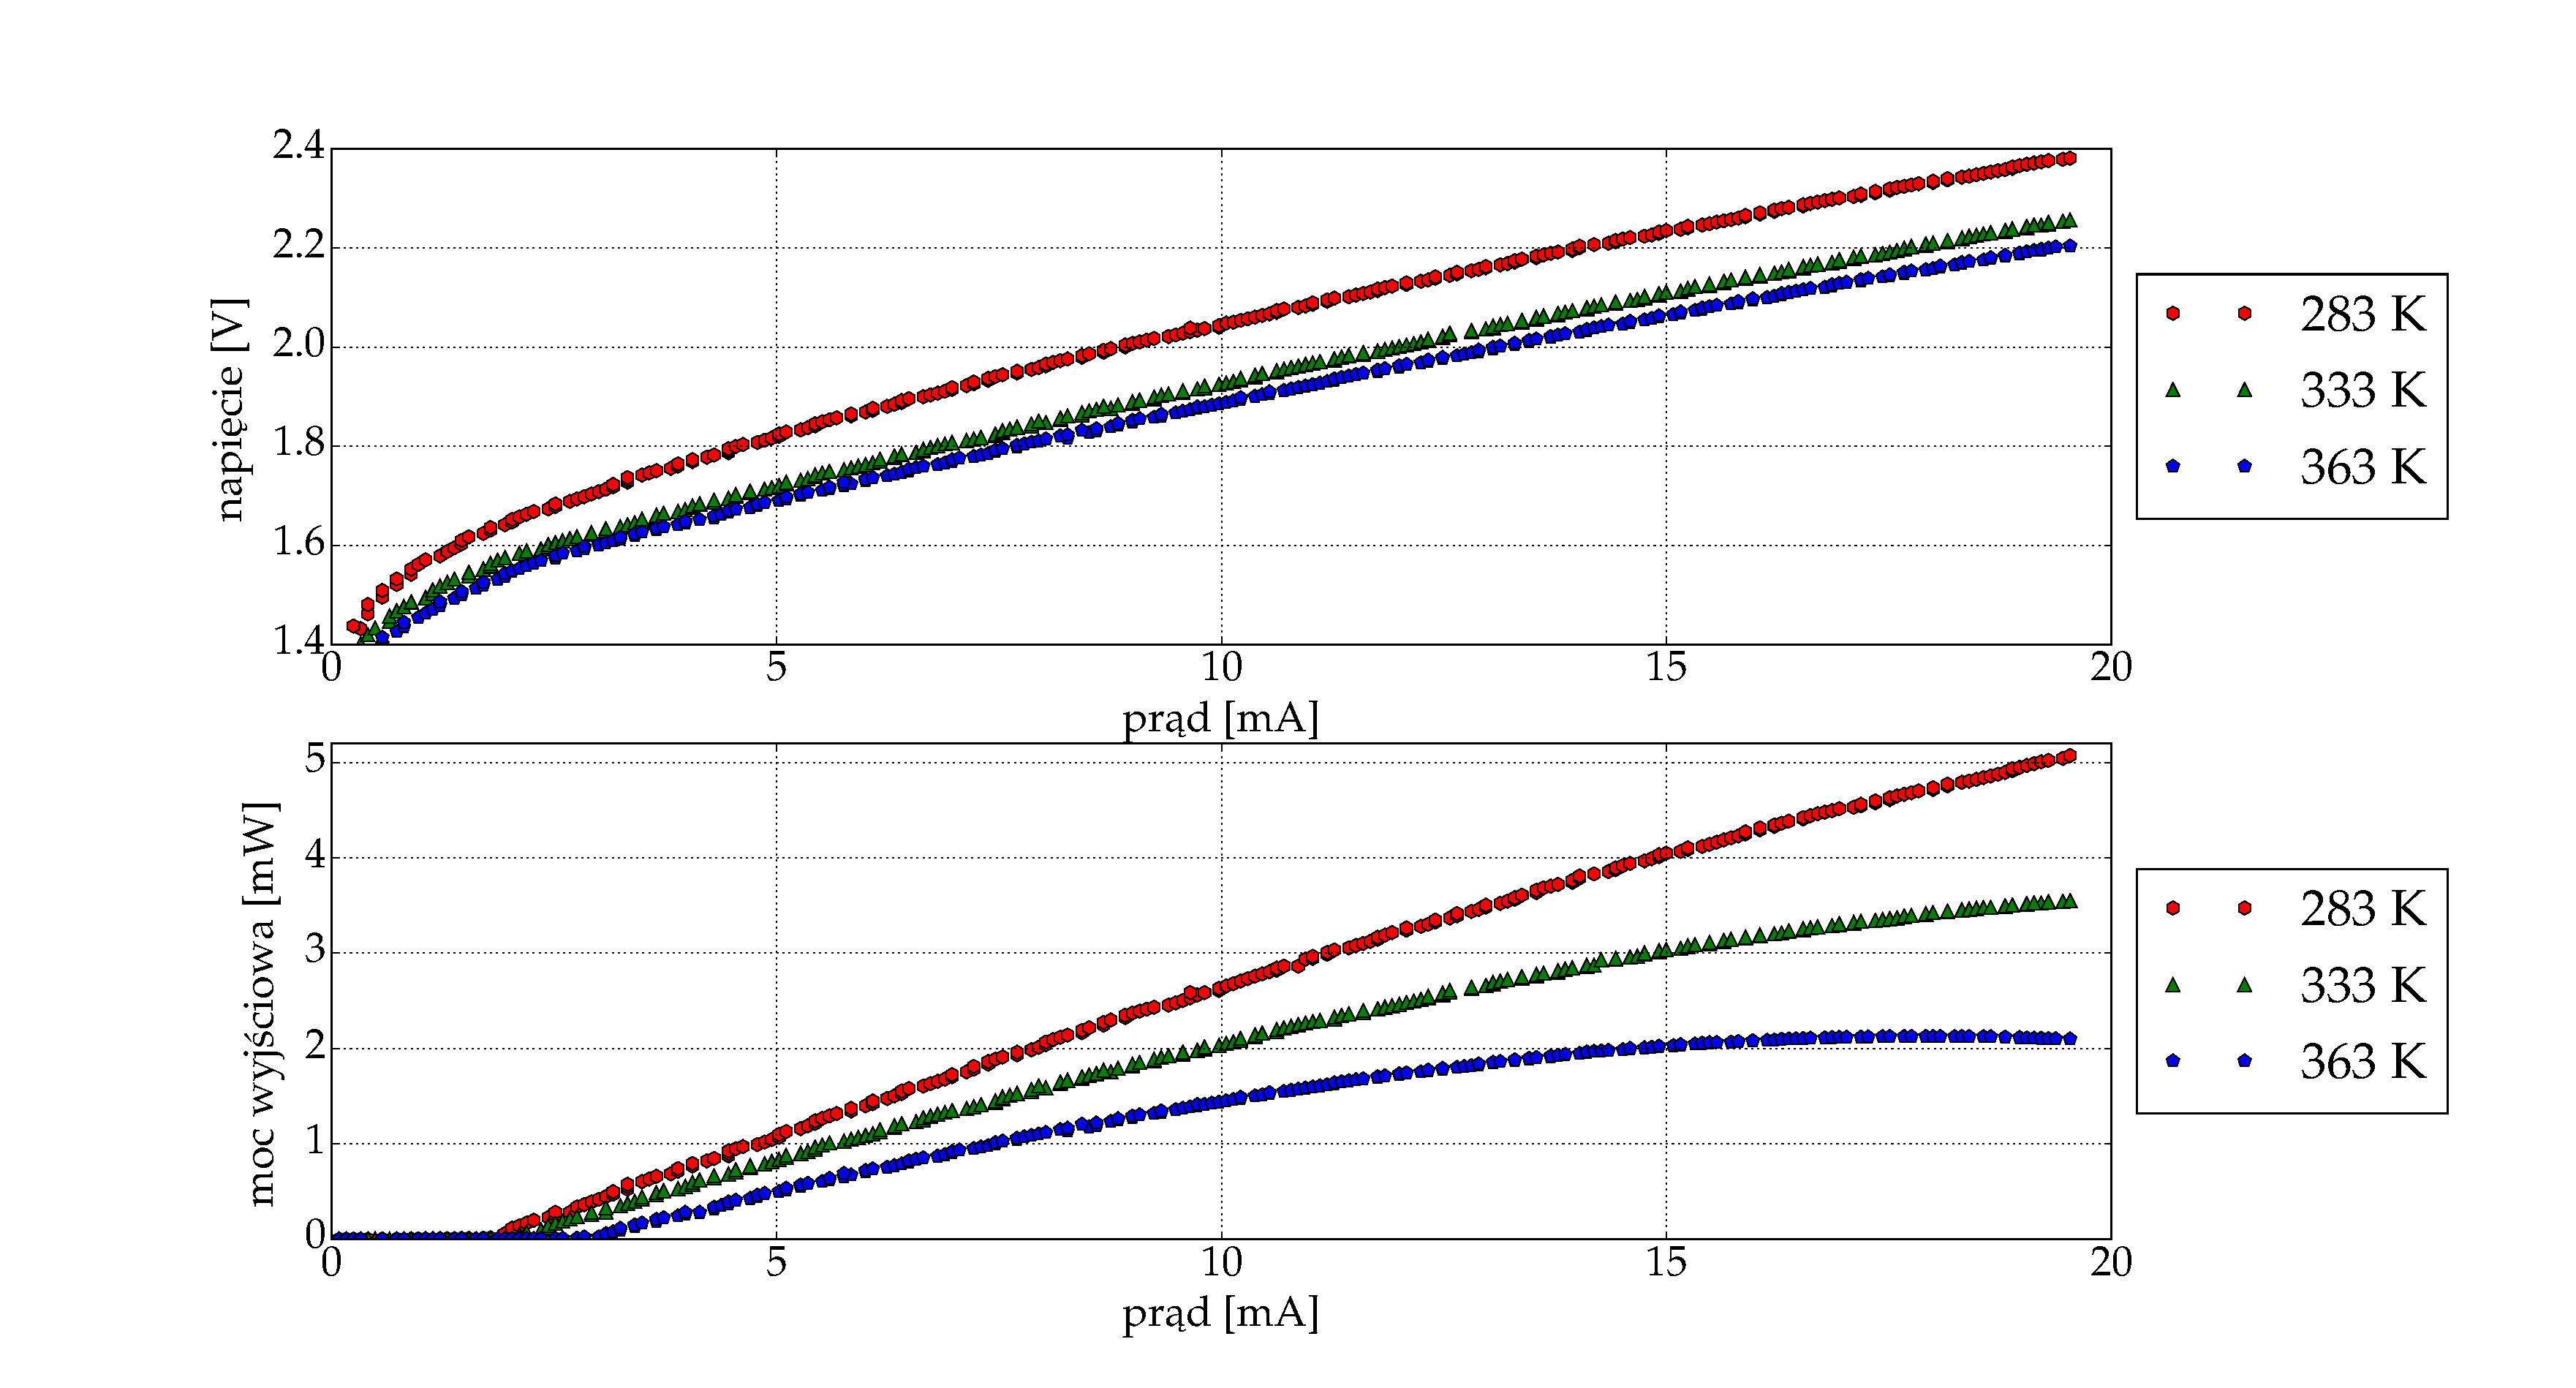
\includegraphics[scale=0.30]{plot_vcsel_850/plot_power_voltage.eps}
  \caption{Wykres napięcia na laserze i mocy wyjściowej w funkcji prądu od temperatury chłodnicy dla lasera VCSEL 850\,nm.}
  \label{fig:plot_power_voltage_vcsel850}
\end{figure}
%\begin{figure}
%\center
%  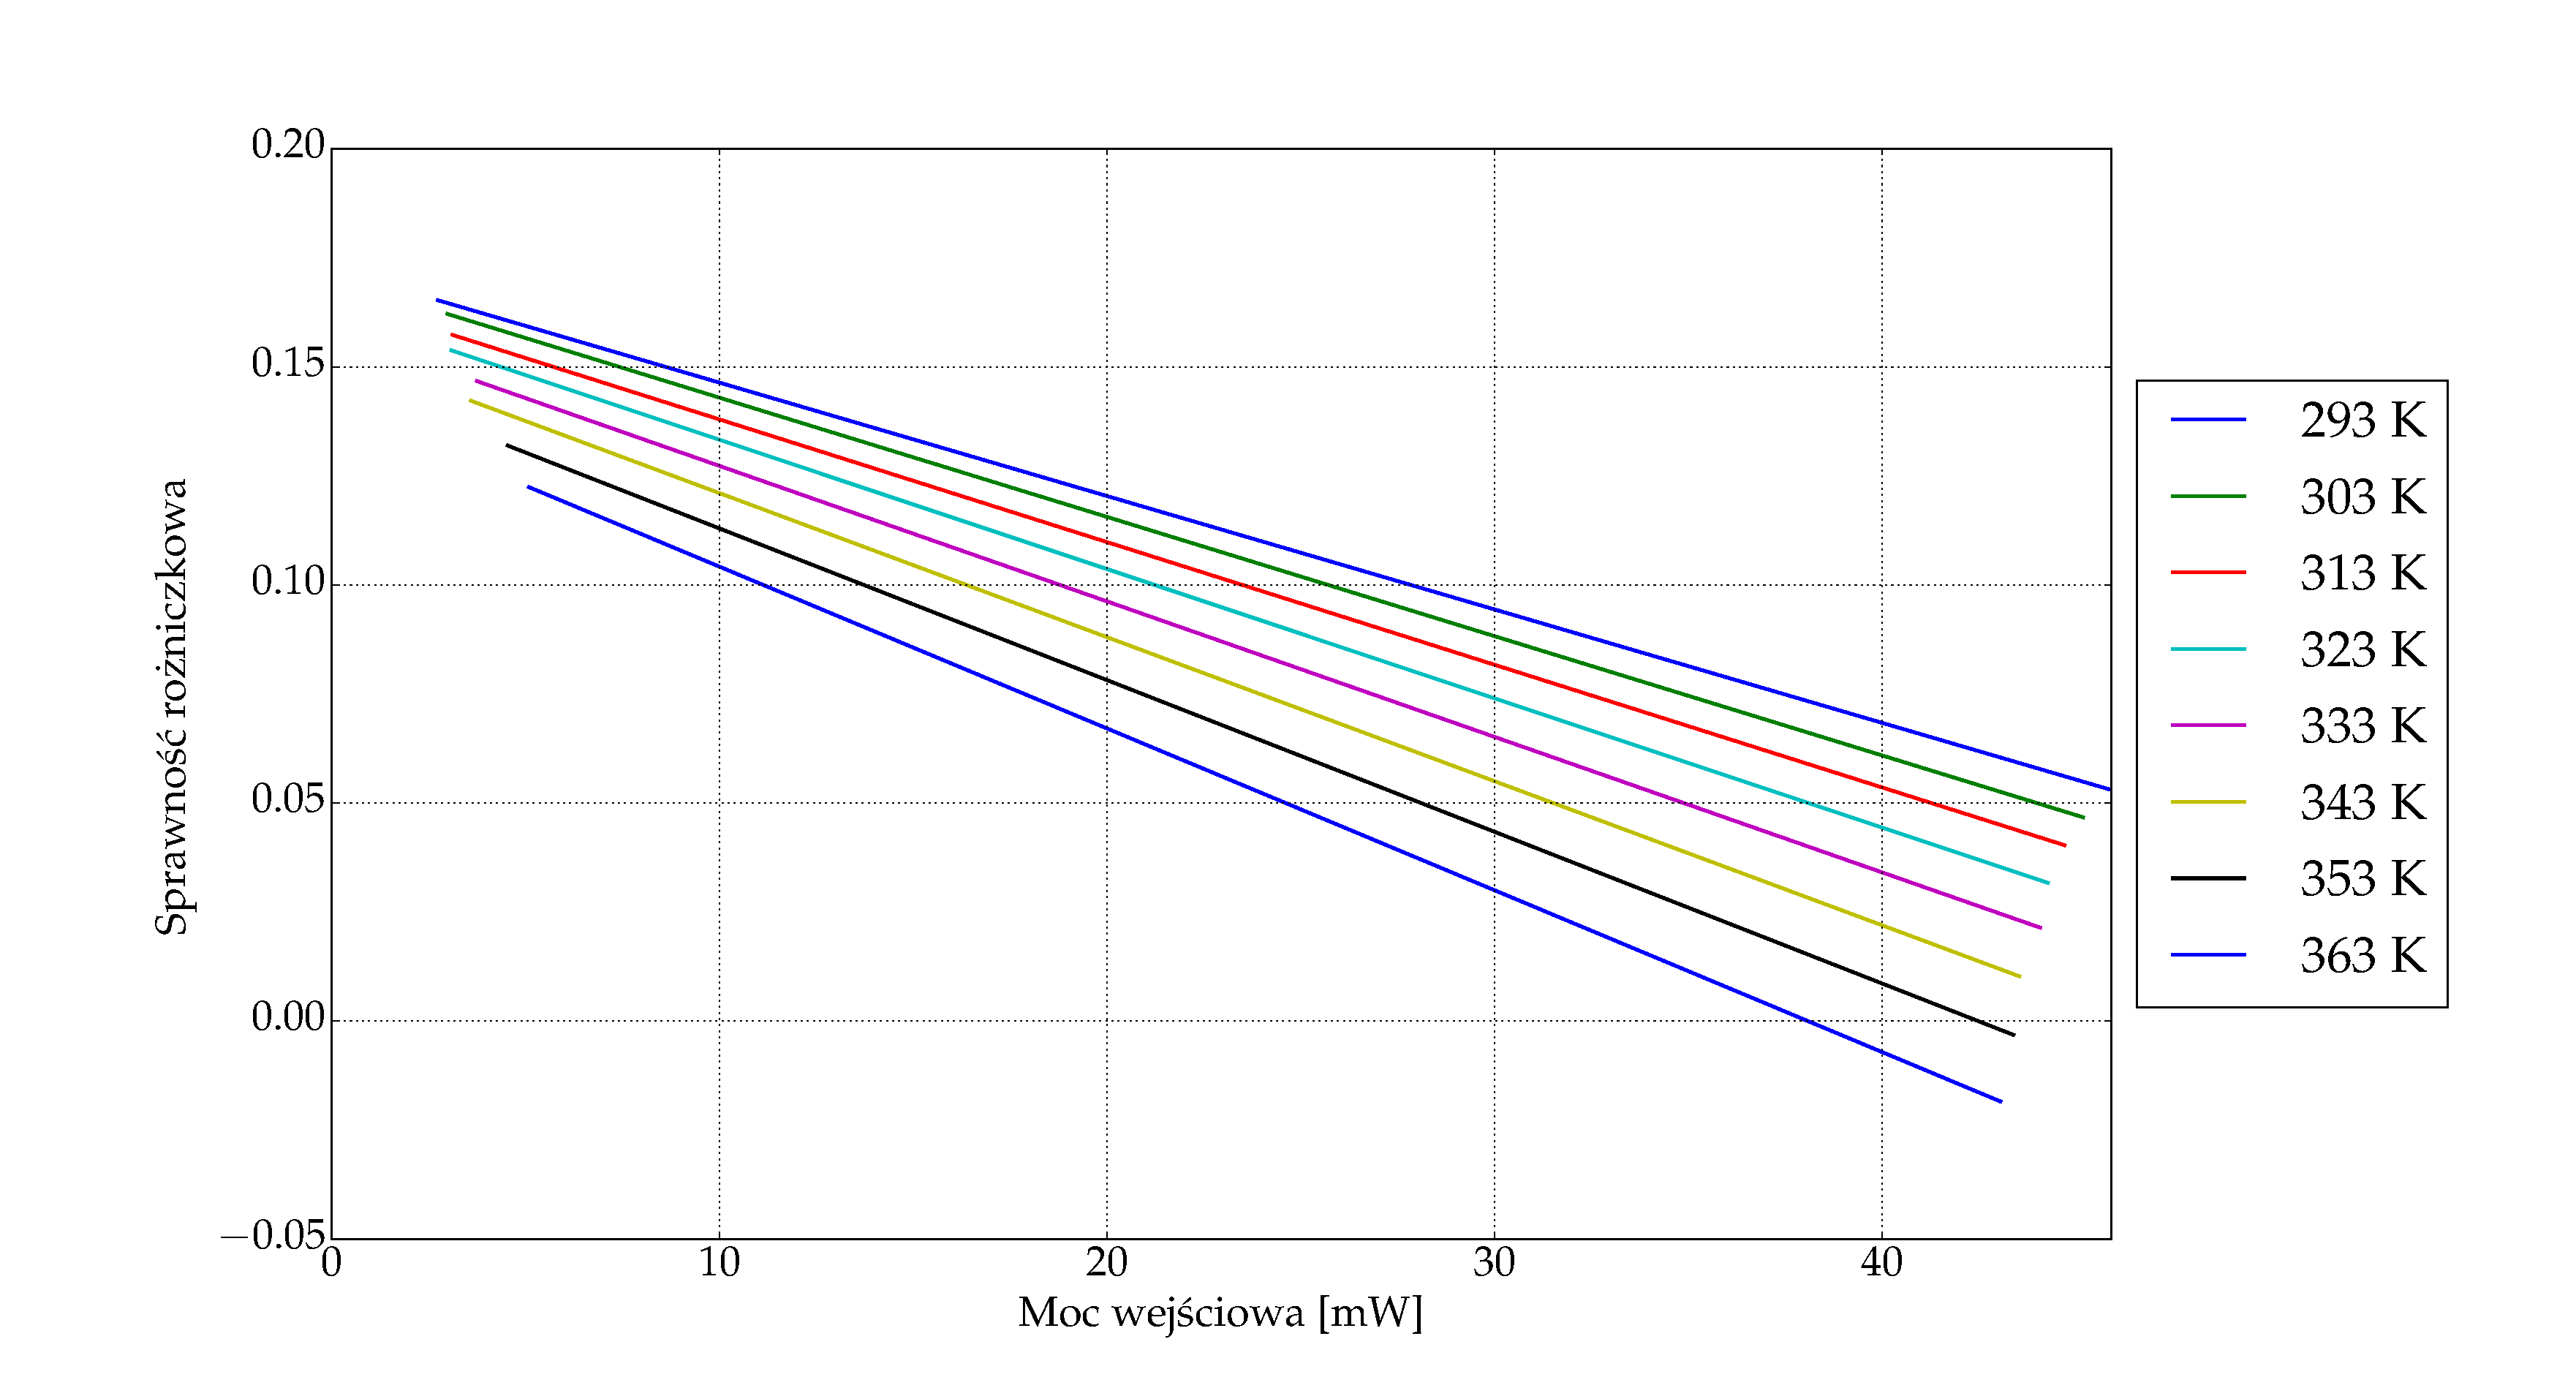
\includegraphics[scale=0.30]{plot_vcsel_850/plot_eff_all_via_power.eps}
%  \caption{Sprawność VCSEL 850 w funkcji mocy wejściowej.}
%  \label{vcsel_850_rys_4}
%\end{figure}
%\begin{figure}
%\center
%  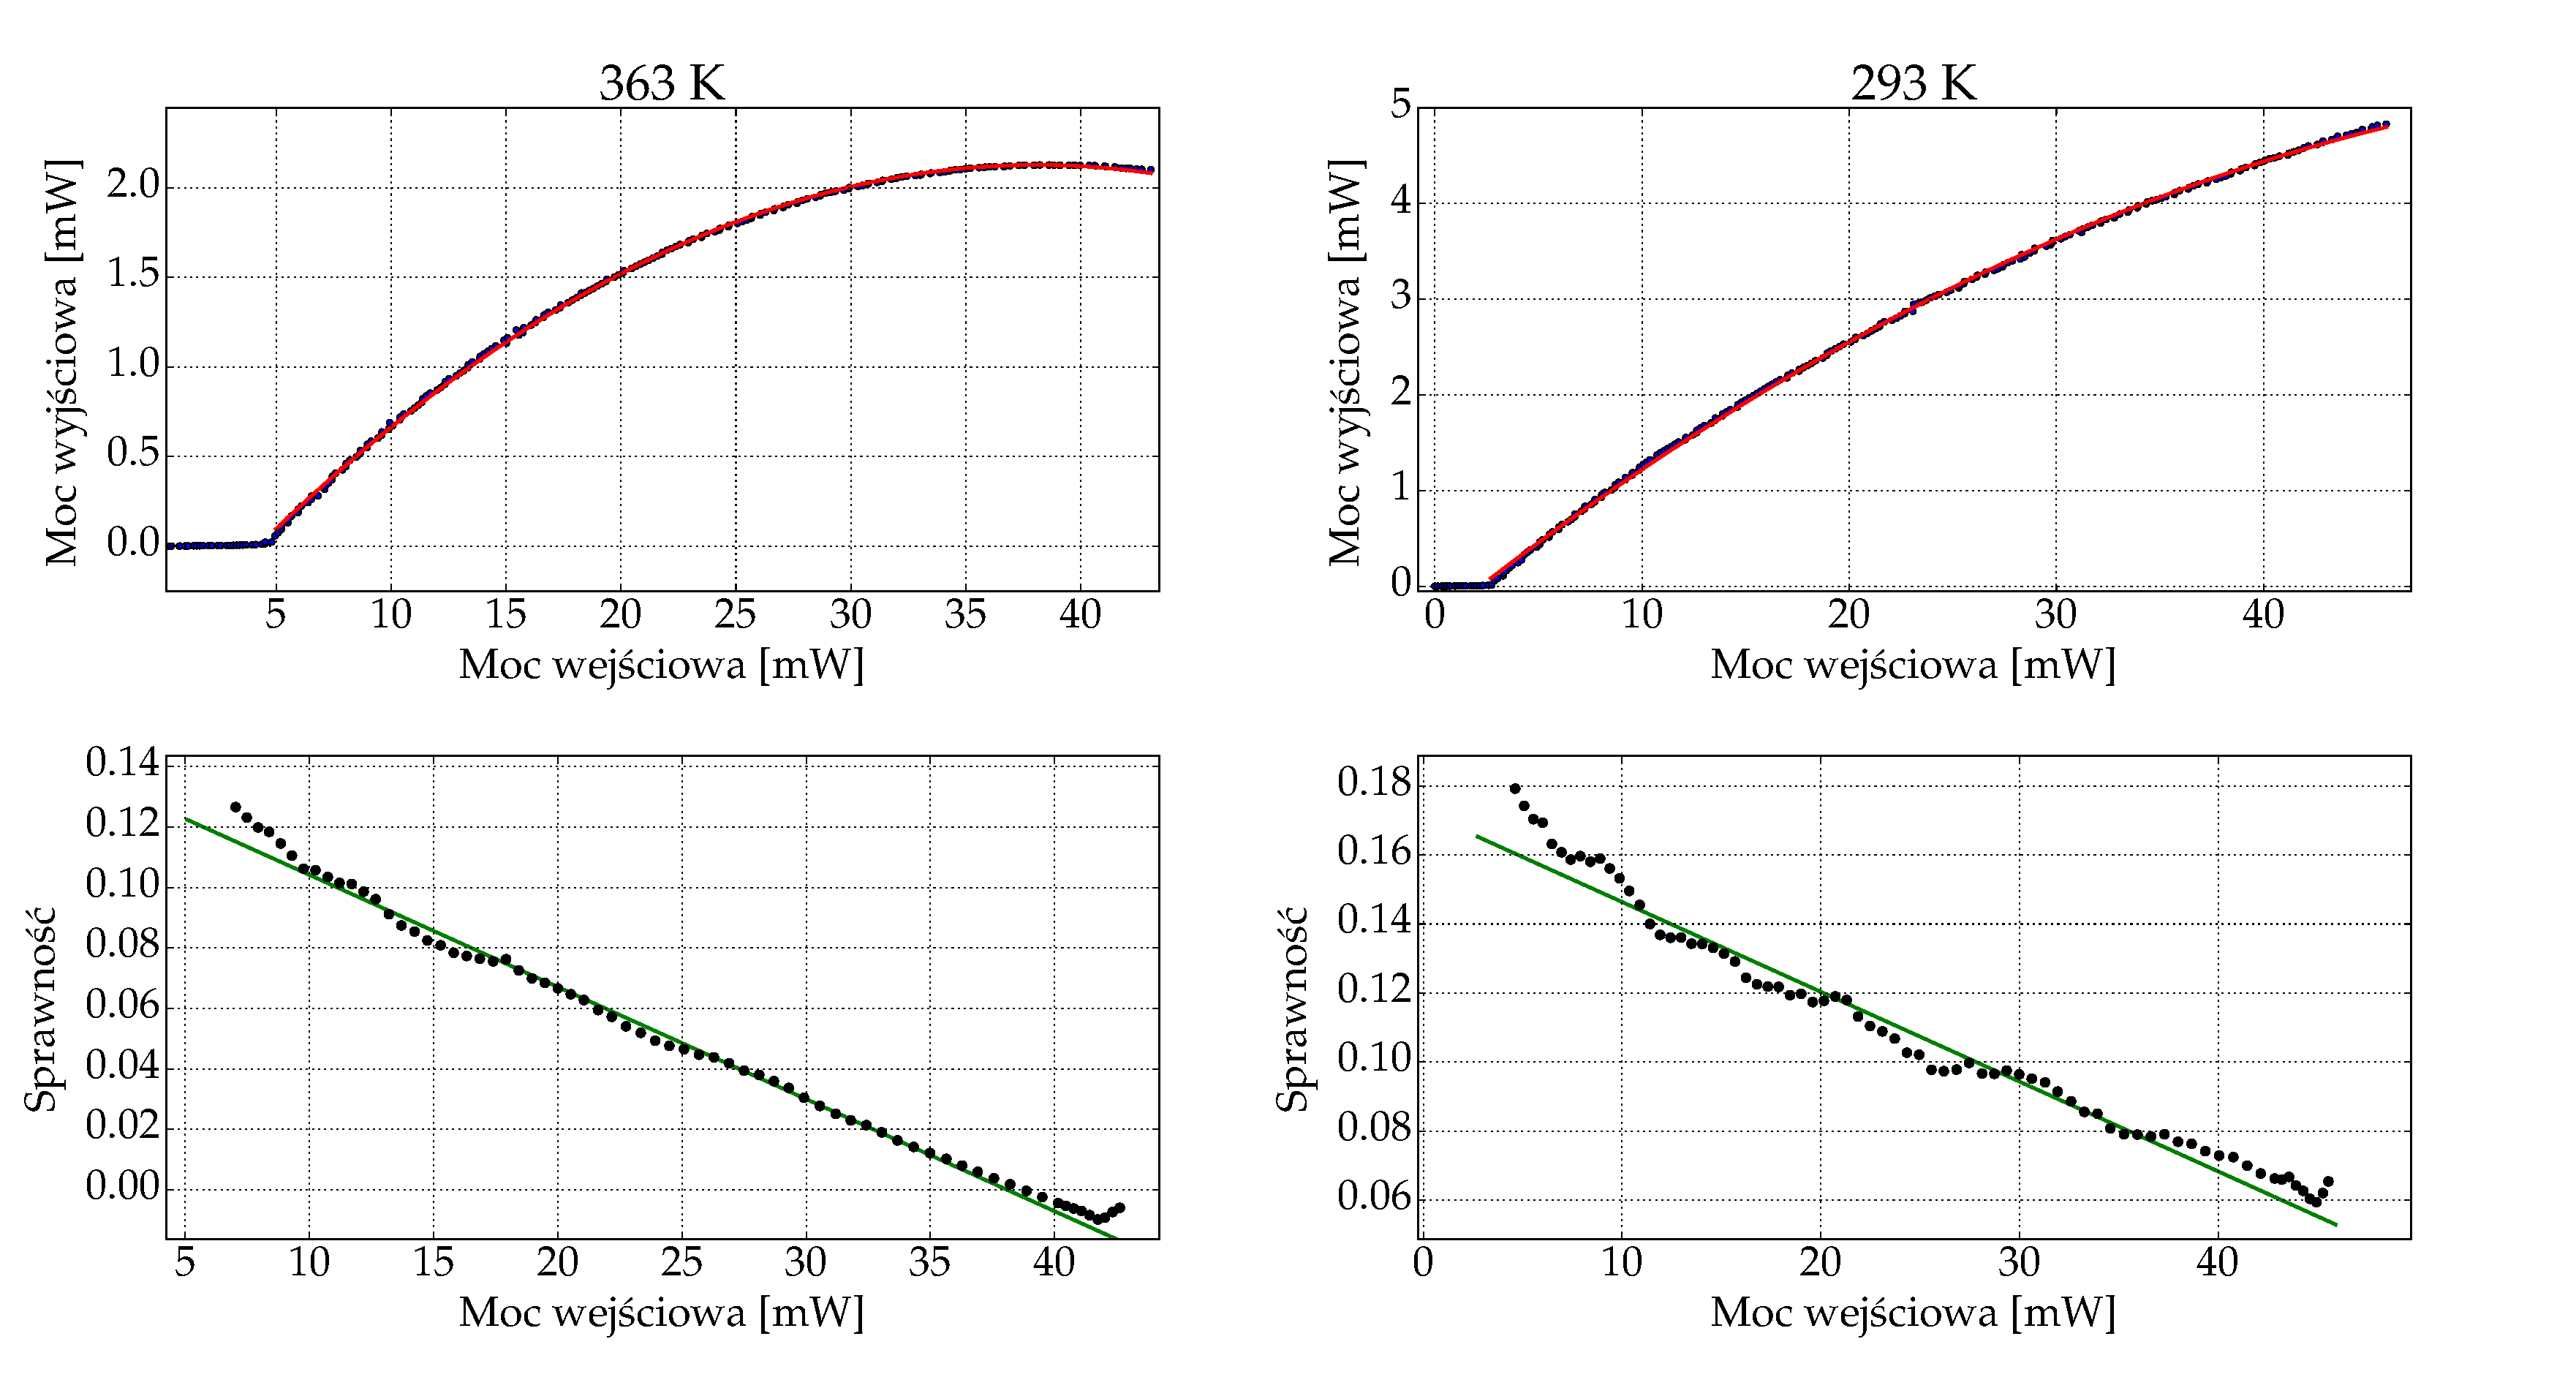
\includegraphics[scale=0.30]{plot_vcsel_850/plot_eff_20_90_via_power.eps}
%  \caption{Sprawność VCSEL 850 dla temperatury 293\,K i 363\,K.}
%  \label{vcsel_850_rys_5}
%\end{figure}
%\begin{figure}
%\center
%  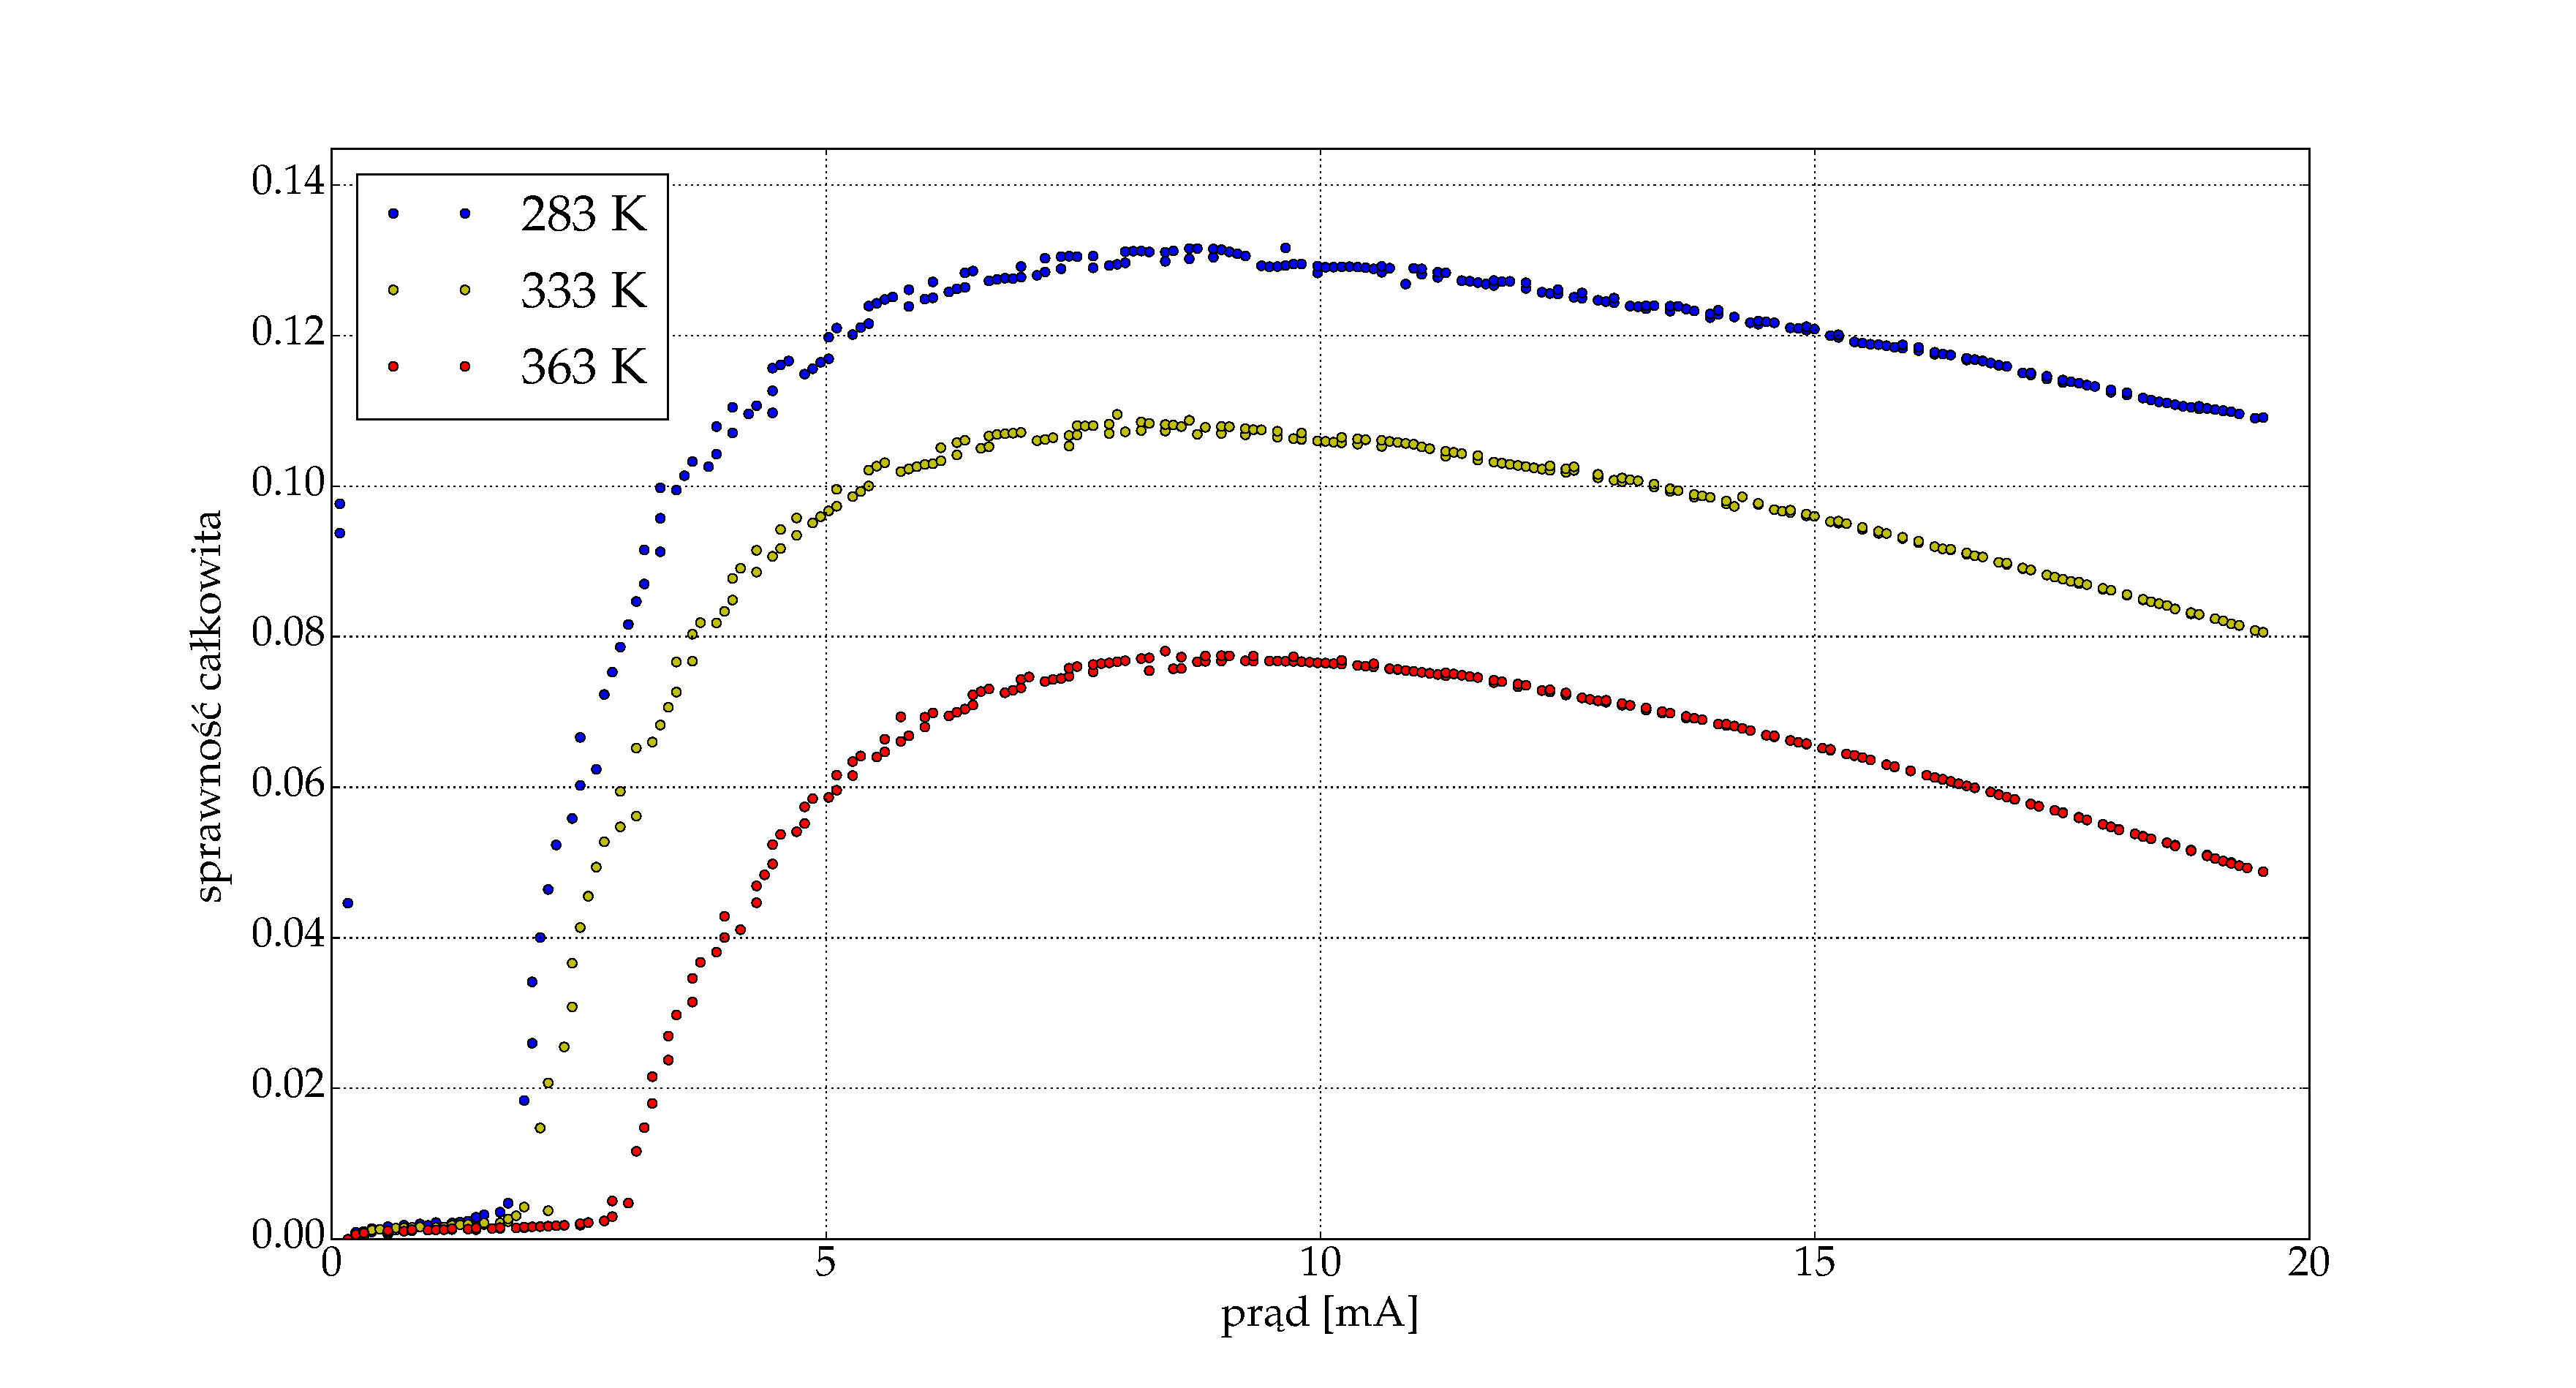
\includegraphics[scale=0.30]{plot_vcsel_850/plot_eff_wall.eps}
%  \caption{Sprawność całkowita dla lasera VCSEL 850\,nm w różnych temperaturach.}
%  \label{vcsel_850_rys_8}
%\end{figure}
\begin{figure}
\center
  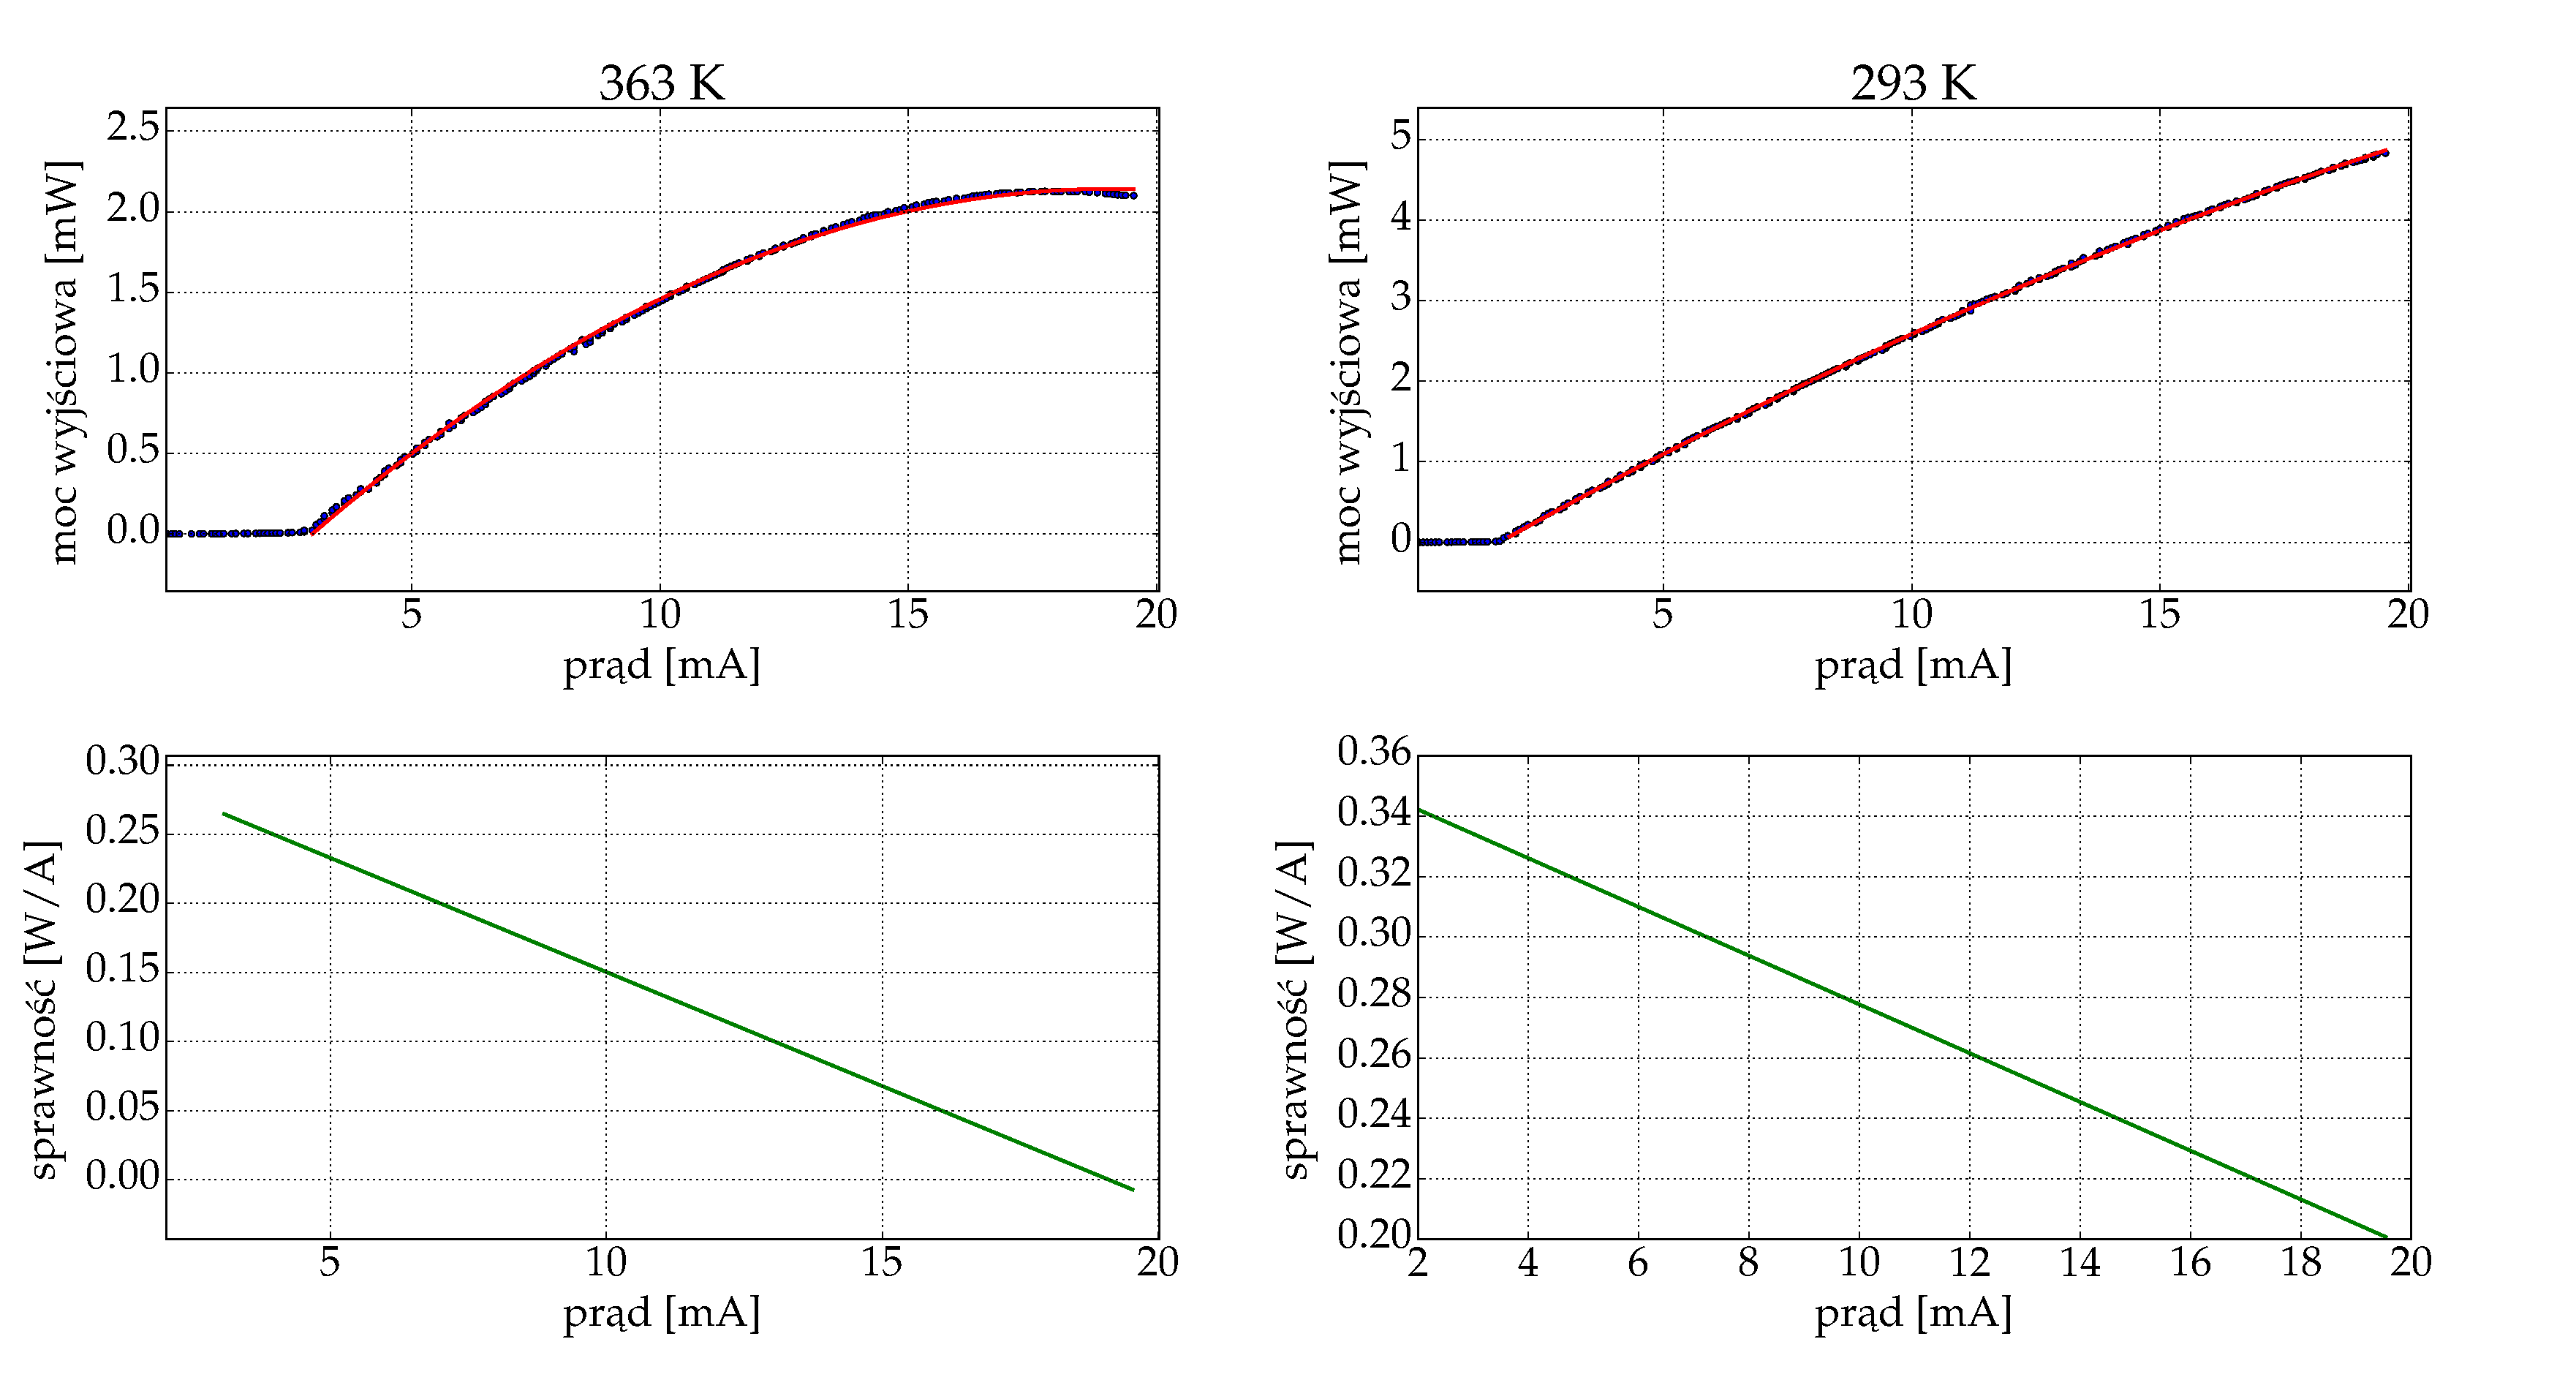
\includegraphics[scale=0.30]{plot_vcsel_850/plot_eff_all_via_current2.eps}
  \caption{Sprawność różniczkowa dla lasera VCSEL 850\,nm w różnych temperaturach.}
  \label{fig:plot_eff_all_via_current2_vcsel850}
\end{figure}
\begin{figure}
\center
  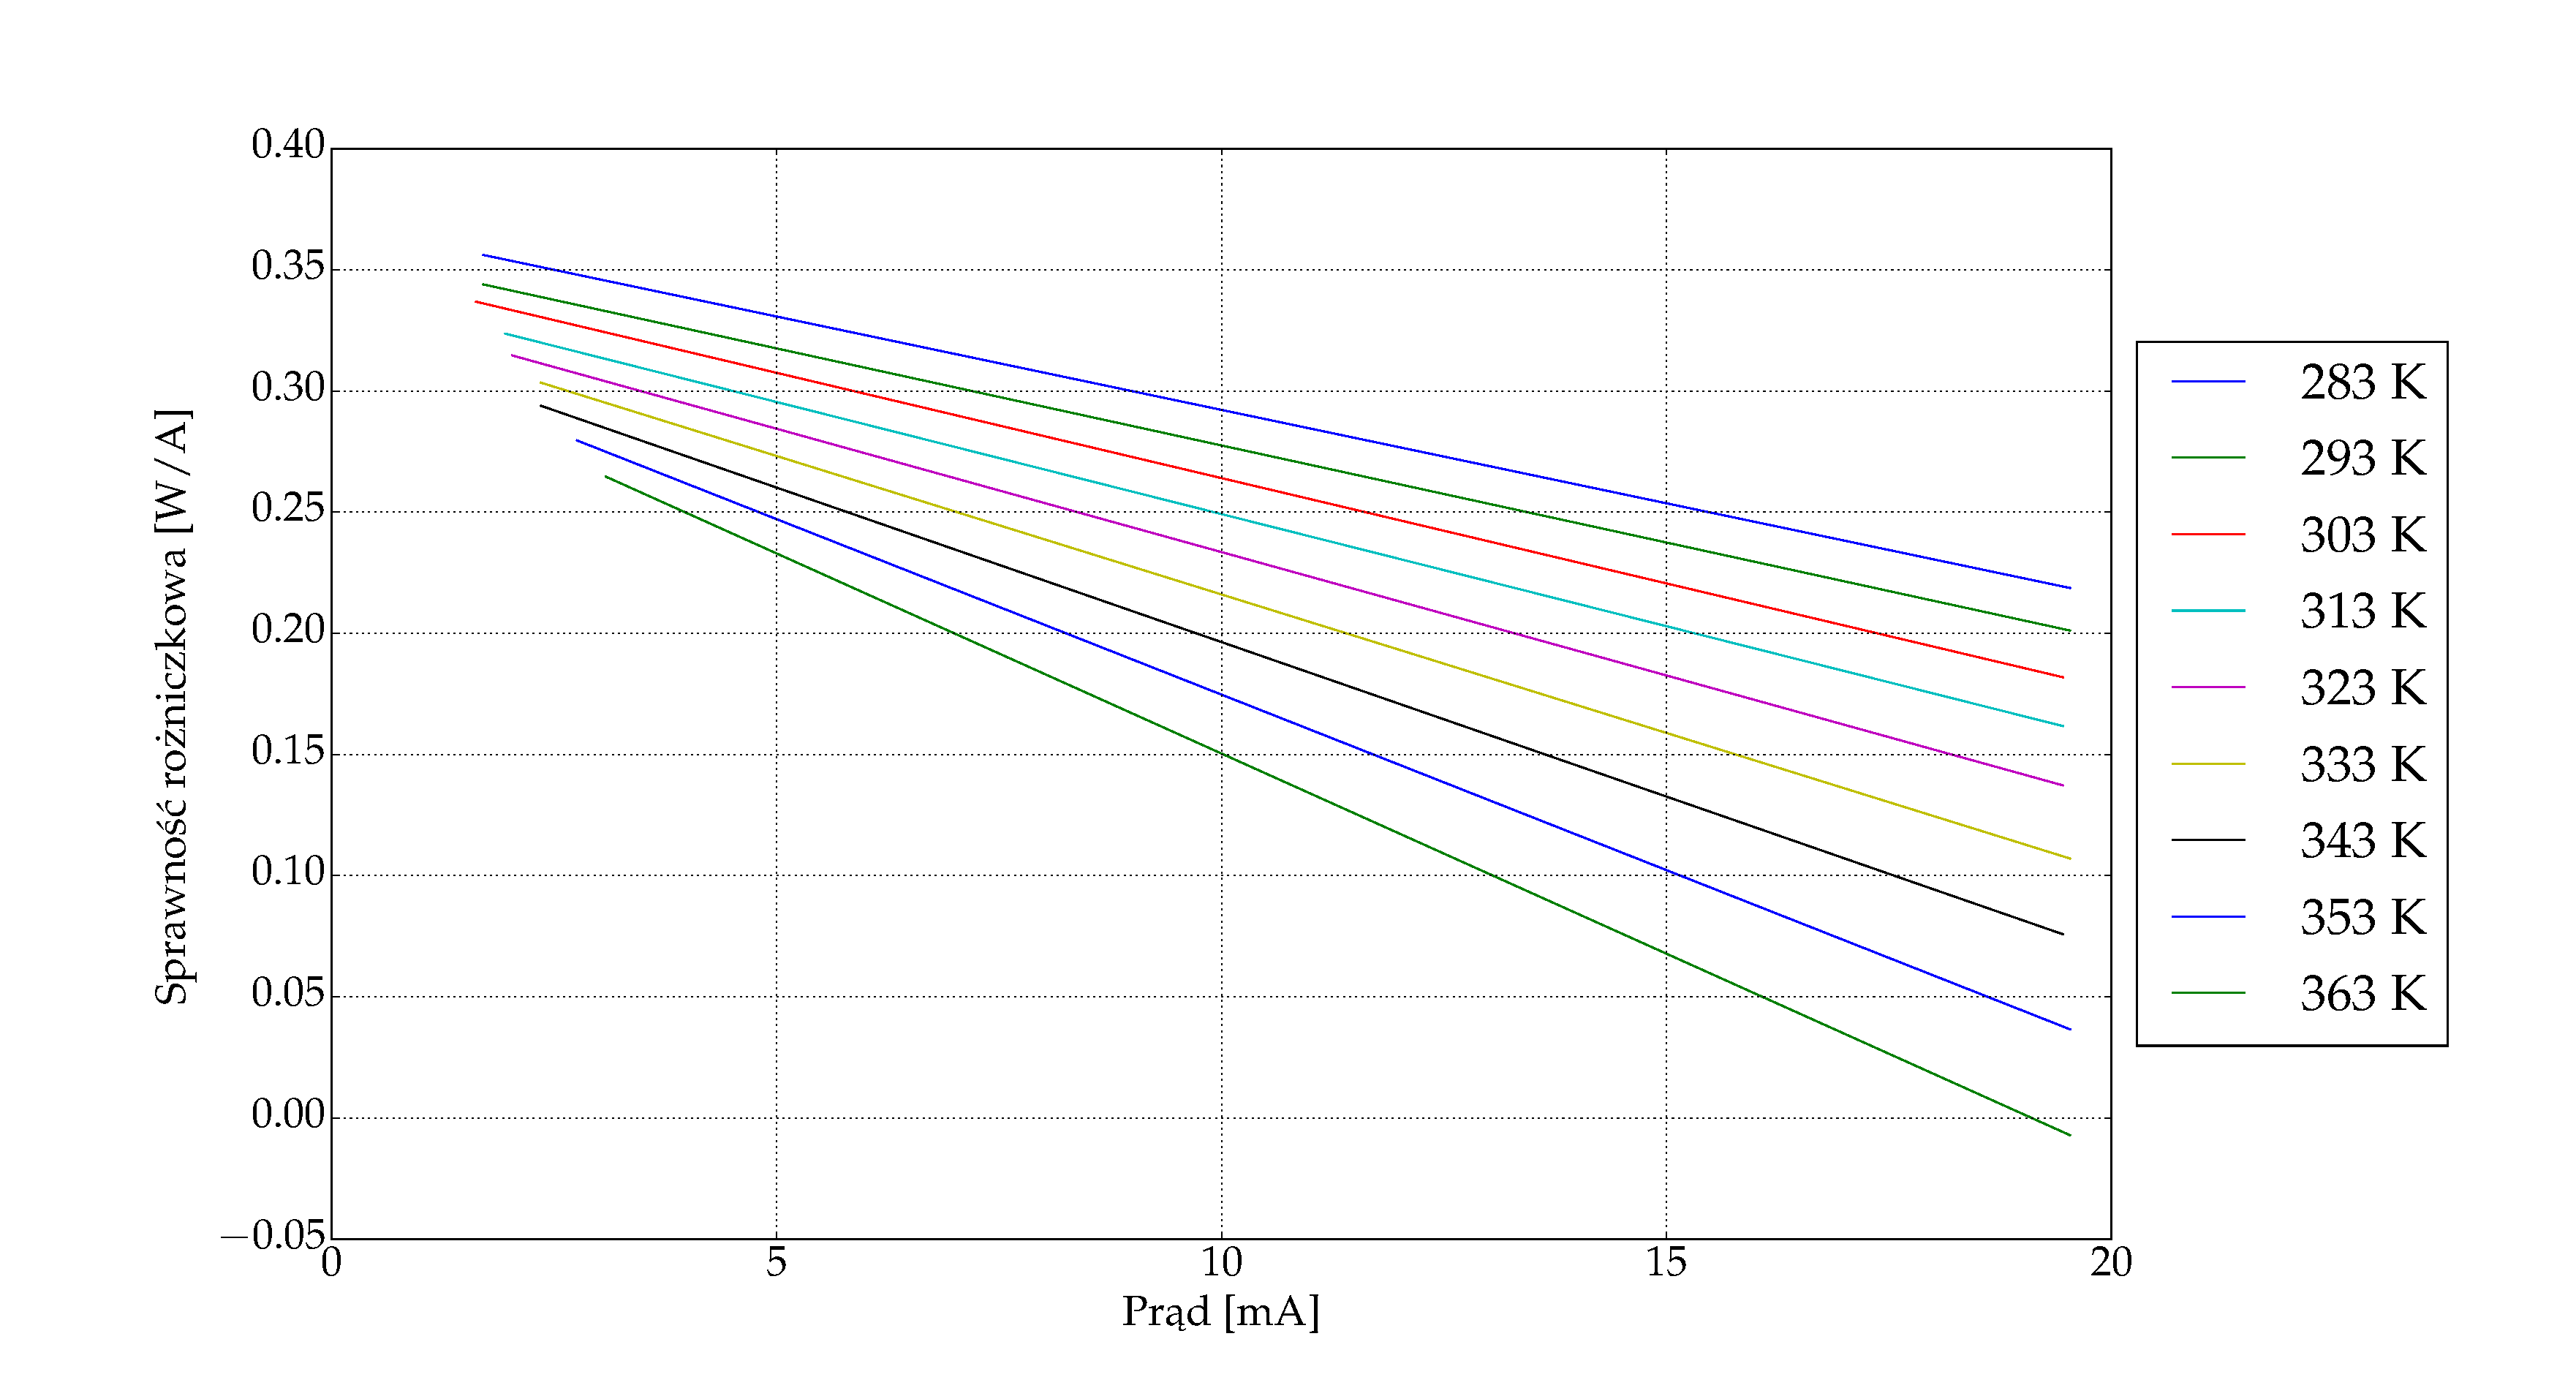
\includegraphics[scale=0.25]{plot_vcsel_850/plot_eff_all_via_current.eps}
  \caption{Sprawność różniczkowa lasera VCSEL 850 w funkcji prądu dla różnych temperatur.}
  \label{fig:plot_eff_all_via_current_vcsel850}
\end{figure}
\newpage
%\section{Omówienie wyników}
%Dzięki analizie sporządzonych wykresów można dojść do następujących konkluzji:
%\begin{itemize}
%\item Analizując wykres napięcia na laserze od prądu wejściowego przedstawiony na rysunku~\ref{vcsel_850_rys_1} oraz~\ref{vcsel_850_rys_2} można zauważyć, że wraz ze wzrostem temperatury na chłodnicy
%maleje opór lasera. Także, wraz z wyższą temperaturą chłodnicy maleje moc wyjściowa lasera.
%\item Wykres na rysunku~\ref{vcsel_850_rys_3} przedstawia sprawność różniczkowa lasera w funkcji prądu wejściowego od temperatury na chłodnicy, jak wynika z wykresu im
%wyższa temperatura tym sprawność lasera mniejsza.
%\item Wykres na rysunku~\ref{vcsel_850_rys_4} przedstawia sprawność różniczkowa lasera w funkcji mocy wejściowej od temperatury na chłodnicy, jak wynika z wykresu im
%wyższa temperatura tym sprawność lasera mniejsza.
%\item Wykres na rysunku~\ref{vcsel_850_rys_5} przedstawia w górnej cześci zależności mocy wyjściowej od mocy wejściowej.
%\item Wykres na rysunku~\ref{vcsel_850_rys_7} pokazuje zależności prądu progowego od temperatury. Jak widzimy przy temperaturach (280-300)\,K
%wraz ze wzrostem temperatury maleje wartość prądu progowego, natomiast dla temperatur $>$ 300\,K im wyższa temperatura to zwiększa się
%wartość prądu progowego.
%\item Wykres na rysunku~\ref{vcsel_850_rys_8} przedstawia sprawnośc całkowitą lasera dla trzech temperatur: 283\,K, 333\,K, 363\,K. Analizując ten wykres
%dochodzę do wniosku, że im wyższa temperatura tym sprawnośc mniejsza.
%\item Wykres na rysunku~\ref{vcsel_850_rys_9} przedstawia sprawności różniczkowe dla dwóch temperatur. W górnej cześci przedstawiona jest charakterystyka
%wyjściowa z dopasawaną funkcją w postaci wielomianu stopnia drugiego. Pochodna tej funkcji jest sprawnością rożniczkową. Na dolnym wykresie przedstawiona
%jest sprawność w postaci prostej będącej pochodną dopasowanej funkcji. Natomiast czarne kropki przedstawiają sprawność powstałą w wyniku obliczenia pochylenia
%10 punktów przefiltrowanych co 3 punkty.
%\end{itemize}

\newpage
\subsection{Laser VCSEL 980\,nm --- omówienie wyników}
Pomiar przeprawadzany był w temperaturach chłodnicy od 283\,K do 363\,K, krokiem co 5\,K. Wartości wyznaczonego prądu progowego
znajdują się w tabeli~\ref{tab:tabela_vcsel850}. Rysunki od ~\ref{fig:plot_fit_i_th4_980} do ~\ref{fig:plot_eff_via_current_all_980} dotyczą lasera
VCSEL 980\,nm.
\begin{itemize}
\item Wykres na rysunku~\ref{fig:plot_fit_i_th4_980} przedstawia sposób wyznaczana wartość prądu progowego. Następnie na podstawie
wyznaczonych wartości w danej temperaturze, sporządziłem wykres prądu progowego w zależności od temperatury
przedstawiony na rysunku~\ref{fig:plot_temp_i_th_log_lin_980}. Jak widzimy wykres ten charakteryzuje się pewnym prądem
minimalnym osiągniętym w temperaturze 288\,K.
\item Analizując wykres napięcia na laserze od prądu wejściowego przedstawiony na rysunku~\ref{fig:plot_i_v_i_l_980}
można zauważyć, że wraz ze wzrostem temperatury na chłodnicy
maleje opór lasera. Także, wraz z wyższą temperaturą chłodnicy maleje moc wyjściowa lasera.
\item Wykres na rysunku~\ref{fig:plot_eff_via_current4_980} przedstawia sprawność różniczkowa lasera w funkcji prądu wejściowego
od temperatury na chłodnicy. W górnej części rysunku pokazana jest zależność mocy wyjściowej od prądu, do której dopasowałem
funkcją kwadratowa dla punktów leżących powyżej wartości prądu progowego. Dopasowana funkcja zbliżona jest do funkcji kwadratowej,
przez co zmiany sprawności wraz z wzrostem prądu jest dosyć duża.
\item Wykres na rysunku~\ref{fig:plot_eff_via_current_all_980} przedstawia jak zmienia się sprawność lasera od temperatury chłodnicy.
Funkcje, które przedstawiają sprawność zostały wyznaczone analogicznie jak te przedstawione na rysunku~\ref{fig:plot_eff_via_current4_980}.
Analizując ten wykres, dochodzę do wniosku, że wraz z wyższą temperaturą sprawność lasera maleje.
\end{itemize}
\begin{table}
\begin{center}
\caption{ Wyznaczone wartośc prądu progowego $I_{\mathrm{th}}$ w różnych temperaturach $T$ dla lasera VCSEL 980\,nm.}
\begin{tabular}{ | C{1.5cm}|  C{3.0cm} | C{1.5cm} | C{3.0cm}| C{1.5cm} | C{3.0cm}|}
\hline
$T$ [K] &   $I_{\mathrm{th}}$ [mA]  &  $T$ [K] &   $I_{\mathrm{th}}$ [mA]  &  $T$ [K] &   $I_{\mathrm{th}}$ [mA] 	\\ \hline
283      &   1.0 $\pm$ 0.04  & 288      &   0.94 $\pm$ 0.03       & 293		 &   0.98 $\pm$ 0.03  \\ \hline
298		 &   1.05 $\pm$ 0.04  & 303		 &   1.1 $\pm$ 0.03  & 308		 &   1.18 $\pm$ 0.03  \\ \hline
313		 &   1.23 $\pm$ 0.03  & 318		 &   1.25 $\pm$ 0.03  & 323		 &   1.36 $\pm$ 0.04  \\ \hline
328		 &   1.47 $\pm$ 0.03  & 333		 &   1.59 $\pm$ 0.04    & 338		 &   1.63 $\pm$ 0.04  \\ \hline
343		 &   1.76 $\pm$ 0.04    & 348		 &   1.86 $\pm$ 0.06    & 353		 &   2.07 $\pm$ 0.05  \\ \hline
358      &   2.25 $\pm$ 0.06  & 363 & 2.48 $\pm$ 0.06 \\ \cline{1-4}
\end{tabular}
\end{center}
\end{table}
\begin{figure}
\center
  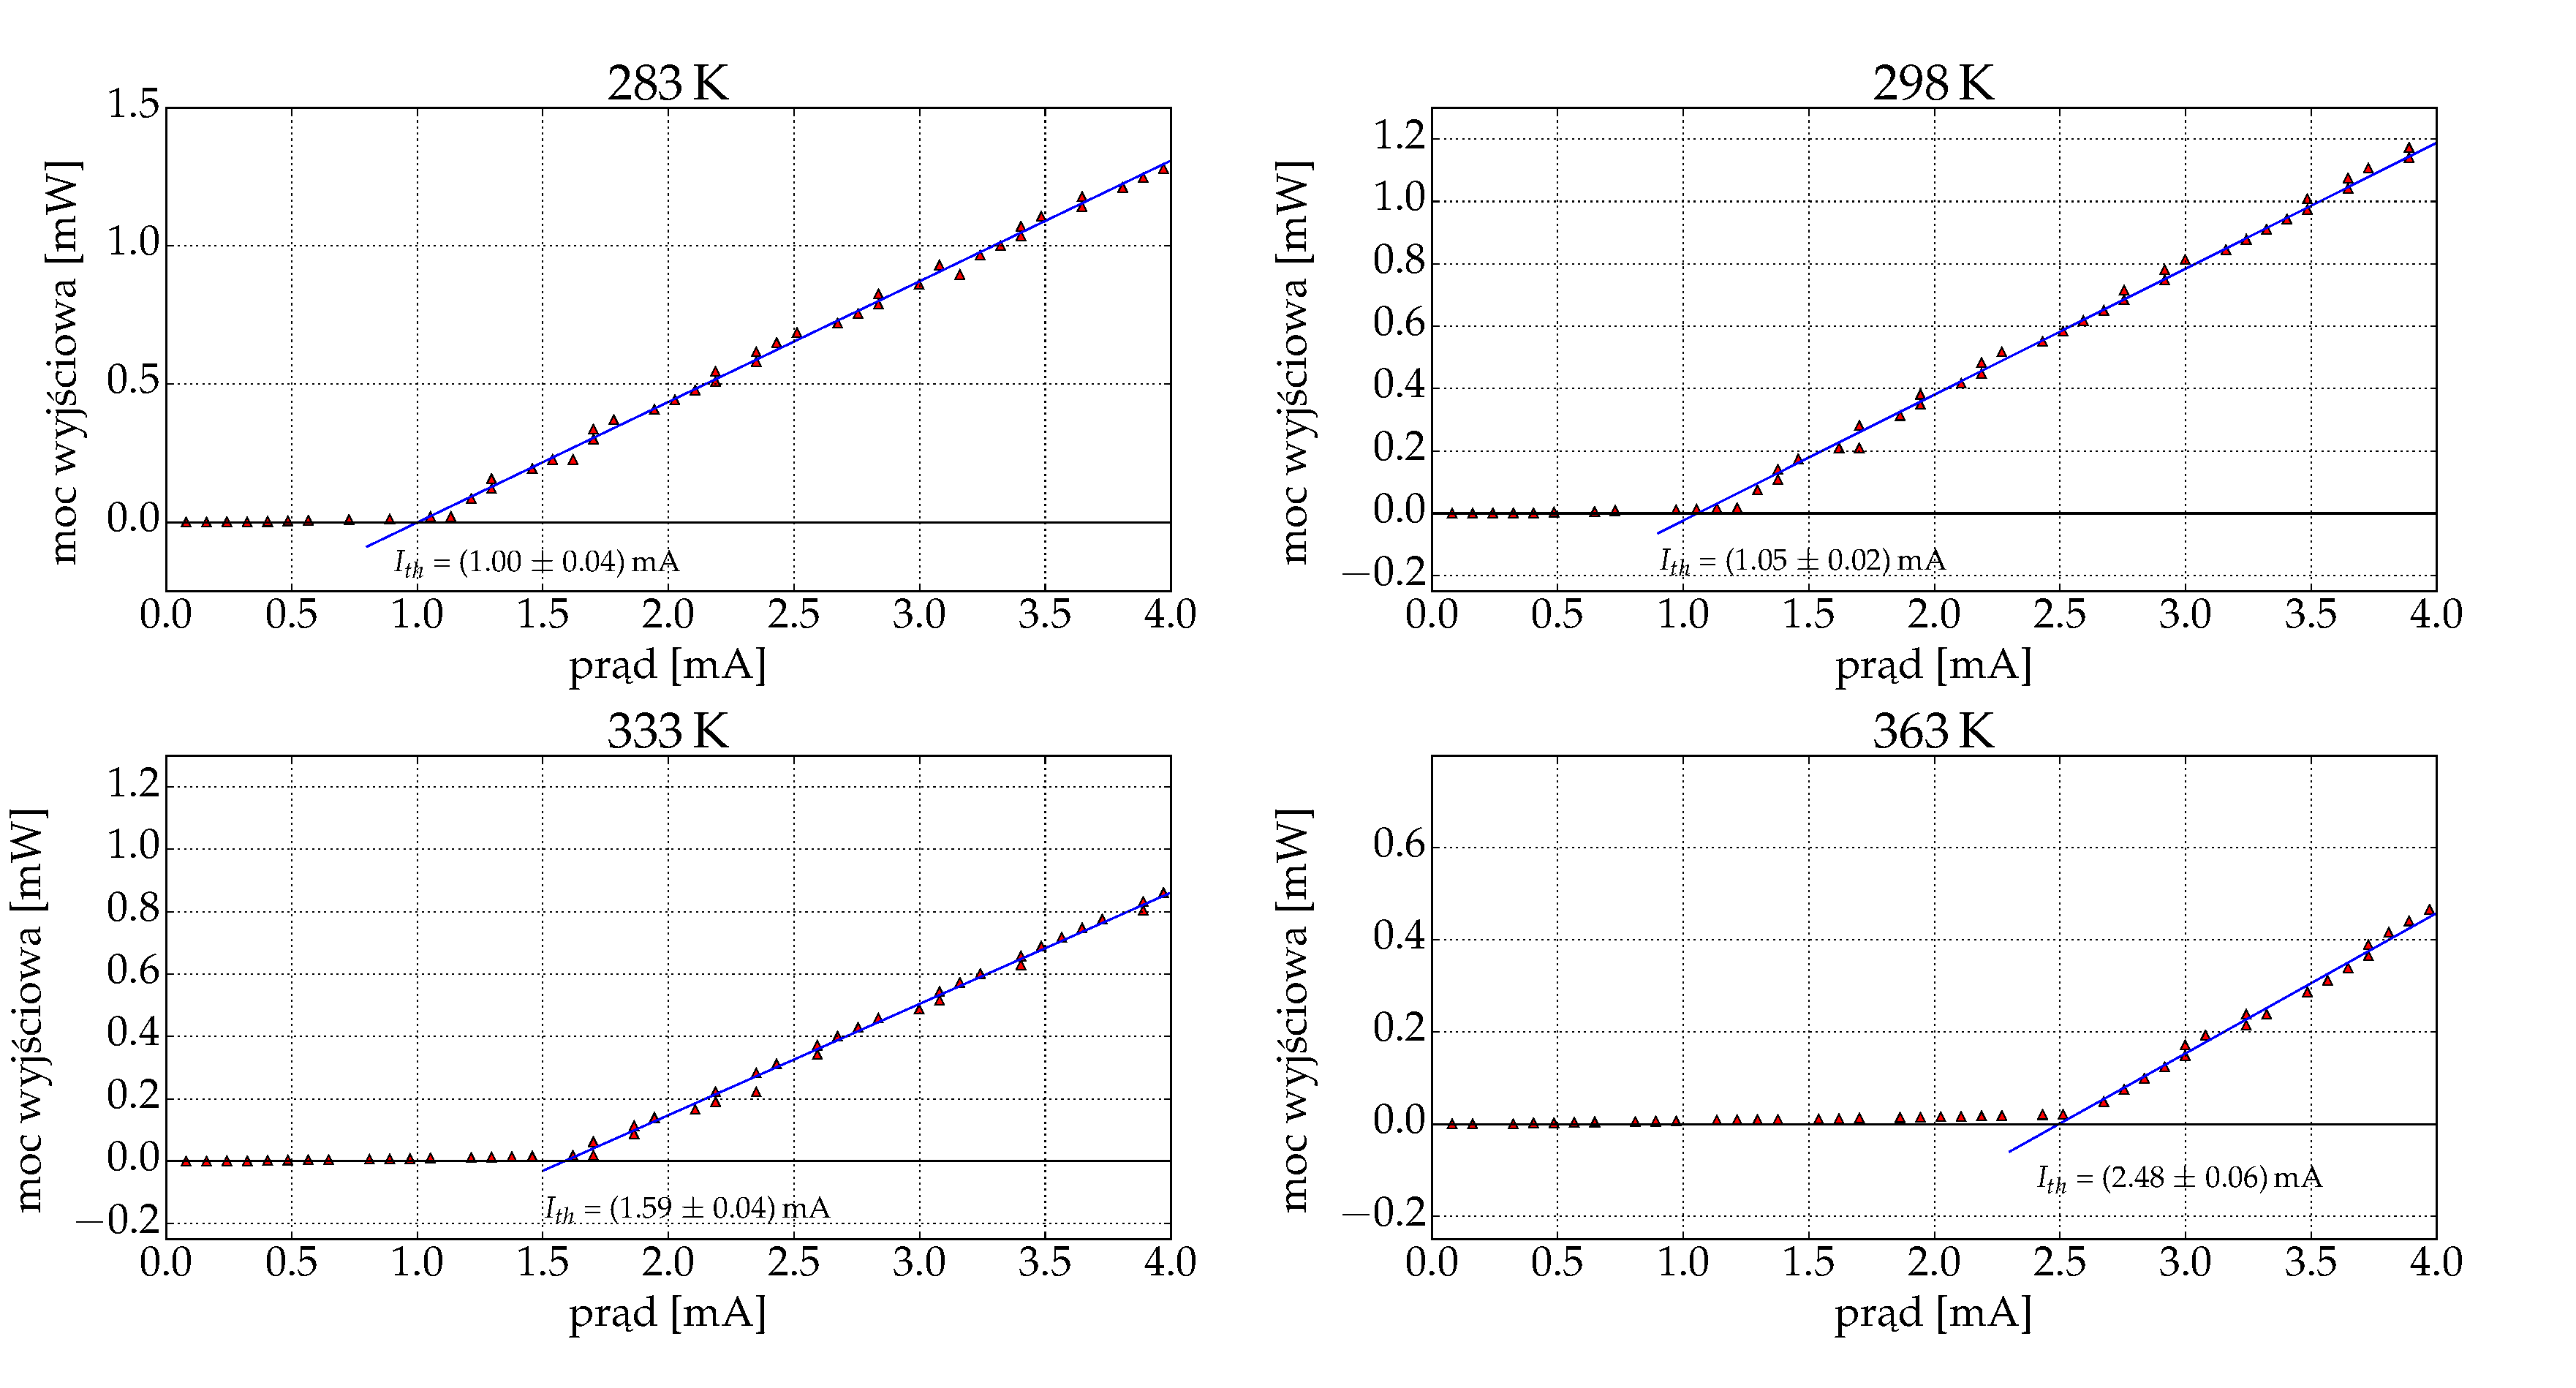
\includegraphics[scale=0.30]{plot980/plot_fit_i_th4.eps}
  \caption{Wykres ilustrujący wyznaczanie prądu progow dla lasera VCSEL 980\,nm.}
  \label{fig:plot_fit_i_th4_980}
\end{figure}
\begin{figure}
\center
  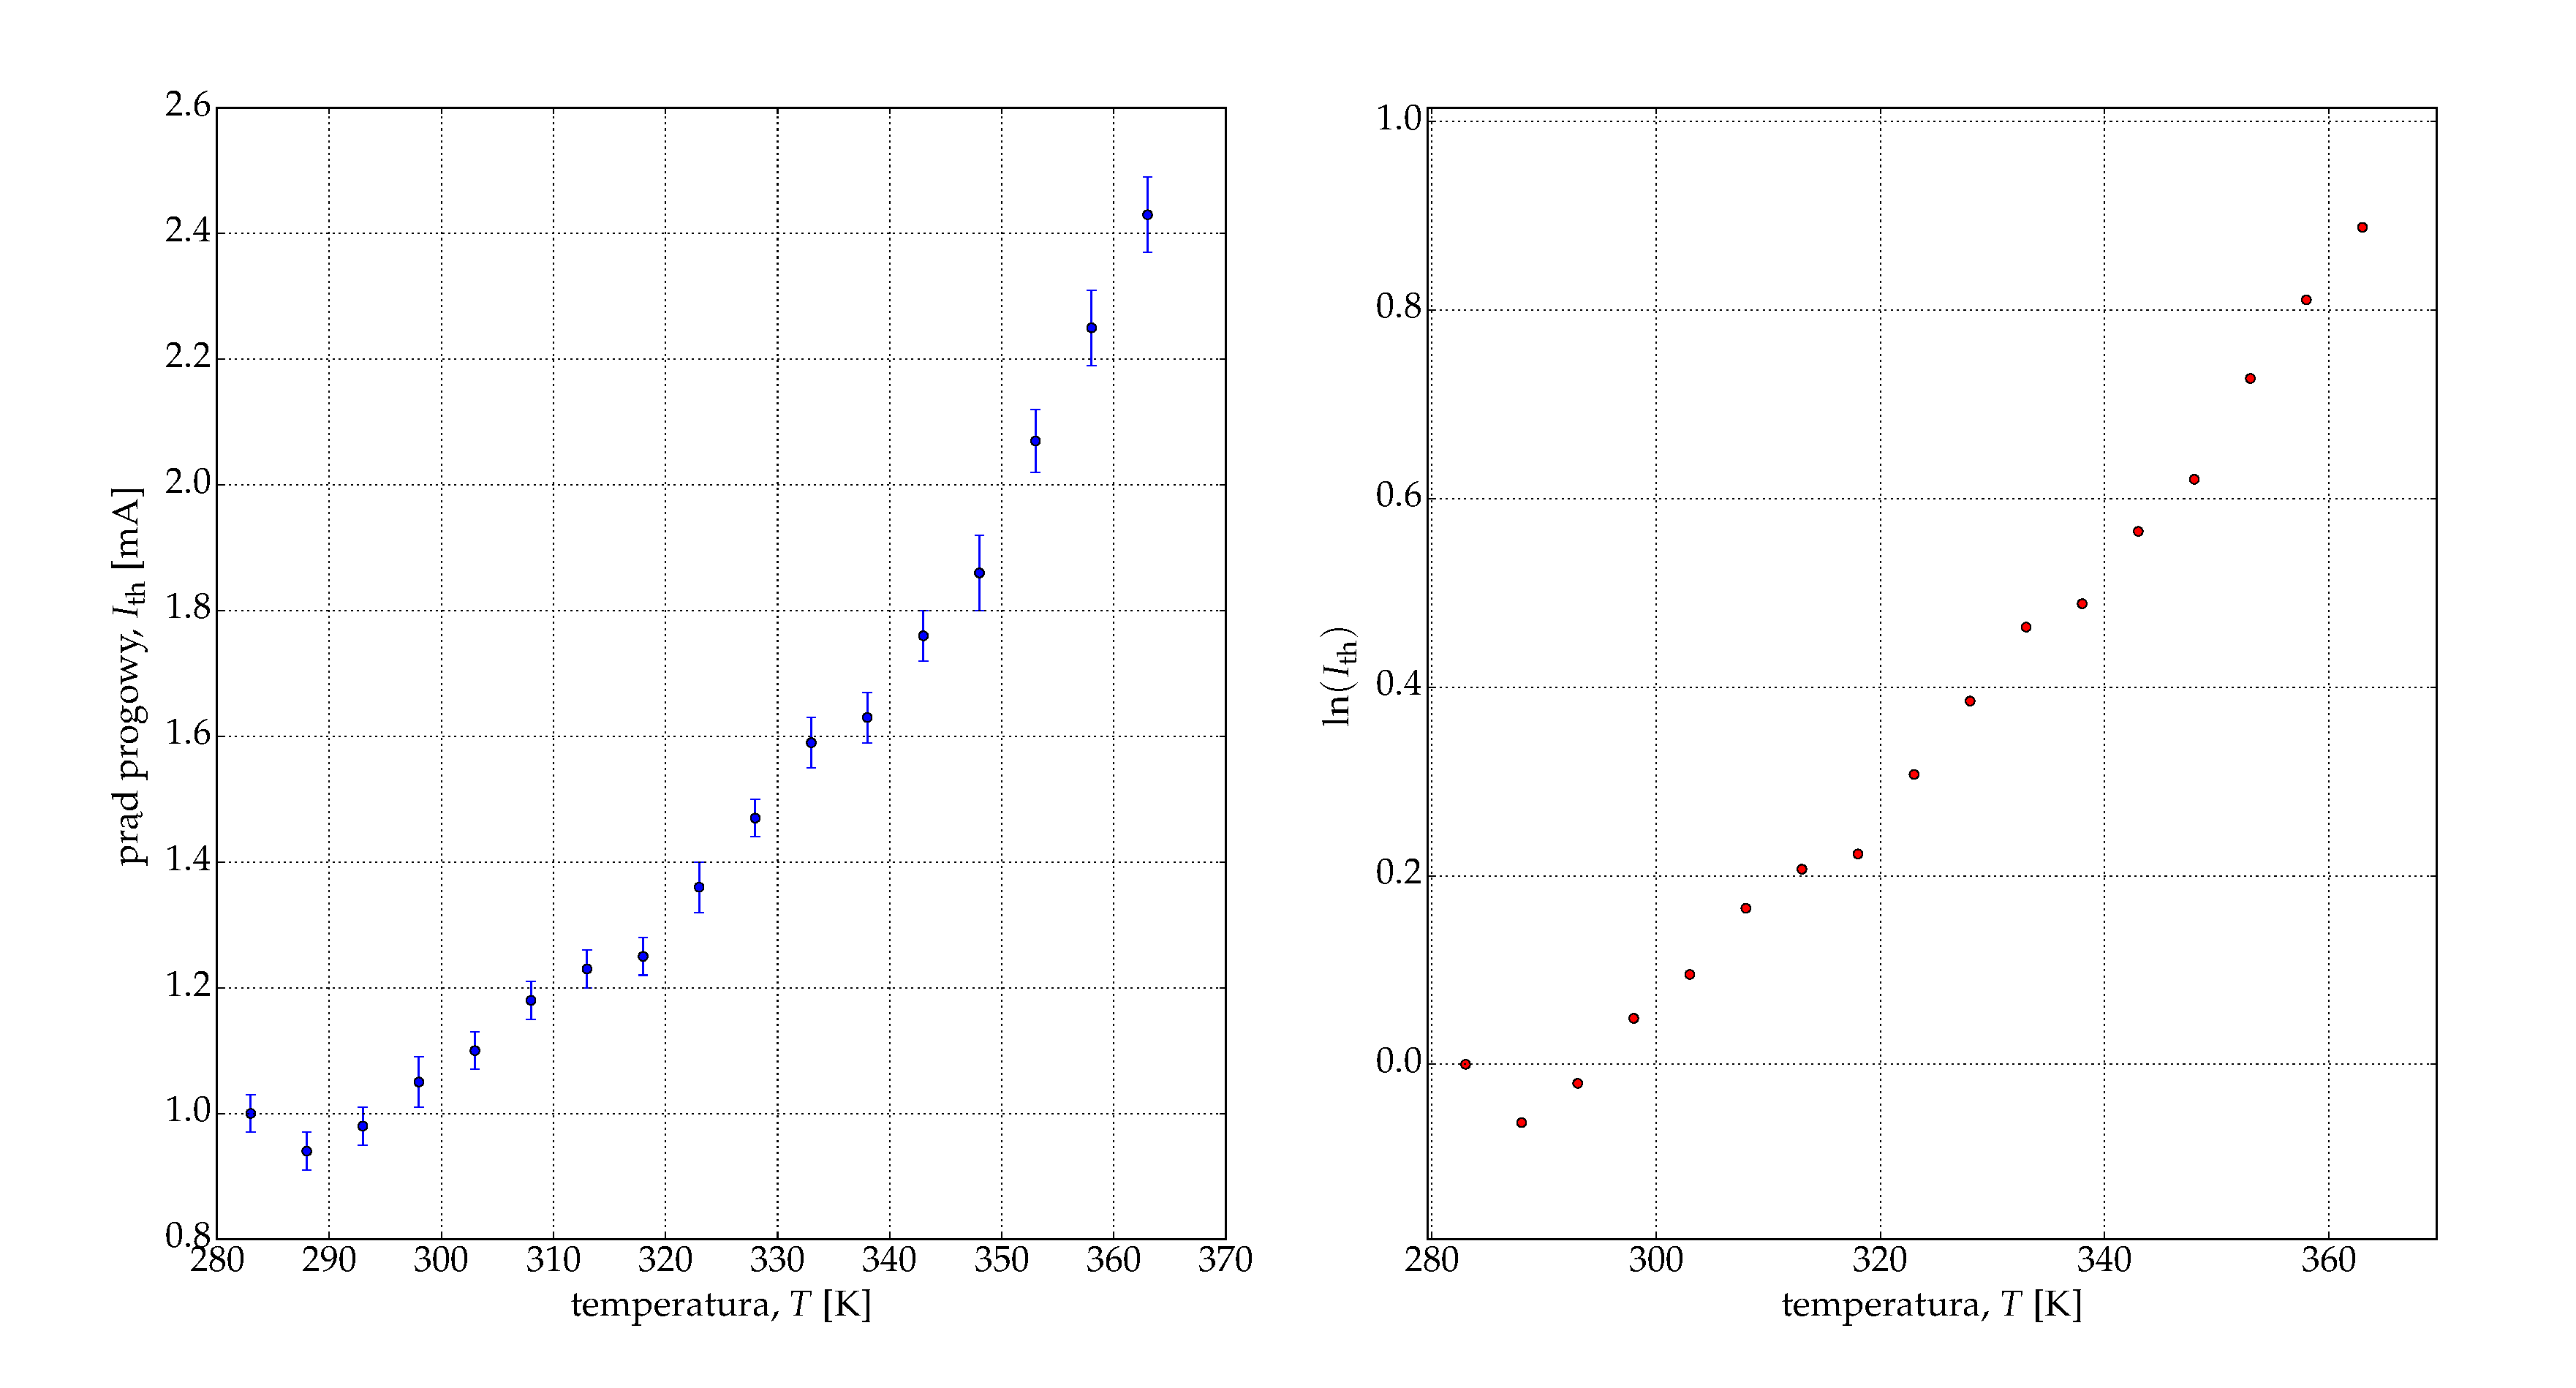
\includegraphics[scale=0.30]{plot980/plot_temp_i_th_log_lin.eps}
  \caption{Wykres prądu progow od temperatury dla lasera VCSEL 980\,nm w skali liniowej oraz logarytmicznej.}
  \label{fig:plot_temp_i_th_log_lin_980}
\end{figure}
\begin{figure}
\center
  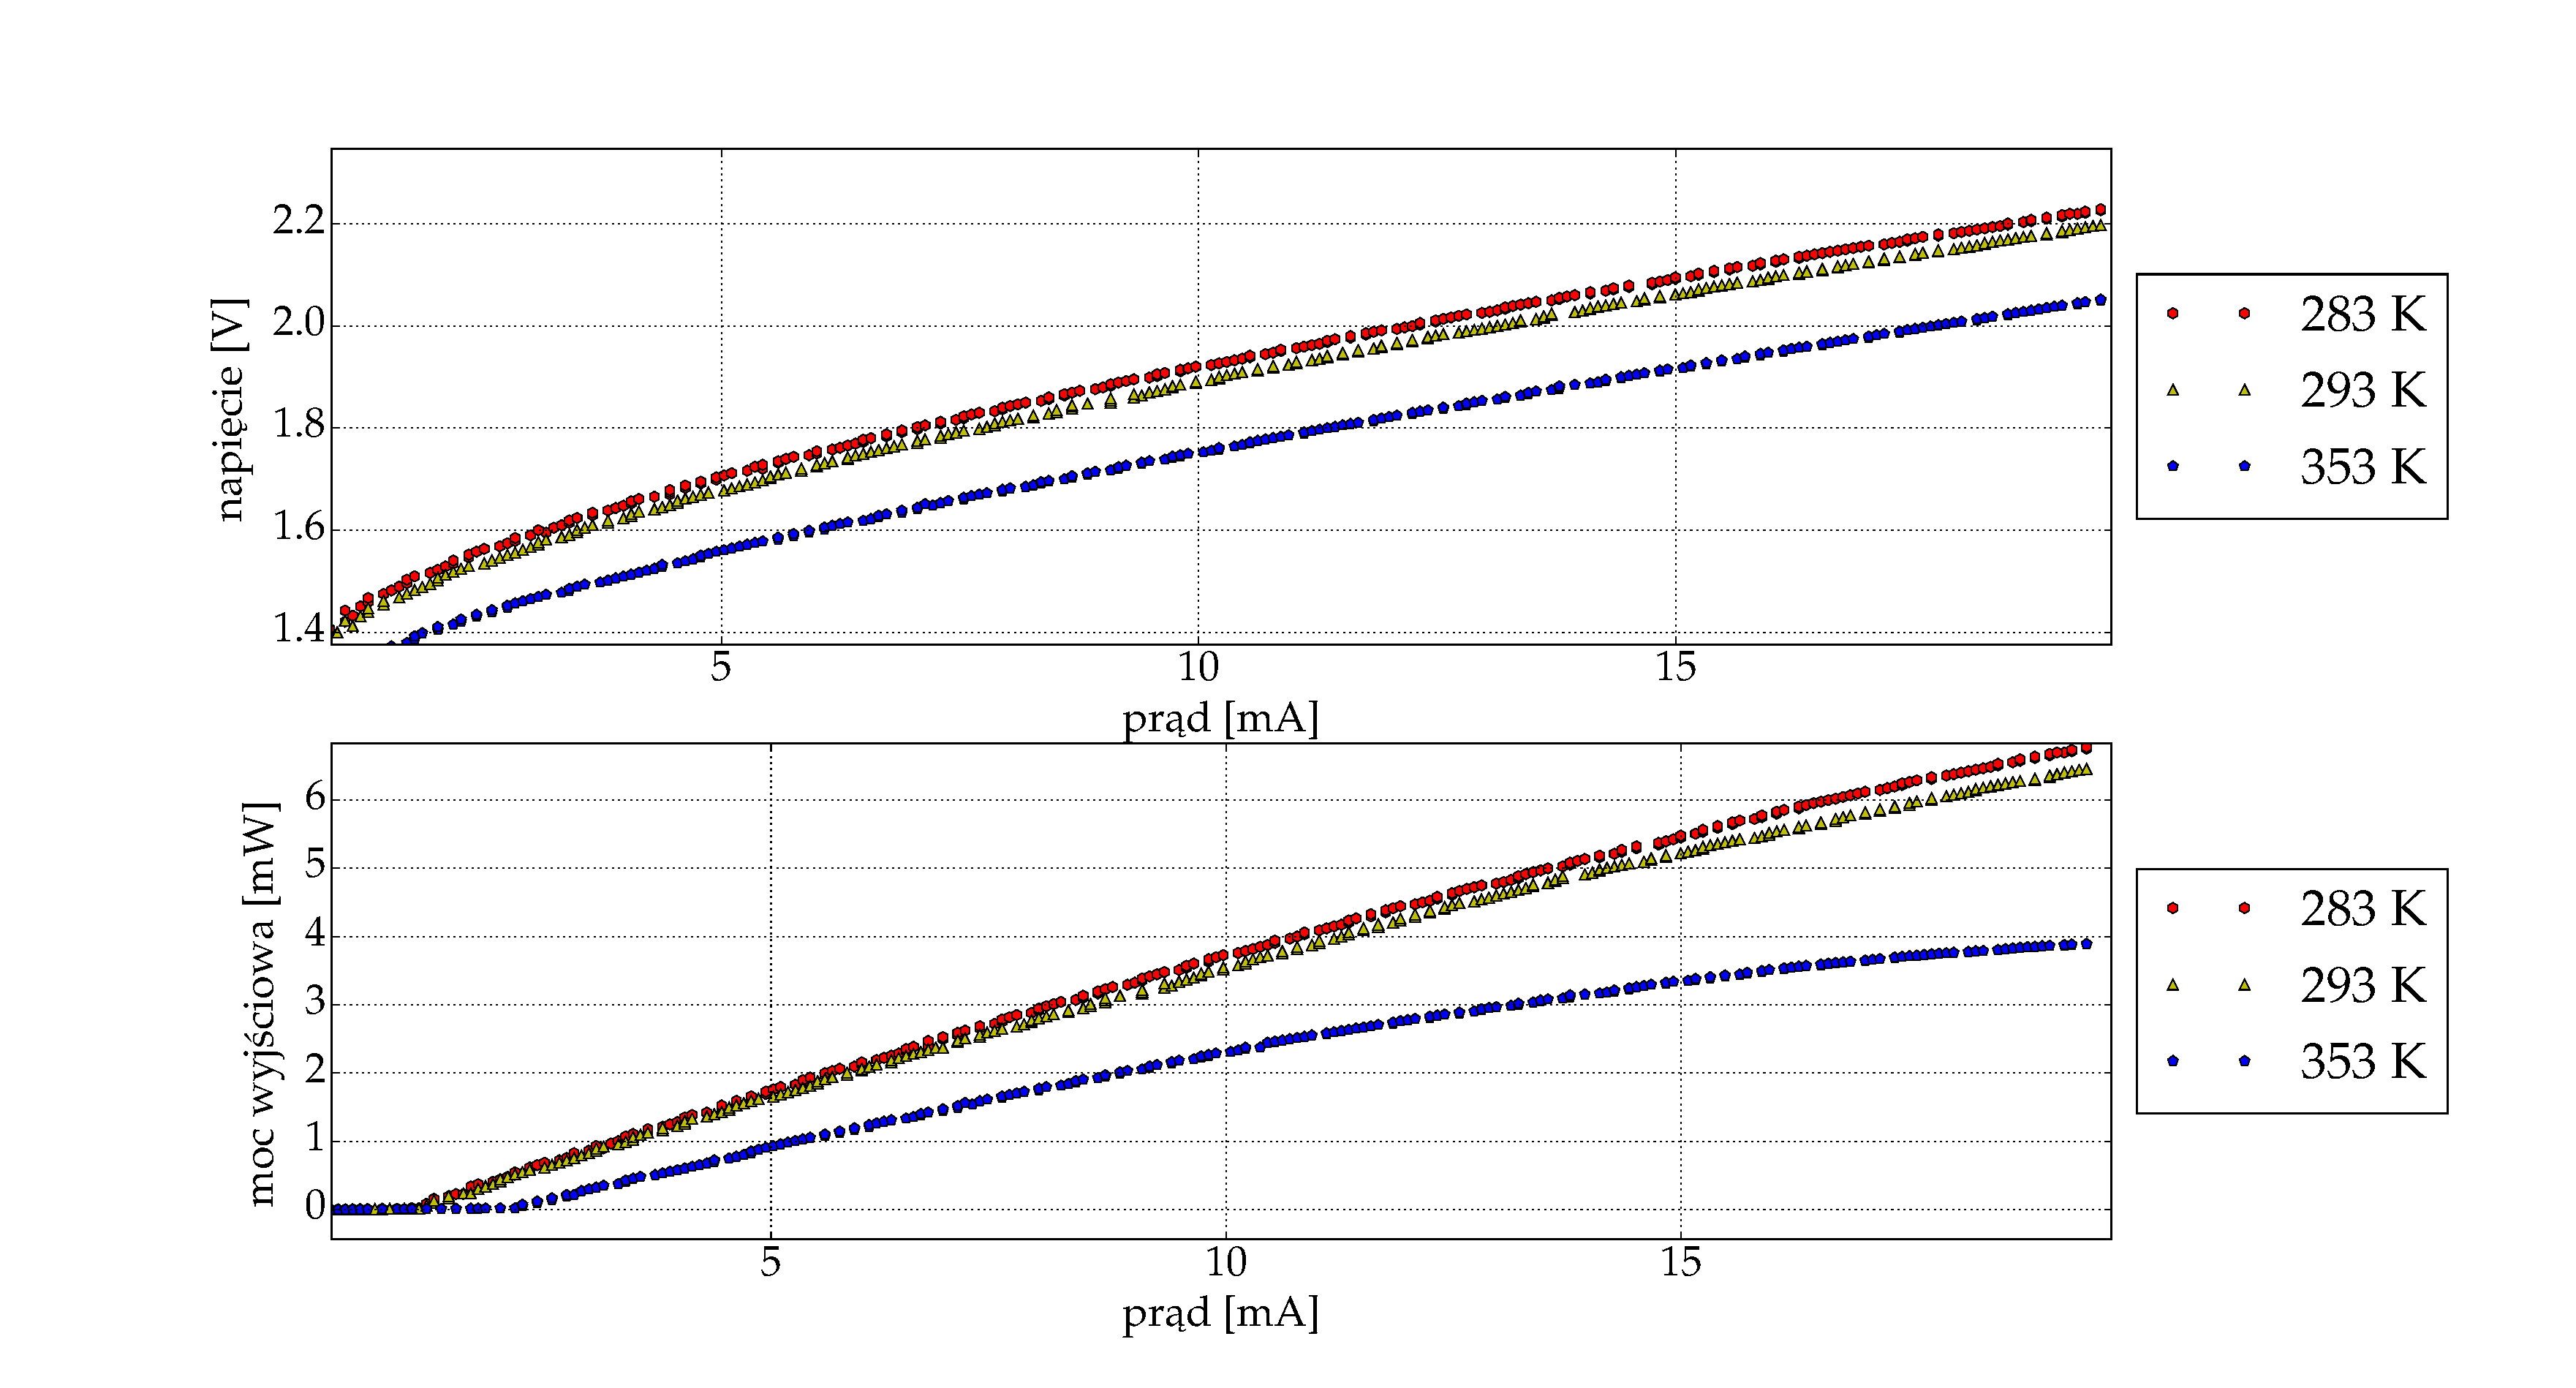
\includegraphics[scale=0.30]{plot980/plot_i_v_i_l.eps}
  \caption{Wykres napięcia oraz mocy wyjściowej w fukcji prądu dla lasera VCSEL 980\,nm.}
  \label{fig:plot_i_v_i_l_980}
\end{figure}
\begin{figure}
\center
  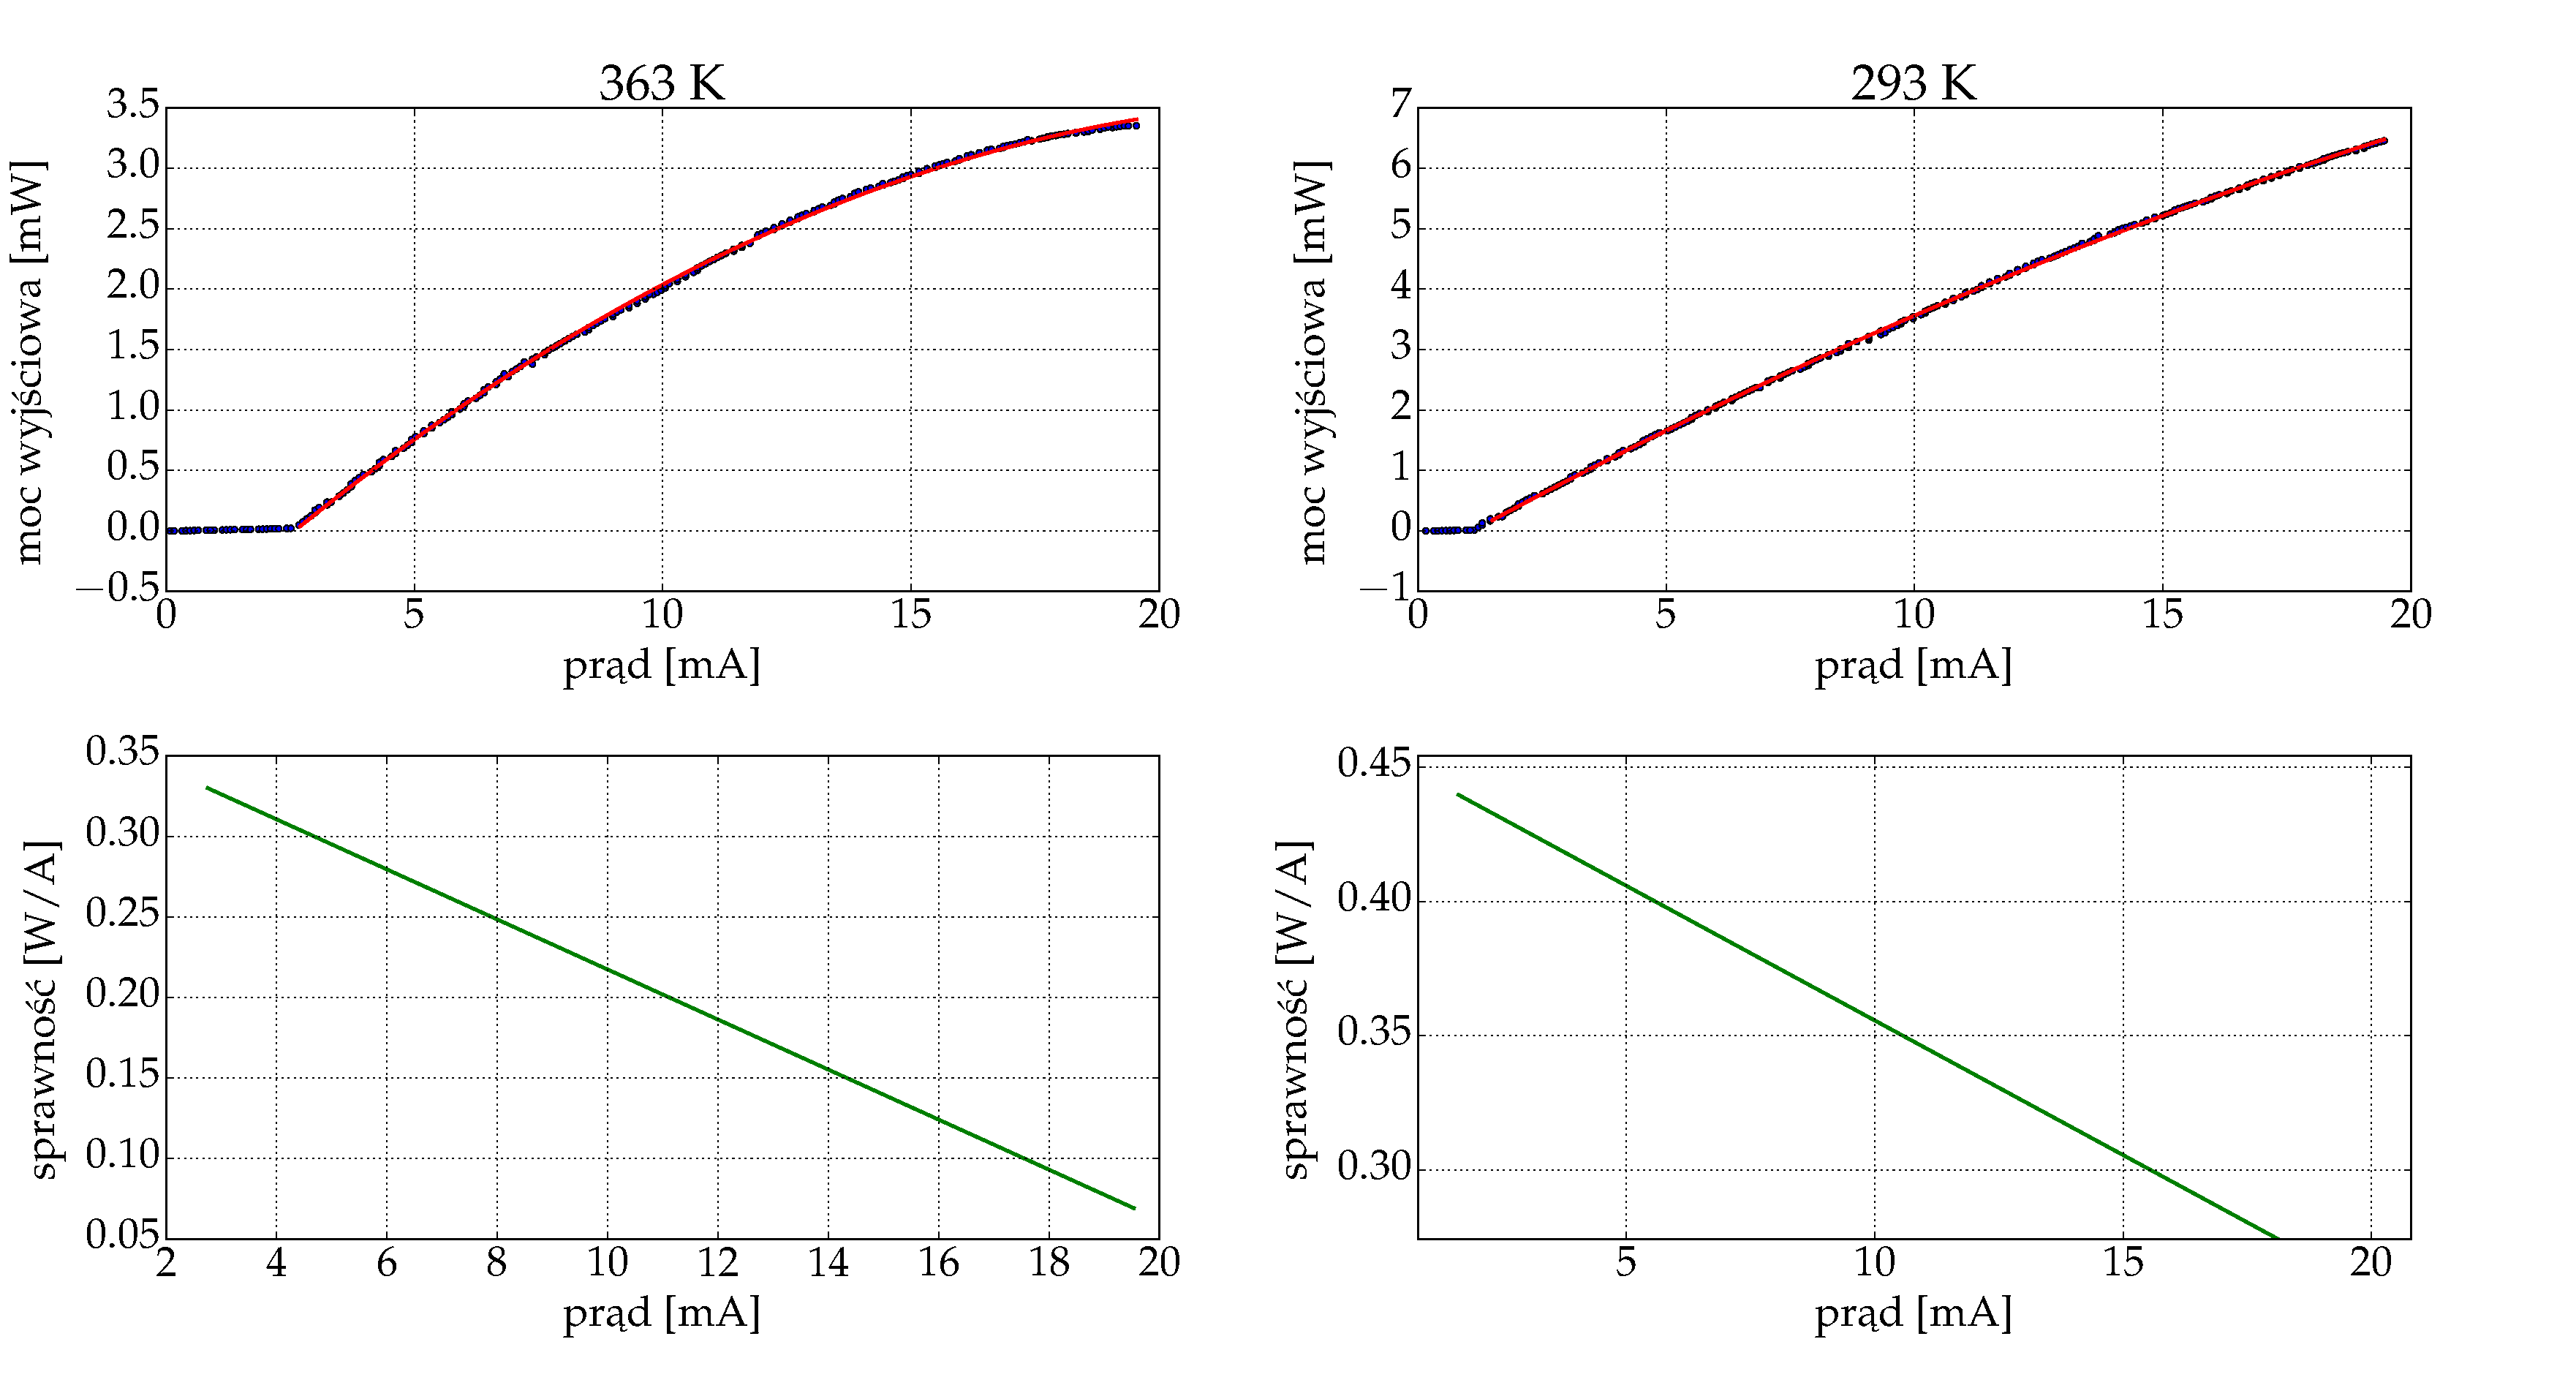
\includegraphics[scale=0.30]{plot980/plot_eff_via_current4.eps}
  \caption{Wykres sprawności różnoczkowej dla lasera VCSEL 980\,nm w dwóch różnych temperaturach.}
  \label{fig:plot_eff_via_current4_980}
\end{figure}
\begin{figure}
\center
  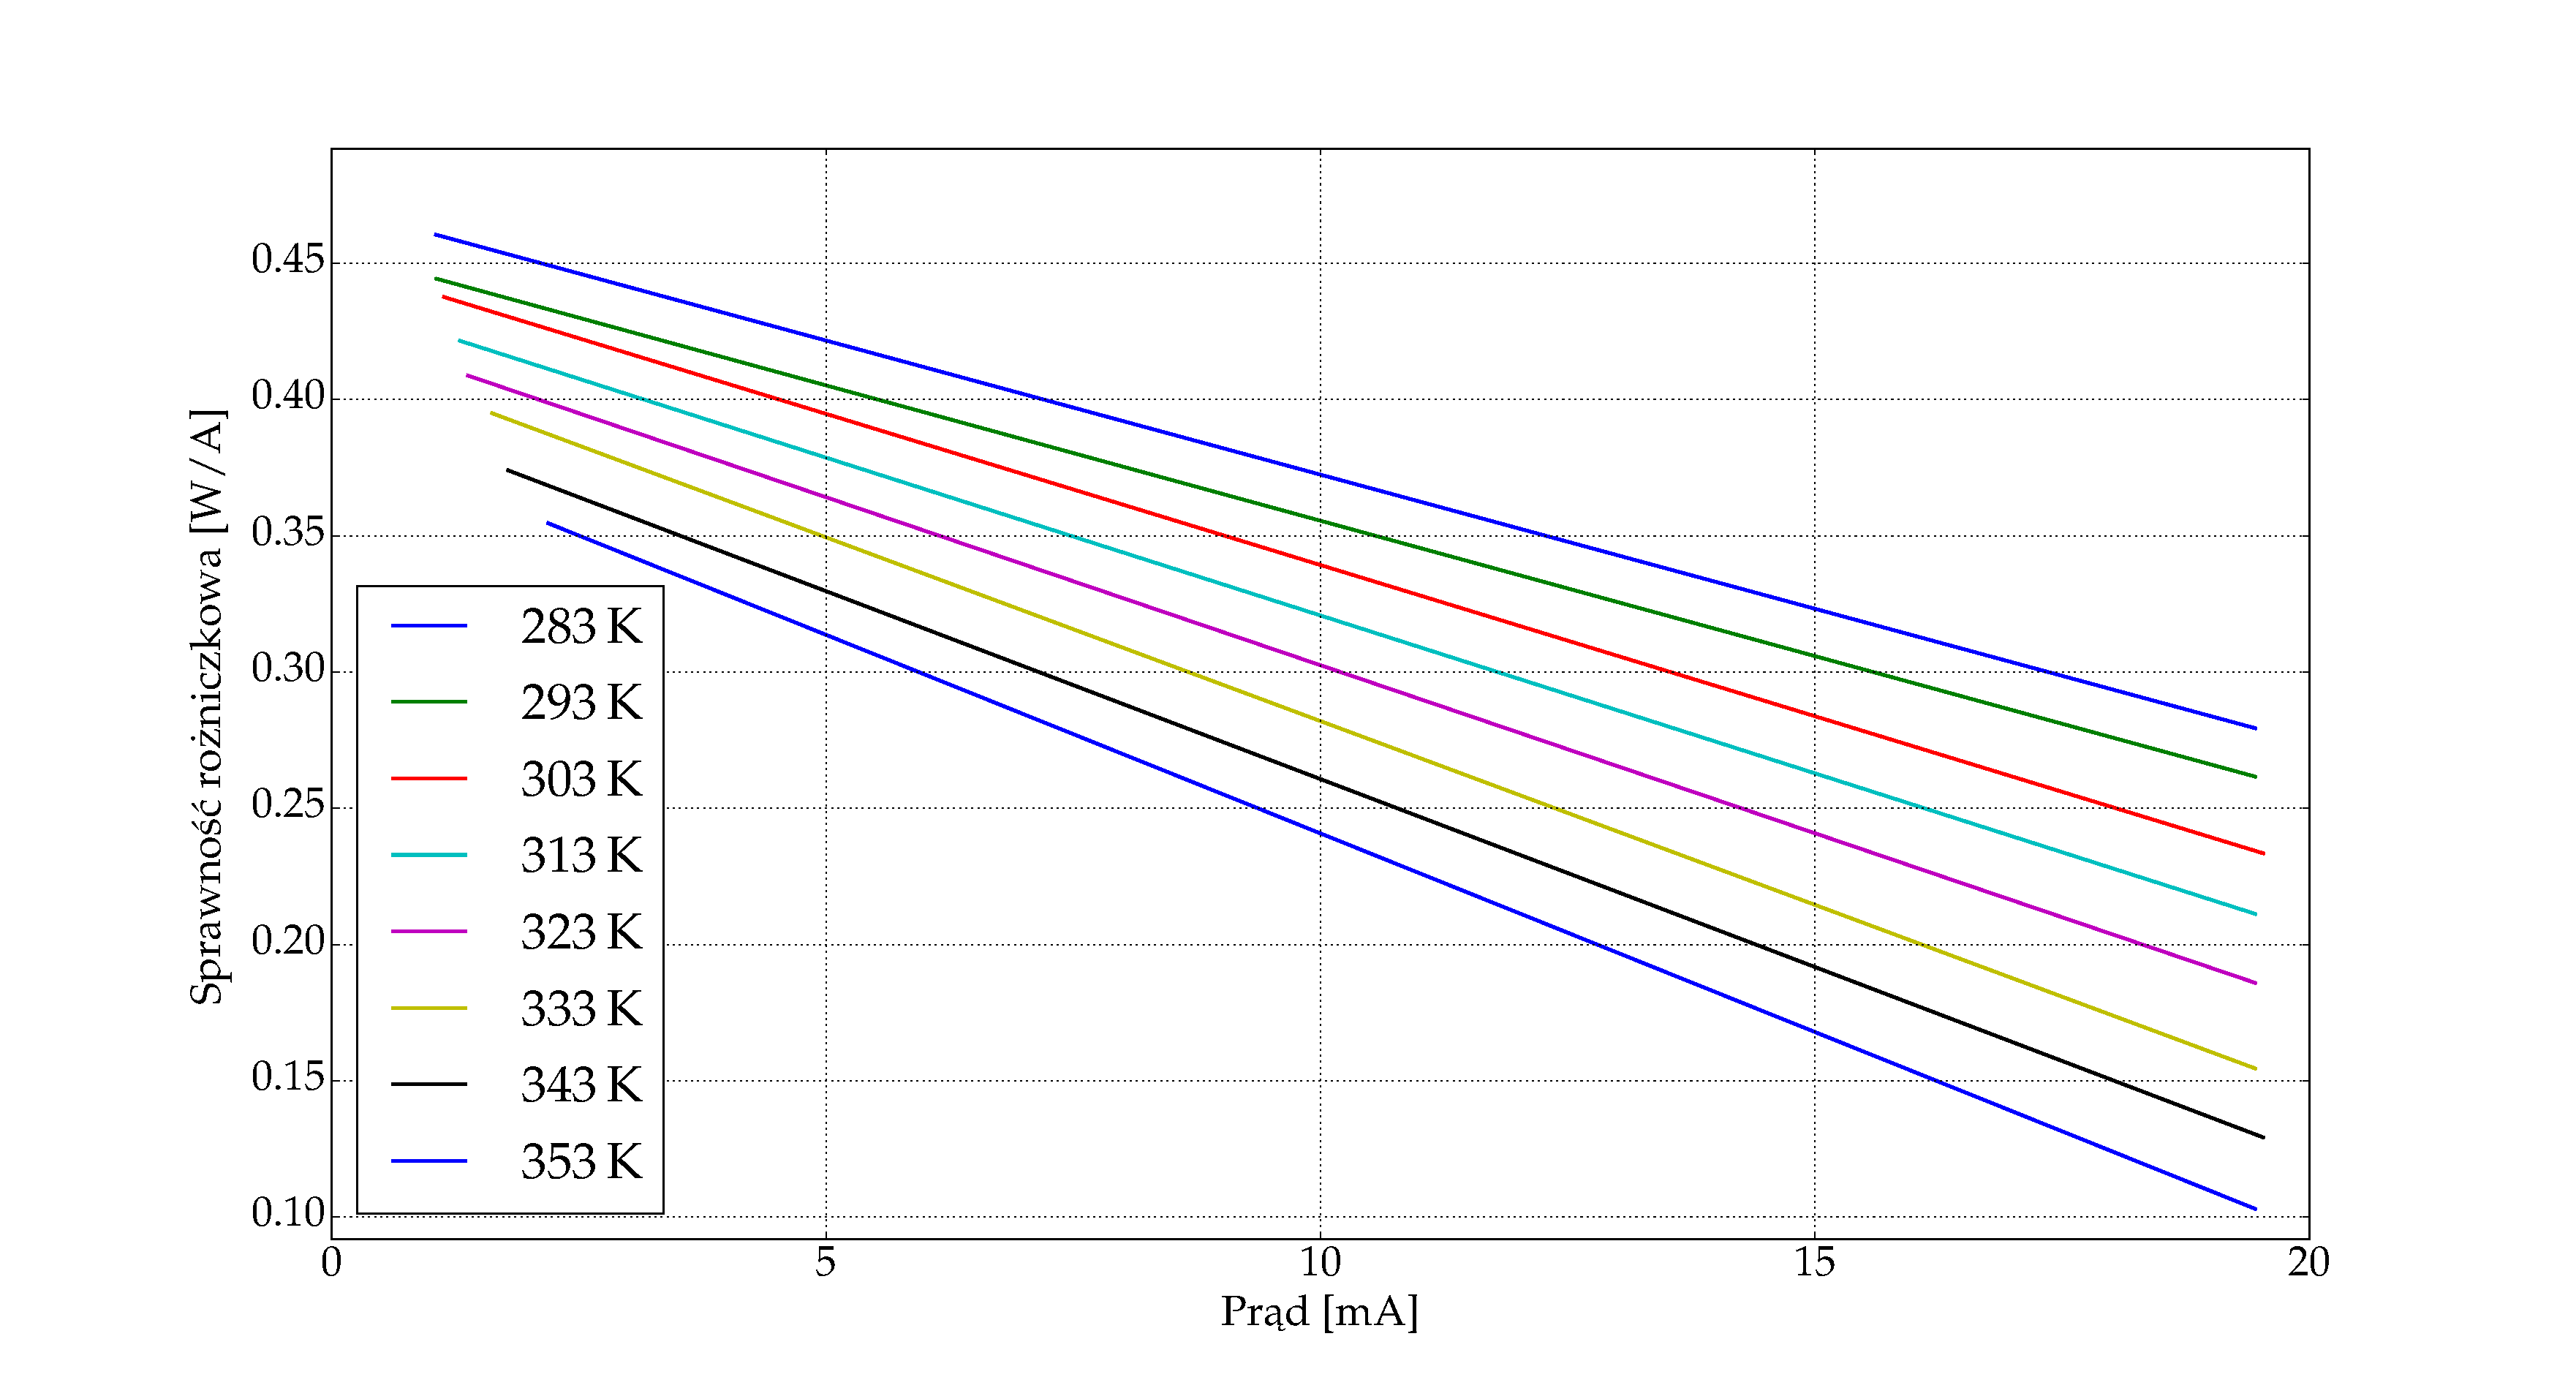
\includegraphics[scale=0.25]{plot980/plot_eff_via_current_all.eps}
  \caption{Wykres sprawności różniczkowej dla lasera VCSEL 980\,nm w różnych temperaturach.}
  \label{fig:plot_eff_via_current_all_980}
\end{figure}
\newpage
\section{Porównanie laserów}
Analizując pomiary dla 4 laserów które przeprowadziłem, można wyciągnąć nastepujące wnioski:
\begin{itemize}
\item Sprawność różniczkowa laserów krawędziowych w funkcji zarówno prądu i mocy wejściowej jest większa, co
przedstawia wykres na rysunku ~\ref{fig:plot_eff}
\item Prąd progowy dla laserów krawędziowych jest większy od prądu progowego dla laserów VCSEL, co przedstawia wykres
na rysunku~\ref{fig:plot_temp_i_th}.
\item Także, sprawność całkowita w wyższych temperaturach jest większa, co możemy zobaczyć na wykresie przedstawionym na
rysunku~\ref{fig:plot_wall_eff}.
\end{itemize}
\begin{figure}[H]
\center
  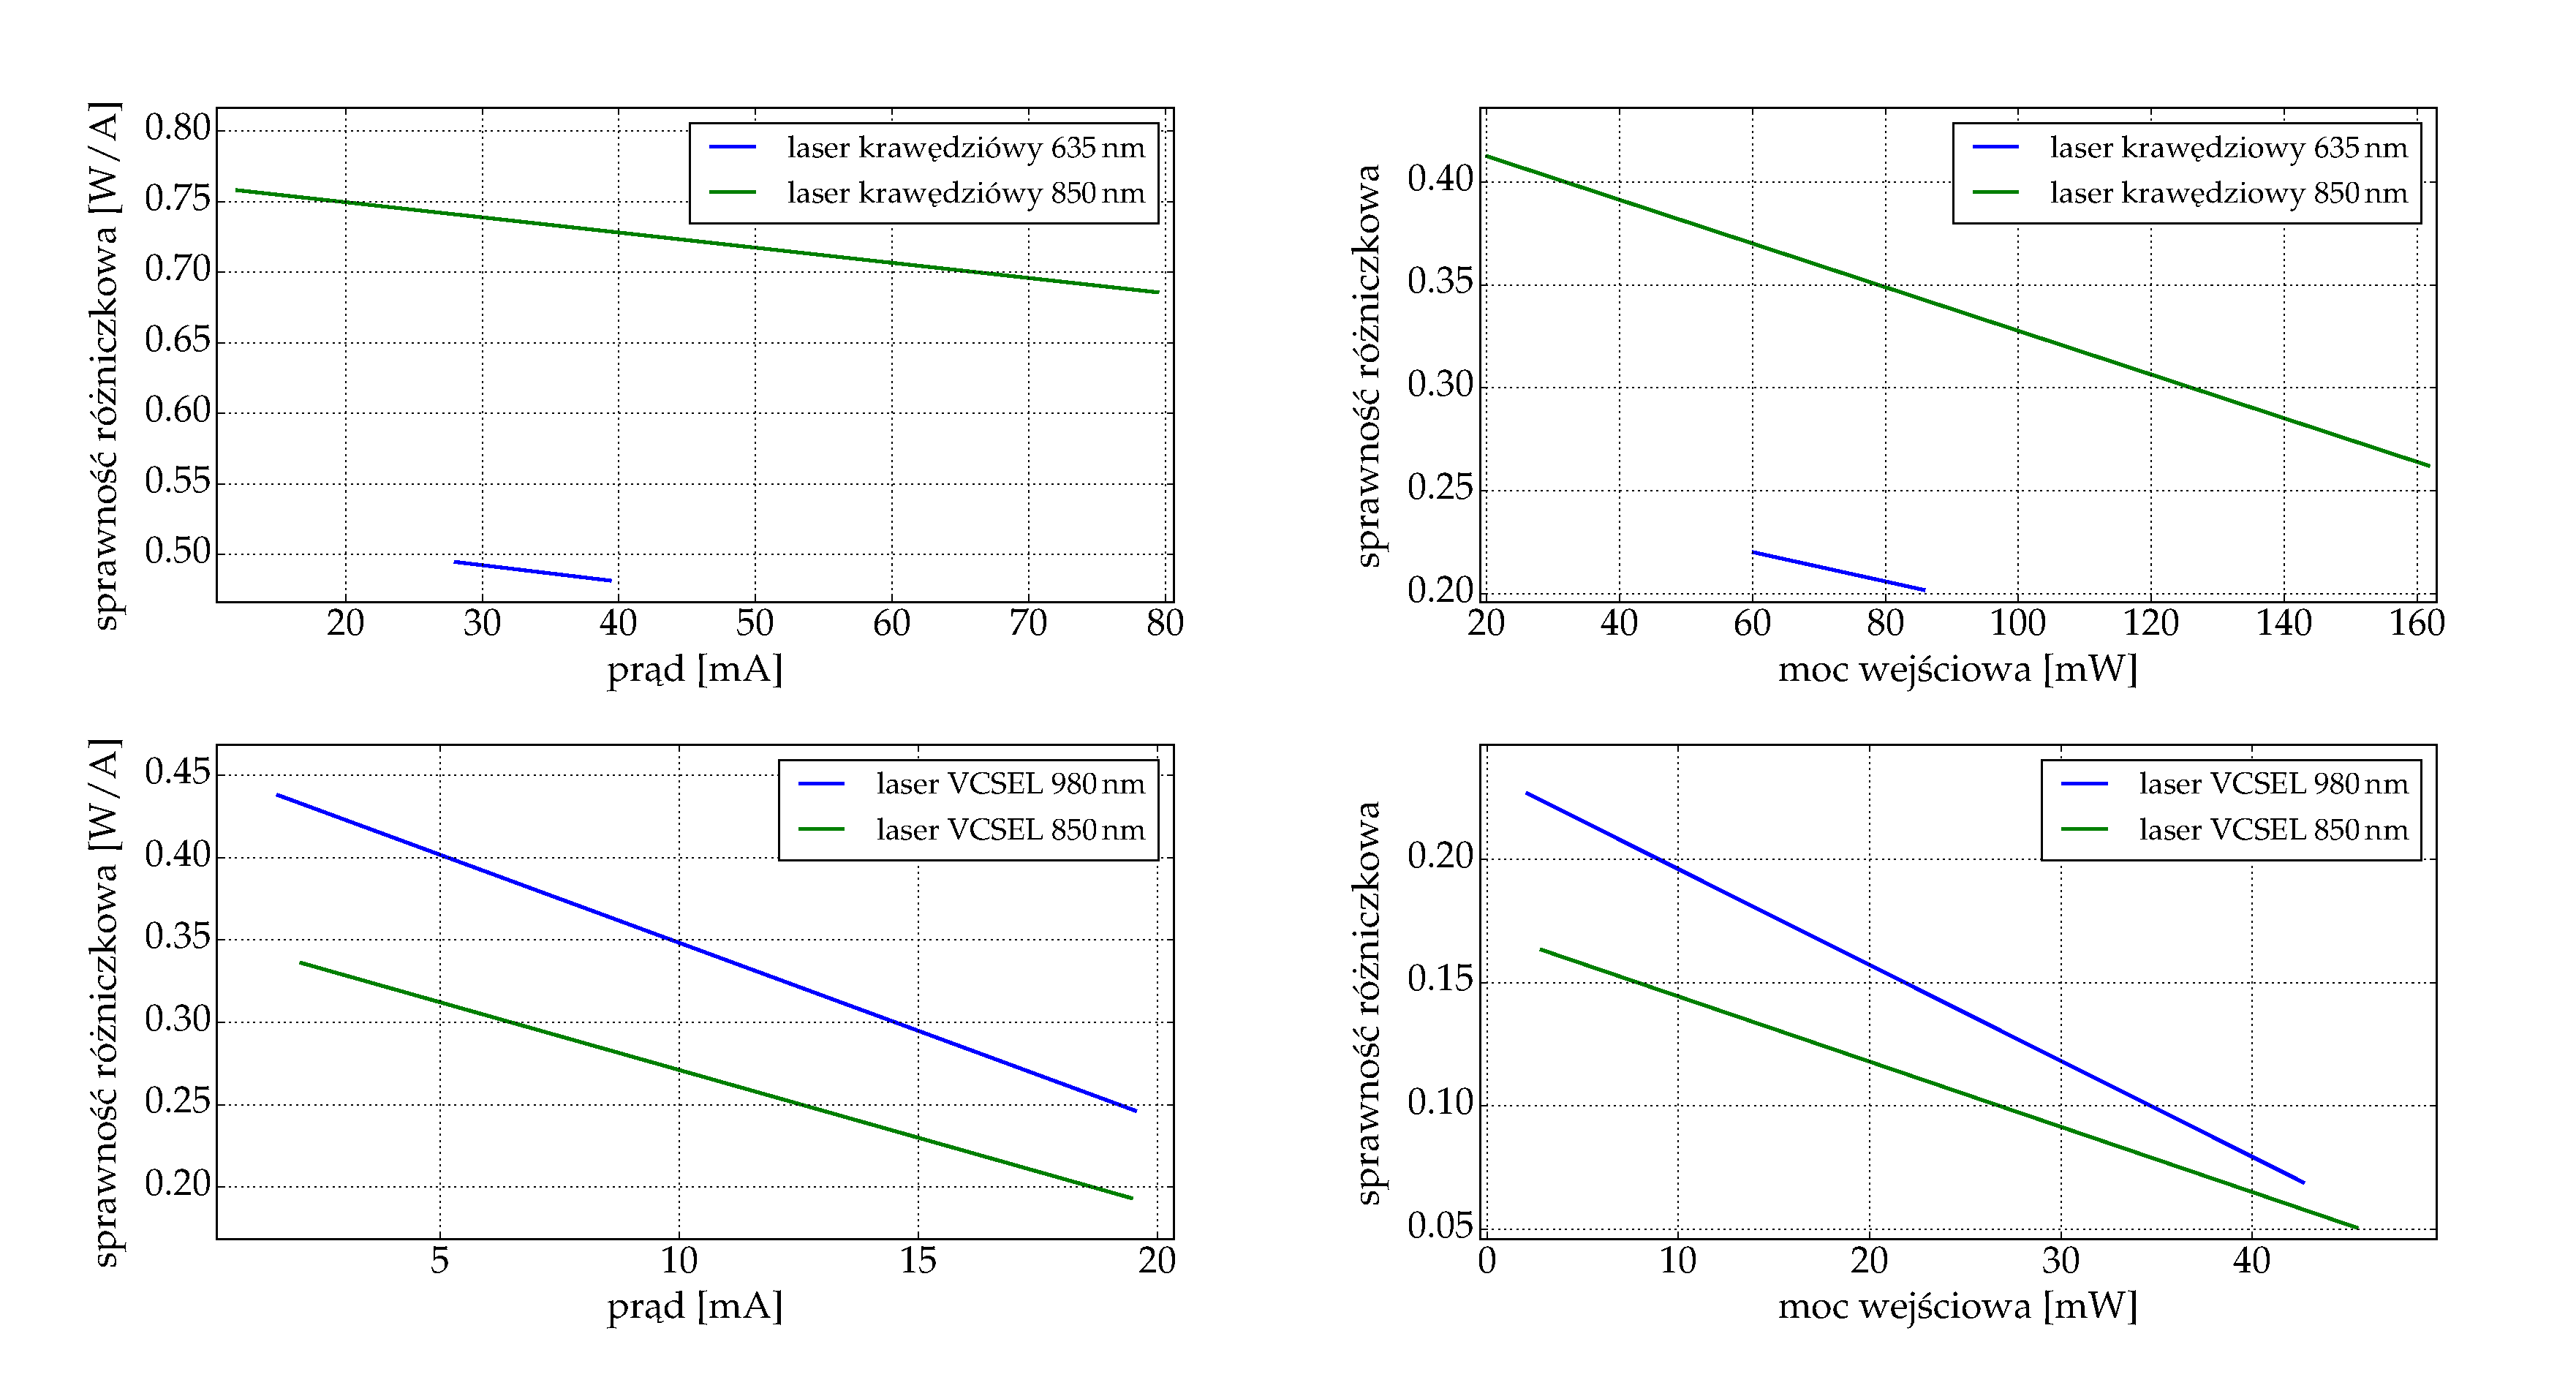
\includegraphics[scale=0.30]{plot_common/plot_eff.eps}
  \caption{Wykres sprawności różniczkowej w funkcji prądu oraz mocy wejściowej.}
  \label{fig:plot_eff}
\end{figure}
\begin{figure}
\center
  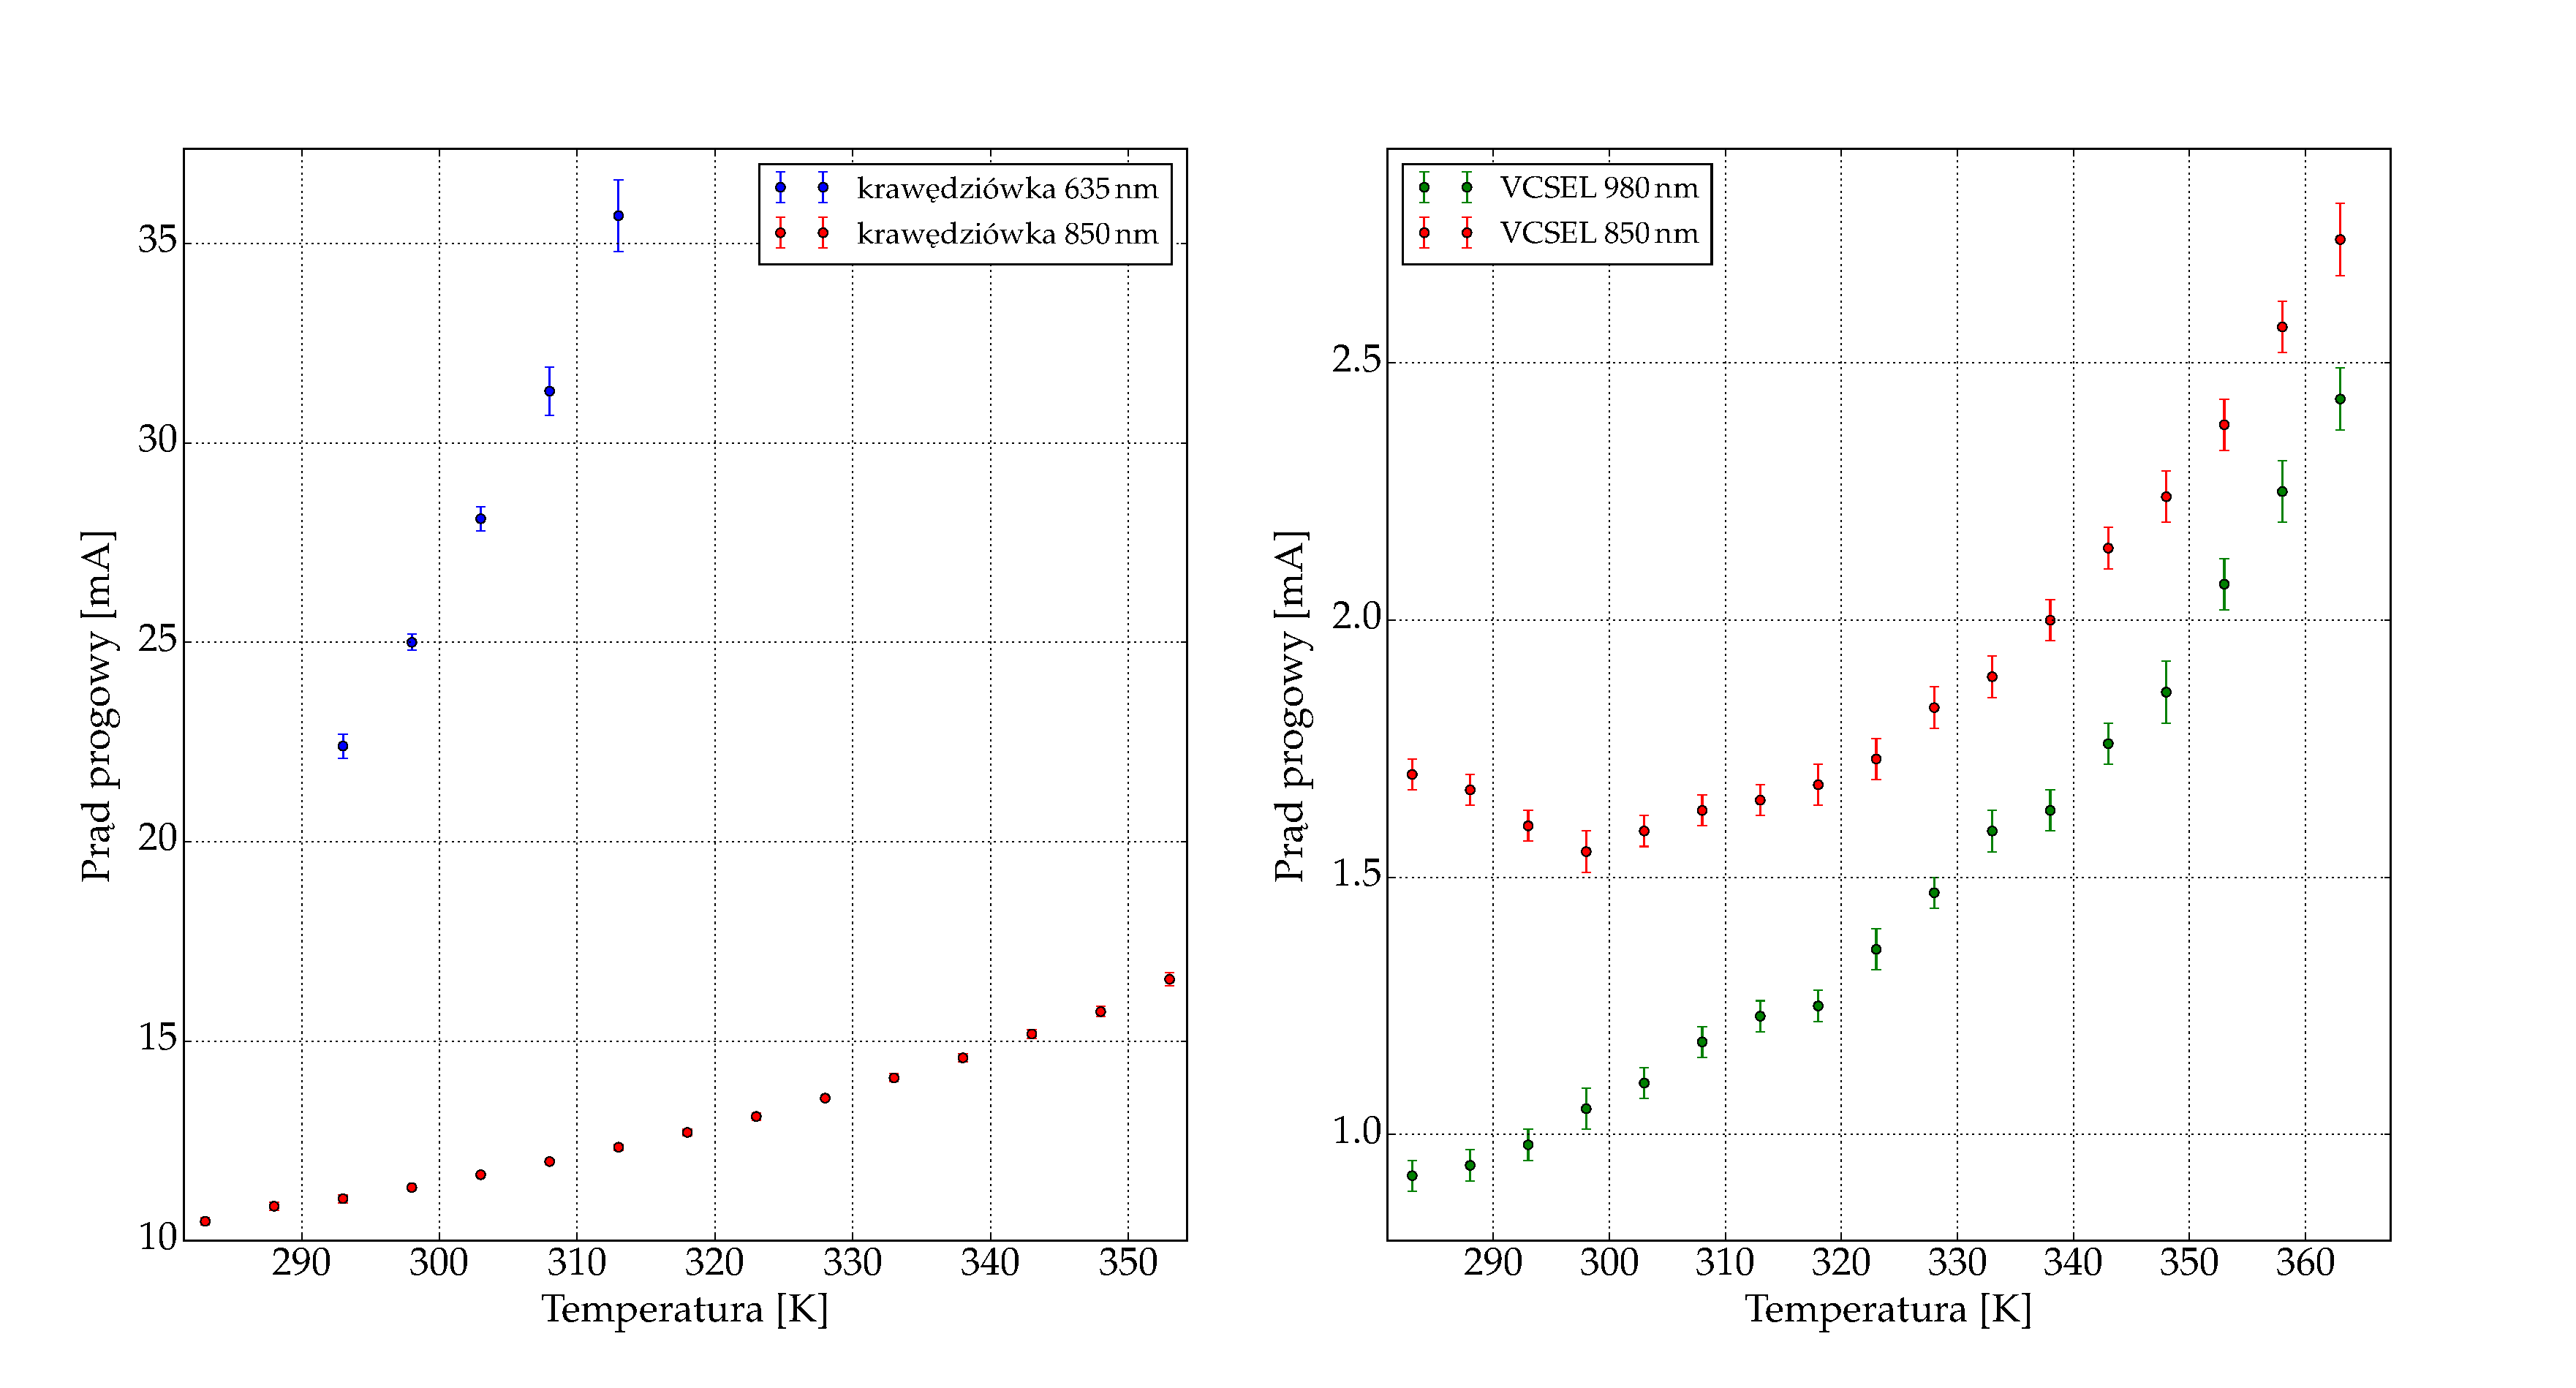
\includegraphics[scale=0.30]{plot_common/plot_temp_i_th.eps}
  \caption{Wykres prądu progowego od temperatury.}
  \label{fig:plot_temp_i_th}
\end{figure}
\begin{figure}
\center
  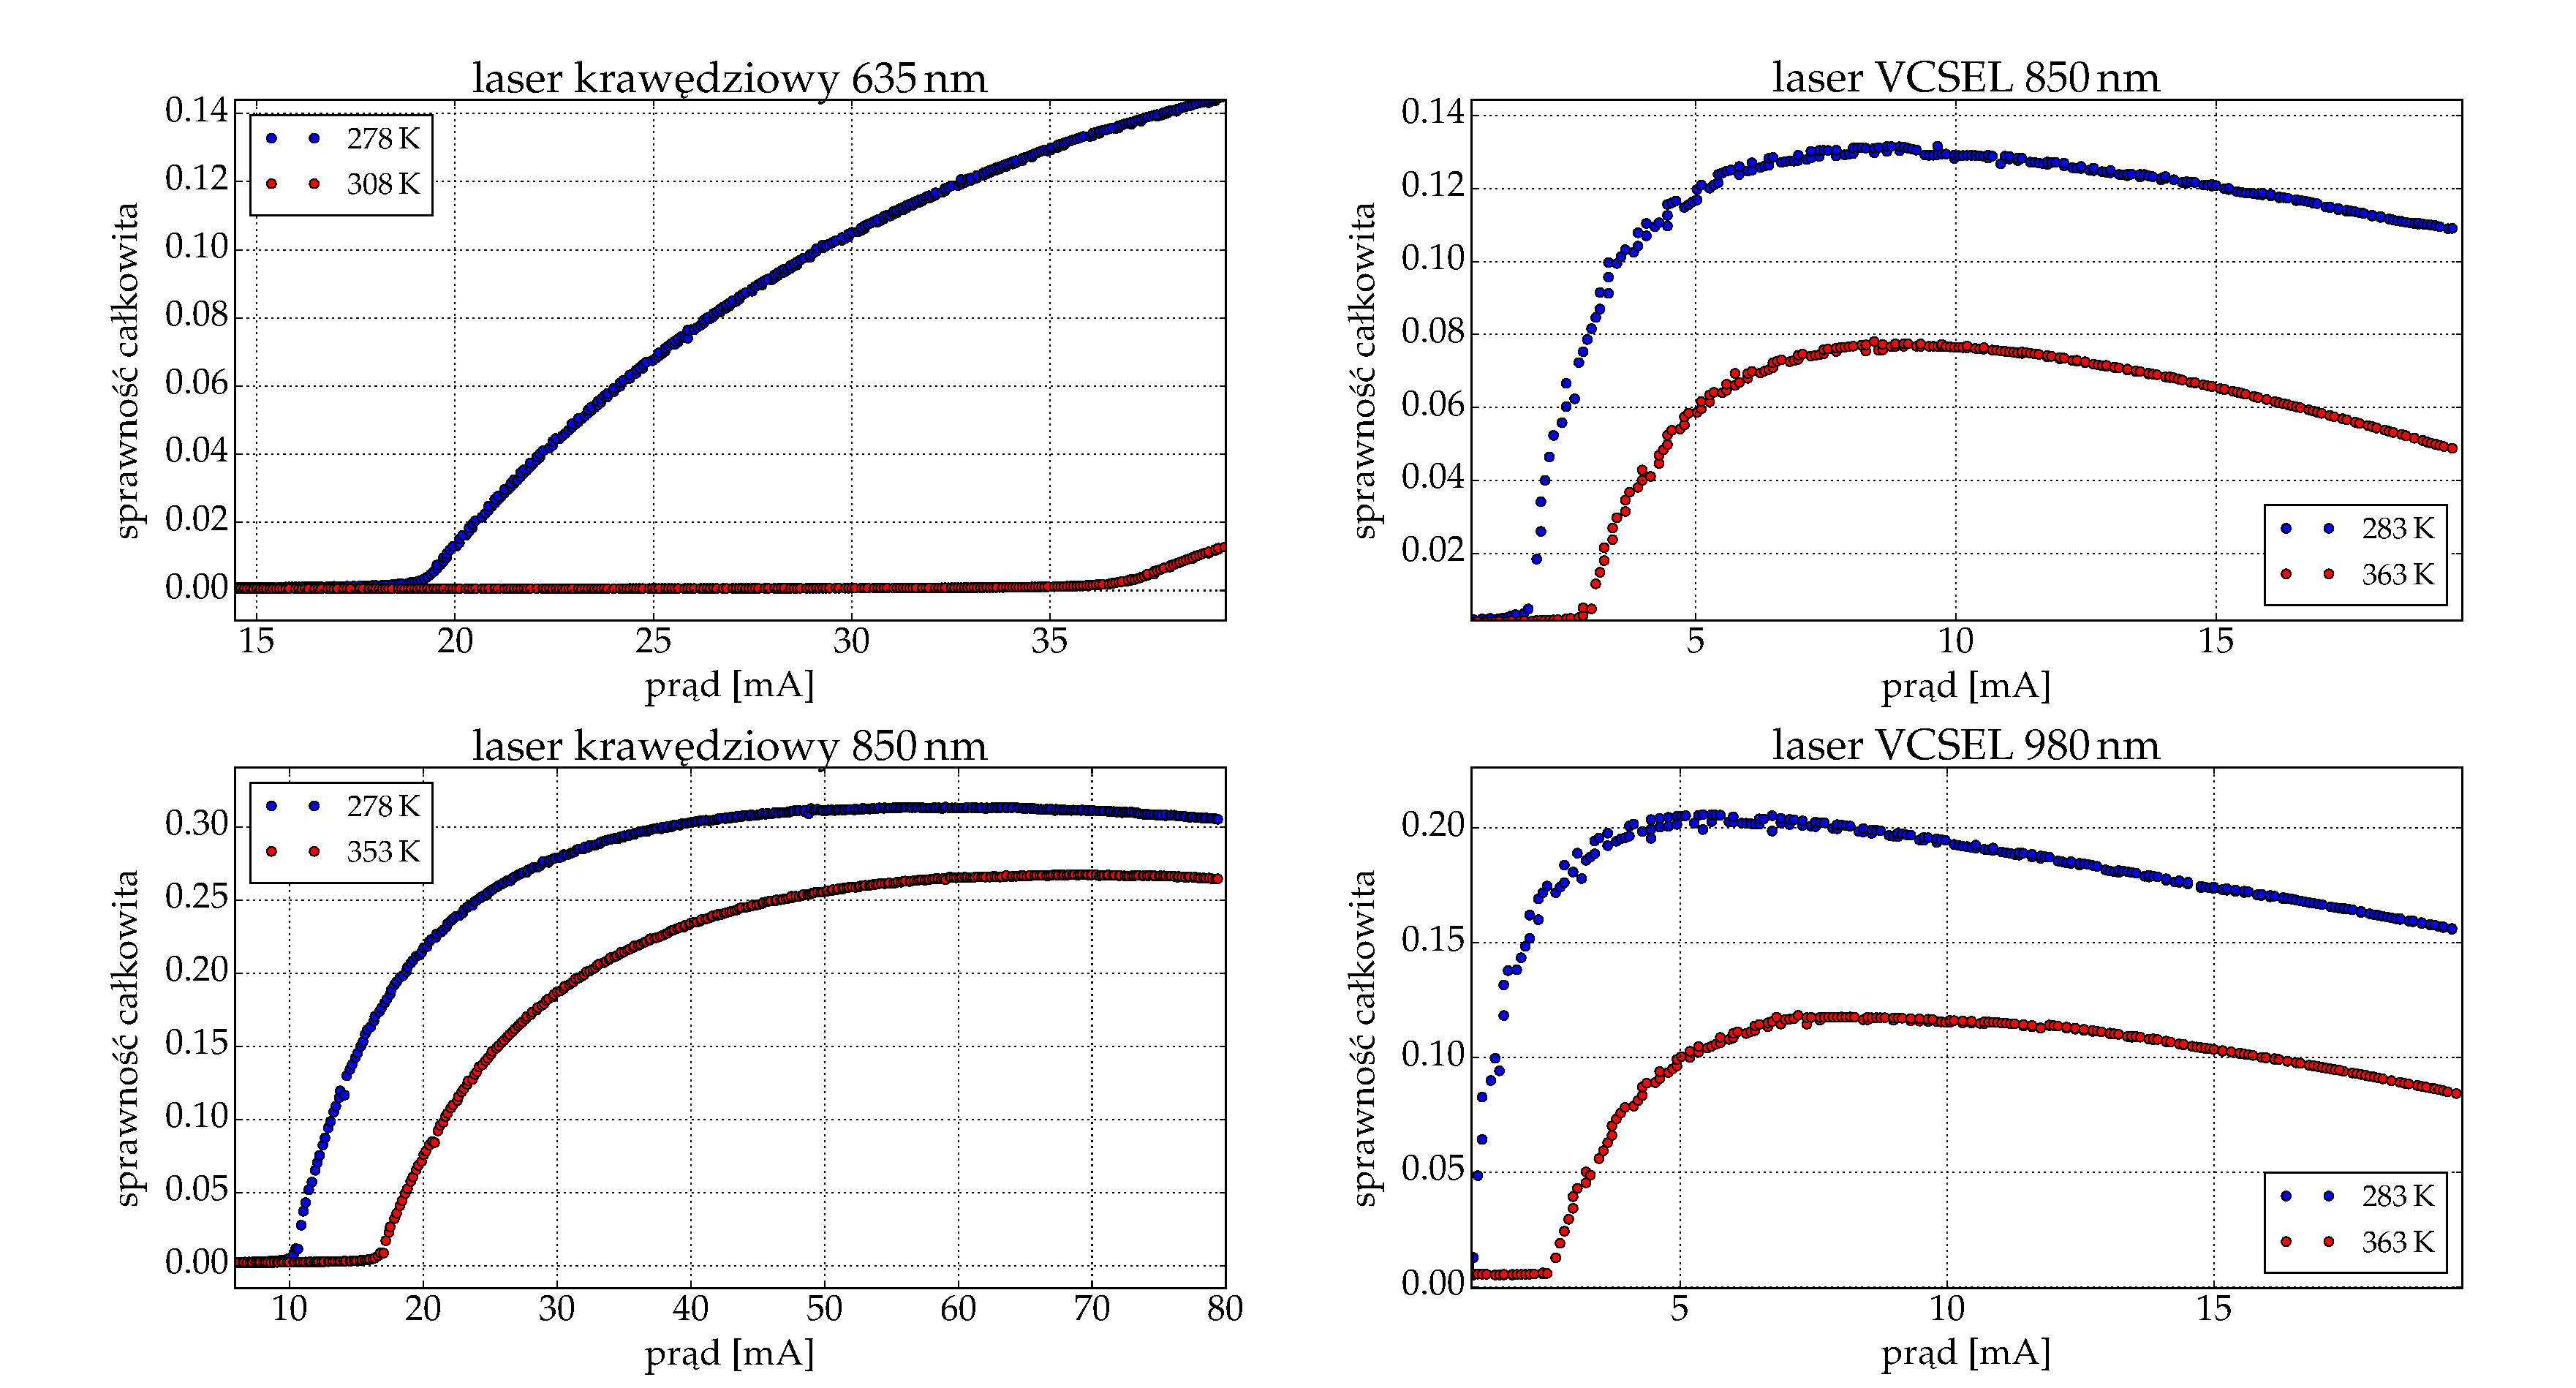
\includegraphics[scale=0.30]{plot_common/plot_wall_eff.eps}
  \caption{Wykres sprawności całkowitej w funkcji prądu.}
  \label{fig:plot_wall_eff}
\end{figure}
\newpage

\newpage
\chapter{Podsumowanie}
\section{Rezultat pracy}
W ramach pracy stworzyłem program do sterowania pomiarami charakterystyk elektryczno-optycznych laserów półprzewodnikowych.
Program stworzony jest
w dwóch wersjach: skryptowej oraz okienkowej. Program został napisany w języku Python w sposób obiektowy, co ułatwi
pracę nad nim w przyszłości. Praca moja wypełniła lukę, którą był brak programu do sterowania sprzętem firmy Thorlabs
na platformie Linux. W ramach pracy zbadałem 4 lasery półprzewodnikowe: dwa krawędziowe oraz dwa VCSEL. Wyznaczyłem dla nich
wartość prądu progowego oraz sprawności, które dobrze zgadzają się z wartościami z katalogu firmy Thorlabs. Otrzymane wyniki
przemawiają, za możliwością wykorzystania mojego programu do badania charakterystyk laserów.
\section{Co dalej?}
Możliwa jest dalszy rozwój programu m.in. o sterowanie zasilaniem impulsowym. Dołączenie oscyloskopu do układu pomiarowego pozwoli badać więcej cech
laserów półprzewodnikowych. Komunikacja z oscyloskopem będzie możliwa za pomocą klasy $\mathtt{IODevice.py}$.


\begin{thebibliography}{99}
\bibitem{python}
\emph{https://mycarta.wordpress.com/2016/09/16/python-and-the-discovery-of-gravitational-waves/}
dostęp 13.02.2017

\bibitem{matplotlib_book}  A.~Devert:
\emph{matplotlib Plotting Cookbook},
Packt Publising Ltd. 2014

\bibitem{SciPy_book} E.~Bressert:
\emph{Scipy and NymPy},
O'Reilly 2013

\bibitem{Ldc_book} Thorlabs Manual:
\emph{LDC4000 Series Operation Manual},
2016

\bibitem{Ldc_book_prog} Thorlabs Manual:
\emph{Series 4000 SCPI Programmer's Reference Manual},
2015

\bibitem{Pm100_book} Thorlabs Manual:
\emph{Operation Manual
Thorlabs Instrumentation Optical Power and Energy Meter PM100 USB},
2011

\bibitem{opto_book}  B.~Ziętek:
\emph{Optoelektronika},
Wydawnictwo Uniwersytetu Mikołaja Kopernika, Toruń, 2004

\bibitem{laser_book}  B.~Ziętek:
\emph{Lasery},
Wydawnictwo Uniwersytetu Mikołaja Kopernika, Toruń, 2009

\bibitem{publikcja_nakwaski} Włodzimierz Nakwaski, Robert P. Sarzała:
\emph{Lasery półprzewodnikowe}
 Przegląd Elektrotechniczny 2015 9

\bibitem{publikcja_magda} Magdalena MARCINIAK, Patrycja
ŚPIEWAK, Marta WIĘCKOWSKA, Robert Piotr SARZAŁA:
\emph{Mody poprzeczne w azotkowym laserze typu VCSEL}
 Przegląd Elektrotechniczny 2015 9

\bibitem{publikacja_1} B. Tell, K. F. Brown-Goebeler, R. E. Leibenguth, F. M.  Baez, Y. H. Leec:
\emph{Temperature dependence of GaAs-AIGaAs vertical cavity surface emitting lasers }
1991

\bibitem{praca_dok} Michał Baranowski:
\emph{Dynamika nośników w półprzewodnikowych
studniach kwantowych na podłożu z GaAs, emitujących w zakresie bliskiej podczerwieni.}
Praca doktorska, Politechnika Wrocławska
Instytut Fizyki, Wrocław 2013

\bibitem{spec_vcsel_850} Thorlabs:
MFG Spec,
\emph{VCSEL-980-MFGSpec}

\bibitem{spec_vcsel_980} Thorlabs:
MFG Spec,
\emph{VCSEL-980-MFGSpec}

\bibitem{spec_edge_850} Thorlabs
Spec Sheet
\emph{L850P010-SpecSheet}

\bibitem{spec_edge_635} Thorlabs
Spec Sheet
\emph{L635P003-SpecSheet}
\end{thebibliography}

\end{document}
\grid
